% = = = = = = = = = = = = = = = = = = = = = = = = = = = = = = = = = = = = = = = = = = = = =
% P  R  E  A  M  B  L  E
% = = = = = = = = = = = = = = = = = = = = = = = = = = = = = = = = = = = = = = = = = = = = =
\documentclass[11pt]{article}
\usepackage{amsbsy, amsmath, amssymb, authblk}

%\usepackage{array} 
%\usepackage{algorithm2e}

\usepackage{booktabs, bm}
\usepackage[small,labelfont=bf,up,singlelinecheck=false]{caption}
\usepackage{cancel}
\usepackage{comment}

%\usepackage{fancyhdr}
%\usepackage[default]{lato}
\usepackage[T1]{fontenc}
\usepackage[bottom]{footmisc}
\usepackage{geometry}
\usepackage{graphicx}
\usepackage{hyperref}
%\usepackage[utf8]{inputenc}
%	\inputencoding{latin1}
%	\inputencoding{utf8}
%\usepackage{lettrine}
%\usepackage[sc]{mathpazo}
\usepackage{lmodern} % Nice fonts?
%\usepackage{mathrsfs}
\usepackage{mathtools} 
%\usepackage{marvosym} % silly bullet-point symbols (misc symbols)
%\usepackage{microtype}
\usepackage{minitoc}         % left in case it is needed elsewhere
\setcounter{secttocdepth}{5} % idem
\usepackage{etoc} % for toc before each section.
%\usepackage{multicol}
\usepackage{needspace}
\usepackage{paralist}
%\usepackage{polynom} 			% typesetting polynomial long division
%\usepackage{setspace}
%	\onehalfspacing 
\usepackage{stmaryrd}  % \llbracket, \rrbracket
\usepackage{tocloft}
\usepackage{xparse} % DeclareDocumentCommand
\usepackage[compact]{titlesec} 		% compact shrinks whitespace around section headings.
\usepackage{ulem} 				% for strikeout \sout command.
%\usepackage{verbatim}

% Muh packagez :)
\usepackage{../Packages/MathCommands}
\usepackage{../Packages/BrandonColors}
\usepackage{../Packages/BrandonBoxes}
\usepackage{../Packages/NoteTaker}
%\usepackage{../Packages/MachineLearningUtils}

% NB: this has to be here for some reason
\usepackage{enumitem}  % using label=(\alph*)) in enumerate


%\usepackage{showframe} % Displays layout frame on all pages
\usepackage{marginnote}
\renewcommand*{\marginfont}{\scriptsize}
\usepackage{listings}

\usepackage{tikz}
\usetikzlibrary{arrows, automata, shapes, snakes, positioning}
\usetikzlibrary{bayesnet}

% hi?
\renewcommand\dotseq[2]
{#1^{(1)}, \ldots, #1^{(#2)}}
\renewcommand\rdotseq[2]
{#1^{(#2)}, \ldots, #1^{(1)}} % reversed


%\setlength{\parskip}{1pt}
%\setlength{\columnseprule}{0.1pt}
%\setlength{\columnsep}{0.6cm}
%\setlength\tabcolsep{0.1cm}
\renewcommand{\arraystretch}{1.2}

\DeclareDocumentEnvironment{definition}{O{-0.5em} o}{
	\IfNoValueTF{#2}{}{\textbf{#2}}
	\vspace*{#1}
	\begin{quote}
		\itshape\small}
	{\end{quote}}

% author, title, affiliation, date.
\DeclareDocumentCommand{\citepaper}{ m m m m }{
	\vspace{-1em}
	{\footnotesize #1, ``#2'' \textit{#3}, (#4).}
}


% Title
\title{\vspace{-10mm}\fontsize{24pt}{8pt}\selectfont\textbf{Fall 2016 Course Notes}\vspace*{-4mm}}
% Author
\author{Brandon McKinzie}
% Date
\date{}

\begin{document}
\dosecttoc
\tableofcontents

% ==================================================================================
% ==================================================================================
% ==================================================================================
% PGMS
% ==================================================================================
% ==================================================================================
% ==================================================================================
\mysection{Probabilistic Graphical Models}\label{Probabilistic Graphical Models}




\newcommand{\sep}{\text{sep}_{\mathcal{H}}}
\newcommand{\Y}{\matr{Y}}
\renewcommand{\Z}{\matr{Z}}



% ======================================================================================
\lecture{Probabilistic Graphical Models}{Foundations (Ch. 2)}{May 13, 2018}
% ======================================================================================

\vspace{-1em}
{\footnotesize (Brief summary of the book's notation, for ease of reference.)}

\p \blue{Graphs}. Authors denote directed graphs as $\mathcal G$ and undirected graphs as $\mathcal H$. 
\begin{compactitem}
	\item \green{Induced Subgraph}. Let $\mathcal K = (\mathcal X, \mathcal E)$ and $\matr{X} \subset \mathcal X$. Define the \textit{induced subgraph} $\mathcal{K}[\matr{X}]$ to be the graph $(\matr{X}, \mathcal{E}')$ where $\mathcal{E}'$ are all edges $X \rightleftharpoons Y$ such that $X, Y \in \matr{X}$.
	
	\item \green{Complete Subgraph}. A subgraph over $\matr{X}$ is \textit{complete} if every two nodes in $\matr{X}$ are connected by some edge. The set $\matr{X}$ is often called a \textit{clique}; we say that a clique $\matr{X}$ is \textit{maximal} if for any superset of nodes $\matr{Y} \supset \matr{X}$, $\matr{Y}$ is not a clique.
	
	\item \green{Upward Closure}. We say that a subset of nodes $\matr{X} \in \mathcal X$ is \textit{upwardly closed} in $\mathcal K$ if $\forall X \in \matr{X}$, we have that $\text{Boundary}_X \subset \matr X$\footnote{$\text{Boundary}_X \triangleq \text{Pa}_X \cup \text{Nb}_X$. For DAGs, this is simply $X$'s parents, and for undirected graphs $X$'s neighbors.}. We define the \textit{upward closure} of $\matr{X}$ to be the minimally upwardly closed subset $\matr{Y}$ that contains $\matr{X}$. We define the \textit{upwardly closed subgraph} of $\matr{X}$, denoted $\mathcal{K}^+[\matr{X}]$, to be the induced subgraph over $\matr{Y}$, $\mathcal{K}[\matr{Y}]$. 
\end{compactitem}

\myspace
\p \blue{Paths and Trails}. Definitions for longer-range connections in graphs. We use the notation $X_i \rightleftharpoons X_{j+1}$ to denote that $X_i$ and $X_j$ are connected via some edge, whether directed (in any direction) or undirected. 
\begin{compactitem}
	\item \green{Trail/Path}. We say that $X_1, \ldots, X_k$ form a \textit{trail} in the graph $\mathcal K = (\mathcal X, \mathcal E)$ if $\forall i = 1, \ldots, k - 1$, we have that $X_i \rightleftharpoons X_{j + 1}$. A \textit{path} makes an additional restriction: either $X_i \rightarrow X_{i + 1}$ or $X_i \text{---} X_{i + 1}$.
	
	\item \green{Connected Graph}. A graph is \textit{connected} if $\forall X_i, X_j$ there is a trail between $X_i$ and $X_j$. 
	
	\item \green{Cycle}. A \textit{cycle} in $\mathcal K$ is a directed path $X_1, \ldots X_k$ where $X_1 = X_k$. 
	
	\item \green{Loop}. A \textit{loop} in $\mathcal K$ is a trail where $X_1 = X_k$. A graph is \textit{singly connected} if it contains no loops. A node in a singly connected graph is called a \textit{leaf} if it has exactly one adjacent node. 
	
	\item \green{Polytree/Forest}. A singly connected graph is also called a \textit{polytree}. A singly connected undirected graph is called a \textit{forest}; if a forest is also connected, it is called a \textit{tree}.
	\begin{compactitem}
		\item A directed graph is a forest if each node has at most one parent. A directed forest is a tree if it is also connected.
	\end{compactitem} 
	
	\item \green{Chordal Graph}. Let $X_1 \text{---} X_2 \text{---} \cdots \text{---} X_k \text{---} X_1$ be a loop in the graph. A \textit{chord} in the loop is an edge connecting $X_i$ and $X_j$ for two nonconsecutive nodes $X_i$, $X_j$. An undirected graph $\mathcal H$ is said to be \textit{chordal} if any loop $X_1 \text{---} X_2 \text{---} \cdots \text{---} X_k \text{---} X_1$ for $k \ge 4$ has a chord. 
\end{compactitem}

\myspace
\p \blue{Probability}. Some notational reminders for this book. Let $\Omega$ denote a space of possible outcomes, and let $S$ denote a set of measurable \green{events} $\alpha$, each of which are a subset of $\Omega$.
\vspace{-0.5em}
\begin{quote}
	{\footnotesize\itshape 
		A probability distribution $P$ over $(\Omega, S)$ is a mapping from events in $S$ to real values that satisfy:
		\begin{compactitem}
			\item $P(\alpha) \ge 0$ for all $\alpha \in S$. 
			\item $P(\Omega) = 1$.
			\item If $\alpha, \beta \in S$ and $\alpha \cap \beta = \varnothing$, then $P(\alpha \cup \beta) = P(\alpha) + P(\beta)$.
		\end{compactitem}	
	}
\end{quote}
Some useful independence properties:
\begin{align}
	 \mtgreen{Symmetry}:\qquad			&(X \perp Y \mid Z) \implies (Y \perp X \mid Z) \\
	 \mtgreen{Decomposition}:\qquad	&(X \perp (Y, W) \mid Z) \implies (X \perp Y \mid Z)  \\
	 \mtgreen{Weak Union}:\qquad 		&(X \perp (Y, W) \mid Z) \implies (X \perp Y \mid Z, W) \\
	 \mtgreen{Contraction}:\qquad 	&(X \perp W \mid Z, Y) \& (X \perp Y \mid Z) \implies (X \perp Y, W \mid Z)
\end{align}
\begin{example}[My Proofs: Independence Properties]
I'll be using the definition that $(X \perp Y \mid Z) \Leftrightarrow P(X, Y \mid Z)=P(X \mid Z)P(Y \mid Z)$. Given this definition the proof for the symmetry property is trivial. In what follows, I'll assume the LHS of the given implication is true, and then show that the RHS must hold as well. \\

\textbf{Decomposition}:
$$P(X, Y \mid Z) = \sum_w P(X, Y, w \mid Z) = \sum_w P(X \mid Z) P(Y, w \mid Z)  = P(X \mid Z) P(Y \mid Z) \quad \mgreen{\checkmark}$$

\textbf{Weak Union}: 
\begin{align}
	P(X, Y \mid Z, W) &= \frac{ P(X, Y, W \mid Z) }{ P(W \mid Z) } \\
	&= \frac{ P(X \mid Z) P(Y, W \mid Z) }{ P(W \mid Z) } \\
	&= \frac{  P(X \mid Z) P(W \mid Z) P(Y \mid Z, W) }{ P(W \mid Z) } \\
	&= P(X \mid Z, W) P(Y \mid Z, W) \quad \mgreen{\checkmark}
\end{align}

\p \textbf{Contraction}: 
\begin{align}
	P(X, Y, W \mid Z) 
	&= P(Y \mid Z) P(X, W \mid Z, Y)	\\
	&= P(Y \mid Z) P(X \mid Z, Y) P(W \mid Z, Y) \\
	&= P(X \mid Z) \left[  P(Y \mid Z) P(W \mid Z, Y) \right] \\
	&= P(X \mid Z) P(Y, W \mid Z) \quad \mgreen{\checkmark}
\end{align}
\end{example}

\Needspace{10\baselineskip}
We now define what ``positive distribution'' means, and a useful property of such distributions.
\vspace{-0.5em}
\begin{quote}
{\footnotesize\itshape
	A distribution $P$ is said to be \green{positive} if for all events $\alpha \in S$, such that $\alpha \ne \varnothing$, we have that $P(\alpha) > 0$. 	
}
\end{quote}
For positive distributions, and for mutually disjoint sets $\X, \Y, \Z, \matr W$, the \green{intersection} property also holds:
\begin{align}
	\mtgreen{Intersection}:\qquad (\X \perp \Y \mid \Z, \matr W) \& (\X \perp \matr W \mid \Z, \Y) \implies (\X \perp \Y, \matr W \mid \Z)
\end{align}


\myspace
\subsub{Appendix}
\myspace

Figured this would be a good place to put some of the definitions in the Appendix, too. \\

\p \blue{Information Theory} (A.1). 
\begin{compactitem}
	\item \green{Entropy}. Let $P(X)$ be a distribution over a random variable $X$. The \textit{entropy} of $X$ is defined as\marginnote{We treat $0 \log \inv{0} = 0$}[2em]. 
	\begin{align}
		&H_P(X) = \E[P]{\lg \inv{P(X)}} = \sum_x P(X = x) \lg \inv{P(X = x)} \\
		&0 \le H_P(X) \le \lg|Val(X)|
	\end{align}
	$H_p(X)$ is a lower bound for the expected number of bits required to encode instances sampled from $P(X)$. Another interpretation is that the entropy is a measure of our uncertainty about the value of $X$. 
	
	\item \green{Conditional Entropy}. The \textit{conditional entropy} of $X$ given $Y$ is 
	\begin{align}
		H_P(X \mid Y) &= H_P(X, Y) - H_P(Y) = \E[P]{\lg \inv{P(X \mid Y)}} \\
		H_P(X \mid Y) &\le H_P(X)
	\end{align}
	which captures the additional cost (in bits) of encoding $X$ when we're already encoding $Y$. 
	
	\item \green{Mutual Information}. The \textit{mutual information} between $X$ and $Y$ is 
	\begin{align}
		I_P(X; Y) &= H_P(X) - H_P(X \mid Y) = \E[P]{\lg \frac{P(X\mid Y)}{ P(X) } }
	\end{align}
	which captures how many bits we save (on average) in the encoding of $X$ if we know the value $Y$. 
	
	\item \green{Distance Metric}. A \textit{distance metric} is any distance measure $d$ evaluating the distance between two distributions that satisfies all of the following properties:
	\begin{compactitem}
		\item \textbf{Positivity}: $d(P, Q) \ge 0$ and $d(P, Q) = 0$ if and only if $P = Q$. 
		\item \textbf{Symmetry}: $d(P, Q) = d(Q, P)$. 
		\item \textbf{Triangle inequality}: For any three distributions $P$, $Q$, $R$, we have that
		\begin{align}
			d(P, R) \le d(P, Q) + d(Q, R)
		\end{align}
	\end{compactitem}
	
	\item \green{Kullback-Liebler Divergence}. Let $P$ and $Q$ be two distributions over random variables $X_1, \ldots X_n$. The relative entropy, or KL-divergence, of $P$ and $Q$ is 
	\begin{align}
		D(P \| Q) = \E[P]{\lg \frac{ P(X_1, \ldots, X_n ) }{ Q(X_1, \ldots, X_n) }  }
	\end{align}
	Note that this only satisfies the positivity property, and is thus not a true distance metric. 
\end{compactitem}

\myspace 
\p \blue{Algorithms and Algorithmic Complexity} (A.3). 
\begin{compactitem}
	\item \green{Decision Problems}. A decision problem $\Pi$ is a task that accepts an input (instance) $\omega$ and decides whether it satisfies a certain condition or not. The \textbf{SAT} problem accepts a formula in propositional logic and decides whether there is an assignment to the variables in the formula such that it evaluates to true. \textbf{3-SAT} restricts this to accepting only formulas in conjunctive normal form (CNF), and further restricted s.t. each clause contains at most 3 literals. 
	
	\item \green{P}. A decision problem is in the class $\mathcal P$ if there exists a deterministic algorithm that takes an instance $\omega$ and determines whether $\omega \in \mathcal{L}_{\Pi}$ (the set of instances for which a correct algorithm must return true), in polynomial time in the size of the input $\omega$. 
	
	\item \green{NP}. A \textit{non-deterministic algorithm} takes the general form: (1) nondeterministically guess some assignment $\gamma$ to the variables of $\omega$, (2) deterministically verify whether $\gamma$ satisfies the condition of the problem.The algorithm will repeat these steps until it produces a $\gamma$ that satisfies the problem. A decision problem $\Pi$ is in the class $\mathcal{N}\mathcal{P}$ if there exists a nondeterministic algorithm that accepts $\omega$ if and only if $\omega \in \mathcal{L}_{\Pi}$, and if the verification stage can be executed in polynomial time in the length of $\omega$.
	
	\item \green{NP-hard}. $\Pi$ is $\NP$-hard if for every DP $\Pi' \in \NP$, there is a polynomial-time transformation of inputs such that an input for $\Pi'$ belongs to $\mathcal{L}_{\Pi'}$ if and only if the transformed instance belongs to $\mathcal{L}_{\Pi}$. Note that $\NP$-hard is a superset of $\NP$.\marginnote{The SAT problem is $\NP$-hard.}[-1em]
	
	\item \green{NP-complete}. A problem $\Pi$ is said to be $\NP$-complete if it is both $\NP$-hard and in $\NP$. 
\end{compactitem}

\myspace\Needspace{16\baselineskip}
\p \blue{Combinatorial Optimization and Search} (A.4). Below, I'll outline some common search algorithms. These are designed to address the following task:
\vspace{-0.8em}
\begin{quote}
	{\itshape\small Given initial candidate solution $\sigma_{cur}$, a score function \texttt{score}, and a set of \green{search operators} $\mathcal{O}$, search for the optimal solution $\sigma_{best}$ that maximizes the value of $score(\sigma_{best})$}
\end{quote}

\begin{algorithm}[Greedy local search (Algorithm A.5)]
	Repeat the following until $didUpdate$ evaluates to $false$ at the end of an iteration.
	\begin{compactenum}
		\item Initialize $\sigma_{best} := \sigma_{cur}$.
		
		\item Set $didUpdate := false$.
		
		\item For each operator $o \in \mathcal{O}$, do:
		\begin{compactenum}
			\item Let $\sigma_{o} := o(\sigma_{best})$. 
			
			\item If $\sigma_{o}$ is legal solution, and $score(\sigma_{o}) > score(\sigma_{best})$, reassign $\sigma_{best} := \sigma_{o}$, and set $didUpdate := true$. 
		\end{compactenum}
		
		\item If $didUpdate == true$, go back to step 2. Otherwise terminate and return $\sigma_{best}$. 
	\end{compactenum}
\end{algorithm}

\begin{algorithm}[Beam search (Algorithm A.7)]
	We are given a \green{beam width} $K$. Initialize our \textit{beam}, the set of at most $K$ solutions we are currently tracking, to $\{\sigma_{cur}\}$. Repeat the following until termination\footnote{Termination condition could be e.g. an upper bound on number of iterations or on the improvement achieved in the last iteration.}:
	\begin{compactenum}
		\item Initial the set of successor states $H := \varnothing$. 
		
		\item For each solution $\sigma \in Beam$, and each operator $o \in \mathcal{O}$, insert a candidate successor state $o(\sigma)$ into $H$. 
		
		\item Set $Beam := KBestScore(H)$\footnote{Notice that this implies an underlying assumption of beam search: all successor states $\sigma \in H$ have scores greater than any of the states in the current beam. We always assume improvement.}.
	\end{compactenum}
	Once termination is reached, return the best solution $\sigma_{best}$ in $Beam$. 
\end{algorithm}

\myspace 
\p \blue{Continuous Optimization} (A.5). 
\begin{compactitem}
	\item \textbf{Line Search}. Method for adaptively choosing the step size (learning rate) $\eta$ at each training step. Assuming we are doing gradient ascent. We'd usually set the parameters $\theta$ at step $t + 1$ to $\theta^{(t)} + \eta \nabla f(\theta^{(t)})$. Line search modifies this by instead defining the ``line'' $g(\eta)$ below, and searching for the optimal value of $\eta$ along that line.
	\begin{align}
		g(\eta) &= \overrightarrow{\theta}^{(t)} + \eta \nabla f(\theta^{(t)}) \\
		\eta^{(t)} &= \argmax_{\eta}[ g(\eta) ] \\
		\theta^{(t + 1)} &\leftarrow \theta^{(t)} + \eta^{(t)} \nabla f(\theta^{(t)})
	\end{align}
	At risk of stating the obvious, $g(\eta)$ is referred to as a ``line'' because it's a function of the form \texttt{mx + b}. 
	
\end{compactitem}

% -----------------------
\subsub{L-BFGS}
% -----------------------

Some notes from the textbook ``Numerical Optimization'' (chapters 8 and 9).

\myspace
\p \blue{The BFGS Method} (8.1). Begin the derivation by forming the following quadratic model of the objective function $f$ at the current iterate\footnote{Recall that an ``iterate'' is just some variable that gets iteratively computed/updated. Fancy people with fancy words.} $\theta_t$:\marginnote{For $m_t(p)$, $p$ denotes the deviation at step $t$ from the current parameters $\theta_t$.}
\begin{align}
	m_t(p) &= f_t + \nabla f_t^T p + \onehalf p^T B_t p
\end{align} 
where $B_t$ is an $n \times n$ symmetric p.d. matrix that will be revised/updated every iteration (it is \textit{not} the Hessian!). The minimizer $p_t$ of this function can be written explicitly\marginnote{$\pderiv{}{p}\onehalf p^T B_t p = B_t p $}[2em]
\begin{align}
	p_t &= -B_t^{-1} \nabla f_t
\end{align}
is used as the search direction, and the new iterate is
\begin{align}
	\theta_{t + 1} &\leftarrow \theta_t + \alpha_t p_t
\end{align}
where the step length $\alpha_t$ is chosen to satisfy the \purple{Wolfe conditions}\footnote{The Wolfe conditions are the following sufficient decrease and curvature conditions for line search:
\begin{align}
	f(\theta_t + \alpha_t p_t) &\le f(\theta_t) + c_1 \alpha_t \nabla f_t^T p_t \\
	\nabla f(\theta_t + \alpha_t p_t)^T p_t &\ge c_2 \nabla f_t^T p_t
\end{align}
for some constant $c_1 \in (0, 1)$ and $c_2 \in (c_1, 1)$. 
}. This is basically Newton's method with line search, except that we're using the \textit{approximate Hessian} $B_t$ instead of the true Hessian. It would be nice if we could somehow avoid recomputing $B_t$ at each step. One proposed method involves imposing conditions on $B_{t + 1}$ based on the previous step(s). Require that $\nabla m_{t + 1}$ equal $\nabla f$ at the latest two iterates $\theta_t$ and $\theta_{t + 1}$. Formally, the two conditions can be written as
\begin{align}
	\nabla m_{t + 1} (-\alpha_t p_t) = \nabla f_{t + 1} - \alpha_t B_{t + 1} p_t &= \nabla f_t \\
	\nabla m_{t + 1} (0) &= \nabla f_{t + 1}
\end{align}
We can rearrange the first condition to obtain the \green{secant equation}:
\begin{align}
	H_{t + 1} y_t &= s_t  \quad \text{where} \\
	H_{t + 1} &\triangleq B_{t + 1}^{-1} \\
	s_t &\triangleq \theta_{t + 1} - \theta_t \\
	y_t &\triangleq \nabla f_{t + 1} - \nabla f_t
\end{align}
which is true only if $s_t$ and $y_t$ satisfy the \green{curvature condition}, $s_t^T y_t > 0$. The curvature condition is guaranteed to hold if we impose the Wolfe conditions on the line search. As is, this still has infinitely many solutions for $H_{t + 1}$. To determine it uniquely, we impose the additional condition that $H_{t + 1}$ is the closest of all possible solutions to the current $H_t$:
\begin{align}
	\min_H || H - H_t ||_W \quad \text{s.t.} \quad H=H^T, ~ Hy_t=s_t
\end{align}
where $||\cdot||_W$ is the \textit{weighted Frobenius norm}\footnote{
	\begin{align}
		|| H ||_W &\triangleq || W^{1/2} H W^{1/2} ||_F \\
		|| C ||_F^2 &\triangleq \sum_{i,j} c_{ij}^2
	\end{align}
}, and $W$ can be any matrix satisfying $W s_t = y_t$. For concreteness, assume that $W = \widetilde{G}_t$, where
\begin{align}
	\widetilde{G}_t &= \int_0^1 \nabla^2 f(\theta_t + \tau \alpha_t p_t) \mathrm{d}\tau 
\end{align}
The unique solution to $H_{t + 1}$ is given by 
\graybox{
	\mtred{(BFGS)} \qquad H_{t + 1} &= (I - \rho_t s_t y_t^T) H_t (I - \rho_t y_t s_t^T) + \rho_t s_t s_t^T \tlab{8.16}
}
where $\rho_t = 1 / (y_t^Ts_t)$. The BFGS is summarized in algorithm 8.1 below. \\

\purple{Algorithm 8.1} (BFGS Method). Given starting point $\theta_0$, convergence tolerance $\epsilon > 0$, and inverse Hessian approximation $H_0$. Initialize $t = 0$. While $|| \nabla f_t || > \epsilon$ do:
\begin{compactenum}
	\item Compute search direction $p_t = -H_t \nabla f_t$. 
	
	\item Set $\theta_{t + 1} = \theta_t + \alpha_t p_t$, where $\alpha_t$ is computed via line search to satisfy the Wolfe conditions. 
	
	\item Define $s_t = \theta_{t + 1} - \theta_t$ and $y_t = \nabla f_{t + 1} - \nabla f_t$. 
	
	\item Compute $H_t$ by means of equation \ref{8.16}. 
	
	\item Increment $t \mathrel{+}=  1$ and go back to step 1. 
\end{compactenum}


\myspace\Needspace{20\baselineskip}
\p \blue{L-BFGS}. Modifies BFGS to store a modified version of $H_t$ implicitly, by storing some number $m$ of vector pairs $\{s_i, y_i\}$, corresponding to the $m$ most recent time steps. We use a recursive procedure to compute $H_t \nabla f_t$ given the set of vectors. \\

\purple{Algorithm 9.1} (L-BFGS two-loop recursion) Subroutine of L-BFGS for computing $ H_t \nabla f_t$. We're given the current value of $\nabla f_t$, and we initialize $q$ to this value. 
\begin{compactenum}
	\item For $i$ in the range $[t - 1, t - m]$, compute
	\begin{align}
		\alpha_i &\leftarrow \rho_i s_i^T q \\
		q &\leftarrow q - \alpha_i y_i
	\end{align}
	
	\item Set $r \rightarrow H_t^0 q$. 
	
	\item For $i$ in the range $[t - m, t - 1]$, compute
	\begin{align}
		\beta &\leftarrow \rho_i y_i^T r \\
		r &\leftarrow r + s_i(\alpha_i - \beta)
	\end{align}
	
	\item Return result $H_t \nabla f_t = r$. 
\end{compactenum}

\purple{Algorithm 9.2} (L-BFGS). Given starting point $\theta_0$, integer $m > 0$, and initial $t = 0$. Repeat the following until convergence.
\begin{compactenum}
	\item Choose $H_t^0$. A popular choice is $H_t^0 := \gamma_t I$, where 
	$$
	\gamma_t \triangleq \frac{ s_{t - 1}^T y_{t - 1}  }{ y_{t - 1}^T y_{t - 1}  }
	$$
	
	\item Compute $p_t \leftarrow - H_t \nabla f_t$ from Algorithm 9.1. 
	
	\item Compute $\theta_{t + 1} \leftarrow \theta_t + \alpha_t p_t$, where $\alpha_t$ is chosen to satisfy the Wolfe conditions. 
	
	\item if $t > m$, discard $\{s_{t - m}, y_{t - m}  \}$. Compute and save $s_t$ and $y_t$. 
	
	\item Increment $t \mathrel{+}=  1$ and go back to step 1. 
\end{compactenum}



% -----------------------
\subsub{Exercises}
% -----------------------

Going through all the problems with a star for review. \\

\begin{example}[Exercise 2.4]
	\textit{Let $\alpha \in S$ be an event s.t. $P(\alpha) > 0$. Show that $P(\cdot \mid \alpha)$ satisfies the properties of a valid probability distribution.} 
	\tcblower 
\begin{compactitem}
	\item Show $P(\beta \mid \alpha) \ge 0$ for all $\beta \in S$.  By definition,
	\begin{align}
		P(\beta \mid \alpha) &= \inv{P(\alpha)} P(\alpha \cap \beta) 
	\end{align}
	and since the full joint $P \ge 0$ and since $P(\alpha) > 0$, we have the desired result. 
	
	\item Show $P(\Omega_\alpha) = 1$. Again, using just the definitions,
	\begin{align}
		P(\Omega_{\alpha}) &= \sum_{\beta \in S} P(\beta \mid \alpha) \\
		&= \inv{P(\alpha)} \sum_{\beta \in S} P(\alpha \cap \beta) \\
		&= \inv{P(\alpha)} \left( \sum_{\beta \in \alpha} P(\beta) + \sum_{\gamma \notin \alpha} P(\varnothing)  \right) \\
		&= \inv{P(\alpha)} \left( P(\alpha) + 0 \right) \\
		&= 1
	\end{align}
	
	\item Show, for any $\beta, \gamma \in S$, where $\beta \cap \gamma = \varnothing$, that $P(\beta \cup \gamma \mid \alpha) = P(\beta \mid \alpha) + P(\gamma \mid \alpha)$. 
	\begin{align}
		P(\beta \cup \gamma \mid \alpha) 
		&= \inv{P(\alpha)} P( (\beta \cup \gamma) \cap \alpha   ) \\
		&= \inv{P(\alpha)} P( (\beta \cap \alpha) \cup (\gamma \cap \alpha) ) \\
		&= \inv{P(\alpha)} \left( P(\beta \cap \alpha) + P(\gamma \cap \alpha)  \right) \\
		&= P(\beta \mid \alpha) + P(\gamma \mid \alpha)
	\end{align}
\end{compactitem}
\end{example}

\begin{example}[Exercise 2.16: Jensen's Inequality]
	\textit{Let $f$ be a concave function and $P$ a distribution over a random variable $X$. Then 
		\begin{align}
			\E[P]{f(X)} \le f(\E[P]{X})
		\end{align}
	Use this inequality to prove the following 3 properties.}
	\tcblower 
	\begin{compactitem}
		\item $H_P(X) \le \log| Val(X) |$. Let $f(u) := \lg(u)$ be our concave function.
		\begin{align}
			H_P(X) \triangleq \E[P]{\lg \inv{P(X)}} &= \E[P]{f(u)} \\
			&\le f(\E[p]{u})  = f\left(\sum_x u(x) P(x)\right) = f(|Val(X)|) = \lg|Val(X)| \\
		\end{align}

		
		\item $H_P(X) \ge 0$. 
		\begin{align}
			-H_P(X) &= - \E[P]{\lg\inv{P(X)}} \\
					&= \E[P]{\lg P(X)} \le 0
		\end{align}
		since $0 \le P(X=x) \le 1$ $\forall x$ (any term in the expectation where $P(X=x) = 0$ is equal to $0$, by definition). 
		
		\item $D(P || Q) \ge 0$. Use the same idea as in the first proof, but let $u(x) = Q(x)/P(x)$. 
		\begin{align}
			D(P || Q) &\triangleq \E[P]{\lg \left( P(X) / Q(X) \right)} = - \E[p]{f(u)} \\
			- \E[p]{f(u)} &\ge f  \left( \sum_x u(x) P(x) \right) = f(1) = 0
		\end{align}
	\end{compactitem}
\end{example}





% ======================================================================================
\lecture{Probabilistic Graphical Models}{The Bayesian Network Representation (Ch. 3)}{May 06, 2018}
% ======================================================================================
\vspace{-1.7em}
{\scriptsize Koller and Friedman (2009). The Bayesian Network Representation.\\ \textit{Probabilistic Graphical Models: Principles and Techniques}.\\ }

\p \textbf{Goal}: \textit{represent a joint distribution $P$ over some set of variables $\mathcal{X} = \{X_1, \ldots, X_n\}$.} Consider the case where each $X_i$ is binary-valued. A \textit{single} joint distribution requires access to the probability for each of the $2^n$ possible assignments for $\mathcal{X}$. The set of all such possible joint distributions,
\begin{align}
	\{ (p_1, \ldots, p_{2^n}) \in \R^{2^n} : \sum_{i = 1}^{2^n} p_i = 1   \label{general-joint-space}  \}
\end{align}
is a $2^n - 1$ dimensional subspace of $\R^{2^n}$. Note that each $p_i$ represents the probability for a unique instantiation of $\mathcal{X}$. Furthermore, in the general case, knowing $p_i$ tells you nearly nothing about $p_{j \ne i}$ -- i.e. you require an instantiation of $2^{n} - 1$ independent parameters to specify a given joint distribution.\marginnote{Understanding the exponential blowup.}[-7em] 

But it would be foolish to parameterize any joint distribution in this way, since we can often take advantage of independencies. Consider the case where each $X_i$ gives the outcome (H or T) of coin $i$ being tossed. Then our distribution satisfies $(\matr X \perp \matr Y)$ for any disjoint subsets fo the variables $\matr X$ and $\matr Y$. Let $\theta_i$ denote the probability that coin $i$ lands heads. The key observation is that you only need each of the $n$ $\theta_i$ to specify a unique joint distribution over $\mathcal{X}$, reducing the $2^{n} - 1$ dimensional subspace to an $n$ dimensional manifold in $\R^{2^n}$\footnote{\red{TODO}: Formally define this manifold using the same notation as in \ref{general-joint-space}. Edit: Not sure how to actually write it out, but intuitively it's because each of the $2^n$ $p_i$ values, when going from the general case to the case of i.i.d, become \textit{functions} of the $n$ $\theta_i$ values. Whereas before they were independent free parameters.}.\marginnote{Taking advantage of independencies.}[-5em] 


\myspace
\p \blue{The Naive Bayes Model}. Say we want to determine the intelligence of an applicant based on their grade G in some course, and their score $S$ on the SAT. A naive bayes model can be illustrated as below. 



\begin{center}
	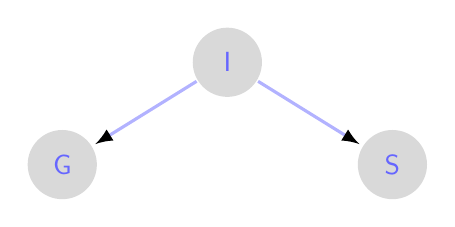
\begin{tikzpicture}[font=\sffamily,node distance=1.5cm,->,>=latex,auto,line width=0.4mm]
	
	\tikzset{node st/.style={state, draw=none,
			fill=gray!30!white,
			text=blue!60!white}}
	
	\node[node st] (I) {I};
	\node[below=2em of I] (dummy) {};
	\node[node st, left=of dummy] (G) {G};
	\node[node st, right=of dummy] (S) {S};  

	
	\draw[every loop,
	auto=right,
	draw=blue!30!white]
	(I) edge[->] node{} (G)
	(I) edge[->] node{} (S);

	\end{tikzpicture}
\end{center}
This encodes our general assumption that\footnote{We say that an event $\alpha$ is independent of event $\beta$ in $P$ with the notation $P \models (\alpha \perp \beta)$. (Def 2.2, pg 23 of book)} $P \models (S \perp G \mid I)$.

\myspace
\p In general, a naive bayes model assumes that instances fall into one of a number of mutually exclusive and exhaustive \textit{classes}, defined as the set of values that the top variable in the graph can take on\footnote{For the intelligence example, the classes are high intelligence and low intelligence.}. The model also includes some number of \textit{features} $X_1, \ldots X_k$, whose values are typically observed. The \green{naive Bayes assumption} is that the features are conditionally independent given the instance's class.

\myspace
\p \blue{Bayesian Networks}. A Bayesian network $\mathcal{B}$ is defined by a network structure together with its set of CPDs. \green{Causal reasoning} (or prediction) refers to computing the downstream effects of various factors (such as intelligence). \green{Evidential reasoning} (or explanation) is the reverse case, where we reason from effects to causes. Finally, \green{intercausal reasoning} (or explaining away) is when different causes of the same effect can interact. For our student example, we could be trying to determine $\Prob{I \mid G}$, the intelligence of an a student given his/her grade in a class. In addition to intelligence being a cause for the grade, we could have another causal variable $D$ for the difficulty of the class:

\begin{center}
	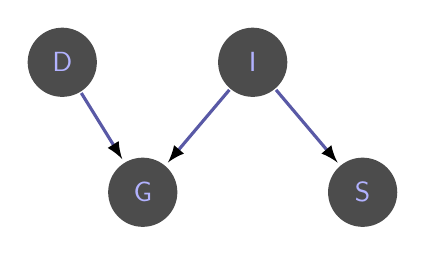
\begin{tikzpicture}[font=\sffamily,node distance=1.5cm,->,>=latex,auto,line width=0.4mm]
	
	\tikzset{node st/.style={state, draw=none,
			fill=gray!60!black,
			text=blue!30!white}}
	
	\node[node st] (I) {I};
	\node[node st, left=of I] (D) {D};
	
	\node[below=3em of I] (dummy) {};
	\node[node st, left=0.8cm of dummy] (G) {G};
	\node[node st, right=0.8cm of dummy] (S) {S};  
	
	\draw[every loop,
		auto=right,
		draw=blue!30!gray]	
	(I) edge[->] node{} (G)
	(I) edge[->] node{} (S)
	(D) edge[->] node{} (G);
	
	\end{tikzpicture}
\end{center}

An example of intercausal reasoning would be observing $D$, so that we now we want $\Prob{I \mid G, d}$; the diffulty of the course can help \textit{explain away} good/bad grades, thus changing our value for the probability of intelligence based on the grade alone. \\

A \green{Bayesian network structure} $\mathcal{G}$ is a DAG whose nodes represent RVs $X_1, \ldots X_n$. Let $Pa_{X_i}^{\mathcal{G}}$ denote the parents of $X_i$ in $\mathcal G$, and $\text{NonDesc}_{X_i}$ denotes the variables that are NOT descendants of $X_i$. Then $\mathcal G$ encodes the following set of \purple{\textit{local independencies}},
	\begin{align}
	\mathcal{I}_{\ell}(\mathcal G) \triangleq \{  \forall X_i : (X_i \perp \text{NonDesc}_{X_i} \mid Pa_{X_i}^{G})  \}
	\end{align}


\myspace
\p \blue{Graphs and Distributions}. Here we see that a distribution $P$ satisfies the local independencies associated with a graph $\mathcal G$ iff $P$ is representable as a set of CPDs associated with $\mathcal G$.  
\begin{compactitem}
	\item \textbf{Local independencies}. Let $P$ be a distribution over $\mathcal{X}$. We define $\mathcal I (P)$ to be the set of \green{independence assertions} of the form $(\matr X \perp \matr Y \mid \matr Z)$ that hold in $P$. The statement ``$P$ satisfies the local independencies associated with $\mathcal G$'' can thus be succinctly written:
	\begin{align}
		\mathcal{I}_{\ell}(\mathcal G) \subseteq \mathcal{I}(P)
	\end{align}
	and we'd say that $\mathcal G$ is an \green{I-map} (independency map) for $P$. 
	
	\item \textbf{I-maps}. More generally, let $\mathcal K$ be \textit{any} graph object associated with a set of independencies $\mathcal I(\mathcal K)$. We say that $\mathcal K$ is an \green{I-map} for a set of independencies $\mathcal I$ if $\mathcal I(\mathcal K) \subseteq \mathcal I$. Note that the complete graph (every two nodes connected) is an I-map for any distribution. 
	
	\item \textbf{Factorization}. Let $\mathcal G$ be a BN graph over $X_1, \ldots, X_n$. We say that a distribution $P$ over the same space \green{factorizes} according to $\mathcal G$ if $P$ can be expressed as 
	\begin{align}
		P(X_1, \ldots, X_n) &= \prod_{i = 1}^n P(X_i \mid Pa_{X_i}^{\mathcal G})
	\end{align}
	For BNs, the following equivalence holds: 
	$$
		\mathcal G \text{ is an I-map for } P \iff P \text{ factorizes according to } \mathcal G
	$$
	
\end{compactitem}

\myspace
\p \blue{D-separation}. We want to understand when we can \textit{guarantee} that an independence $(\matr X \perp \matr Y \mid \matr Z)$ holds in a distribution associated with a BN structure $\mathcal G$. Consider a 3-node network consisting of X, Y, and Z, where X and Y are not directly connected. There are four such cases, which I've drawn below.\marginnote{The fourth trail is called a \textit{v-structure}.}[2em]


\begin{center}
	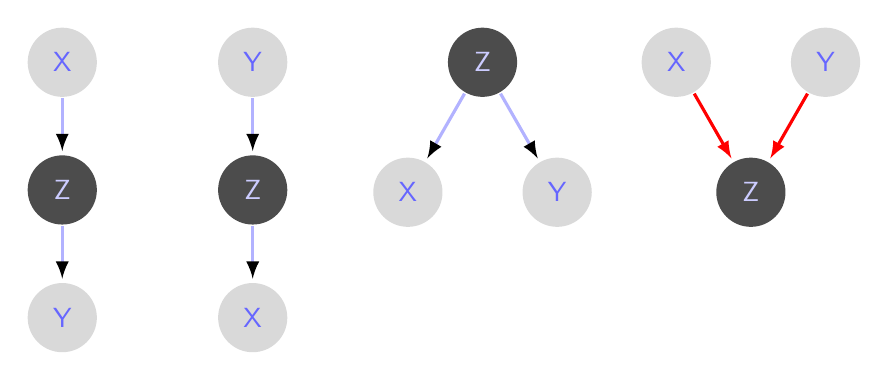
\begin{tikzpicture}[font=\sffamily,node distance=1.5cm,->,>=latex,auto,line width=0.4mm]
	
	\tikzset{node st/.style={state, draw=none,
			fill=gray!30!white,
			text=blue!60!white}}
	\tikzset{node obs/.style={state, draw=none,
			fill=gray!60!black,
			text=blue!20!white}}
	
	\node[node st] (X1) {X};
	\node[node obs, below=2em of X1] (Z1) {Z};
	\node[node st, below=2em of Z1] (Y1) {Y};
	
	
	\node[node st, right=of X1] (X2) {Y};
	\node[node obs, below=2em of X2] (Z2) {Z};
	\node[node st, below=2em of Z2] (Y2) {X};

	
	\node[node obs, right=2cm of X2] (Z3) {Z};
	\node[below=3em of Z3] (dummy1) {};
	\node[node st, left=1em of dummy1] (X3) {X};
	\node[node st, right=1em of dummy1] (Y3) {Y};

	
	\node[right=8em of Z3] (dummy2) {};
	\node[node st, left=1em of dummy2] (X4) {X};
	\node[node st, right=1em of dummy2] (Y4) {Y};
	\node[node obs, below=3em of dummy2] (Z4) {Z};

	
	\draw[every loop,
		auto=right,
		draw=blue!30!white]
	(X1) edge[->] node{} (Z1)
	(Z1) edge[->] node{} (Y1)
	(X2) edge[->] node{} (Z2)
	(Z2) edge[->] node{} (Y2)
	(Z3) edge[->] node{} (X3)
	(Z3) edge[->] node{} (Y3)
	(X4) edge[->, red] node{} (Z4)
	(Y4) edge[->, red] node{} (Z4);	
	\end{tikzpicture}
\end{center}
From left-to-right: indirect causal effect, indirect evidential effect, common cause, common effect. The first 3 satisfy $(X \perp Y \mid Z)$, but the 4th does not. Another way of saying this is that the first 3 trails are \green{active}\footnote{When influence can flow from X to Y via Z, we say that the trail $X \rightleftharpoons Y \rightleftharpoons Z$ is \textit{active}.} IFF $Z$ is not observed, while the 4th trail is active IFF $Z$ (or a descendent of $Z$) is observed. \\

\p \textbf{General case}:
\vspace{-0.5em}
\begin{quote}
	{\itshape Let $\mathcal G$ be a BN structure, and $X \rightleftharpoons \cdots \rightleftharpoons X_n$ a trail in $\mathcal G$. Let $\Z$ be a subset of observed variables. The trail is \green{active} given $\Z$ if 
		\begin{compactitem}
			\item Any v-structure $X_{i - 1} \rightarrow X_i \leftarrow X_{i + 1}$ has $X_i$ or one of its descendants in $\Z$.
			\item No other node along the trail is in $\Z$. 
		\end{compactitem}
	}
\end{quote}

\newcommand{\dsep}{\text{d-sep}_{\mathcal G}}
\p \textbf{D-separation}: (Directed separation)
\vspace{-0.5em}
\begin{quote}
	{\itshape Let $\X$, $\Y$, $\Z$ be three sets of nodes in $\mathcal G$. We say that $\X$ and $\Y$ are \green{d-separated} in $\mathcal G$, denoted $\dsep(\X; \Y \mid \Z)$, if there is no active trail between any node $X \in \X$ and $Y \in \Y$ given $\Z$. We use $\mathcal{I}(\mathcal G)$ to denote the set of independencies that correspond to d-separation,
		\begin{align}
			\mathcal{I}(\mathcal G) &= \{ \mred{\big(}  \X \perp \Y \mid \Z \mred{\big)}  : \dsep(\X ; \Y \mid \Z) \}
		\end{align}
		also called the set of \green{global Markov independencies}.
	}
\end{quote}

\myspace
\p \blue{Soundness and Completeness} of d-separation as a method for determining independence. 
\begin{compactitem}
	\item \textbf{Soundness} (Thm 3.3). If a distribution $P$ factorizes according to $\mathcal G$, then $\mathcal I(\mathcal G) \subseteq \mathcal I(P)$. 
	
	\item \textbf{Completeness}. For any distribution $P$ that factorizes over $\mathcal G$, we have that $P$ is \purple{faithful}\footnote{$P$ is faithful to $\mathcal G$ if, whenever $X \perp Y \mid \Z \in \mathcal{I}(P)$, then $\dsep(X; Y \mid \Z)$.} to $\mathcal G$: 
	\begin{align}
		X \perp Y \mid \Z \in \mathcal{I}(P) ~ \implies ~ \dsep(X; Y \mid \Z)
	\end{align}
\end{compactitem}
To see the detailed algorithm for finding nodes reachable from $X$ given $\Z$ via active trails, see Algorithm 3.1 on pg. 75 of the book.






% ======================================================================================
\lecture{Probabilistic Graphical Models}{Undirected Graphical Models (Ch. 4)}{November 03, 2017}
% ======================================================================================
\vspace{-1.7em}
{\scriptsize Koller and Friedman (2009). Undirected Graphical Models.\\ \textit{Probabilistic Graphical Models: Principles and Techniques}.\\ }


\p \blue{The Misconception Example}. Consider a scenario where we have four students who get together in pairs to work on homework for a class. Only the following pairs meet: (Alice, Bob), (Bob, Charles), (Charles, Debbie), (Debbie, Alice). The professor misspoke in class, giving rise to a possible misconception among the students. We have four binary random variables, $\{A, B, C, D\}$, representing whether the student has the misconception (1) or not (0) \footnote{A student might not have the misconception if e.g. they went home and figured out the problem via reading the textbook instead.}. Intuitively, we want to model a distribution that satisfies $(A \perp C \mid \{B, D\})$, and $(B \perp D \mid \{A, C\})$, but no other independencies\footnote{These independences cannot be naturally captured in a Bayesian (i.e. directed) network.}. Note that the interactions between variables seem symmetric here -- students influence each other (out of the ones they have a pair with). \\

\begin{center}
	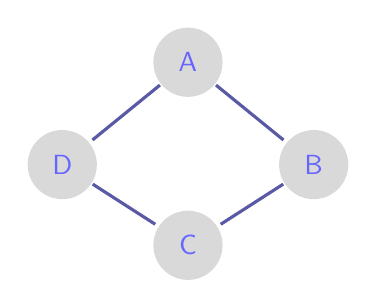
\begin{tikzpicture}[font=\sffamily,node distance=1.cm,->,>=latex,auto,line width=0.4mm]
	
	
	\tikzset{node st/.style={state, draw=none,
			fill=gray!30!white,
			text=blue!60!white}}
	\tikzset{node obs/.style={state, draw=none,
			fill=gray!60!black,
			text=blue!20!white}}
	
	\node[node st] (A) {A};
	\node[below=2em of A] (dummy) {};
	\node[node st, left=of dummy] (D) {D};
	\node[node st, right=of dummy] (B) {B};  
	\node[node st, below=4em of A] (C) {C};
	
	\draw[every loop,
		auto=right,
		draw=blue!30!gray]
	(A) edge[-] node{} (B)
	(A) edge[-] node{} (D)
	(B) edge[-] node{} (C)
	(D) edge[-] node{} (C);
	\end{tikzpicture}
\end{center}

The nodes in the graph of a \green{Markov network} represent the variables, and the edges correspond to a notion of direct probabilistic interaction between the neighboring variables -- an interaction that is not mediated by any other variable in the network. So, how should we parameterize our network? We want to capture the \green{affinities} between the related variables (e.g. Alice and Bob are more likely to agree than disagree).\marginnote{We restrict our attention to nonnegative factors.}[2em]
\begin{quote}
	{\itshape Let $\matr{D}$ be a set of random variables. We define a \green{factor} $\phi$ to be a function from $Val(\matr{D})$ to $\R$. A factor is nonnegative if all its entries are nonnegative. $\matr{D}$ is called the \green{scope} of the factor, denoted $Scope[\phi]$. 
	}
\end{quote}
The factors need not be normalized. Therefore, to interpret probabilities over factors, we must normalize it with what we'll call the \green{partition function}, $Z$:
\begin{align}
	\Prob{a, b, c, d} &= \inv{Z} \phi_1(a, b) \cdot \phi_2(b, c) \cdot \phi_3(c, d) \cdot \phi_4(d, a) \\
	Z &= \sum_{a, b, c, d} \phi_1(a, b) \cdot \phi_2(b, c) \cdot \phi_3(c, d) \cdot \phi_4(d, a)  
\end{align}

\myspace
\p \blue{Parameterization}. Associating the graph structure with a set of parameters. We parameterize undirected graphs by associating a set of factors with it. First, we introduce the definition of \green{factor product}:
\vspace{-0.5em}
\begin{quote}
	{\itshape Let $\matr{X}$, $\matr{Y}$, and $\matr Z$ be three disjoint sets of variables, and let $\phi_1(\matr X, \matr Y)$ and $\phi_2(\matr Y, \matr Z)$ be two factors. We define the \underline{factor product} $\phi_1 \times \phi_2$ to be a factor $\psi: Val(\matr X, \matr Y, \matr Z) \mapsto \R$ as follows:
		\begin{align}
			\psi(\matr X, \matr Y, \matr Z) = \phi_1(\matr X, \matr Y) \cdot \phi_2(\matr Y, \matr Z)
		\end{align}
	}
\end{quote}
We use this to define an undirected parameterization of a distribution:
\vspace{-1em}
\begin{quote}
	{\itshape A distribution $P_{\matr{\Phi}}$ is a \green{Gibbs distribution} parameterized by a set of factors $\matr{\Phi} = \{\phi_1(\matr[1]{D}, \ldots, \phi_K(\matr[K]{D}) )\}$ if it is defined as follows:
		\begin{align}
			P_{\matr{\Phi}} &= \inv{Z} \widetilde{P}_{\matr{\Phi}}(X_1, \ldots, X_n) \\
			 \widetilde{P}_{\matr{\Phi}}(X_1, \ldots, X_n) &= \phi_1(\matr[1]{D}) \times \phi_2(\matr[2]{D}) \times \cdots \times \phi_K(\matr[K]{D})
		\end{align}
	}
\end{quote}
where the authors (Koller and Friedman) have made a point to emphasize: \textbf{A factor is only one contribution to the overall joint distribution. The distribution as a whole has to take into consideration the contributions from all of the factors involved.} Now, we relate the parameterization of a Gibbs distribution to a graph structure.
\vspace{-0.5em}
\begin{quote}
	{\itshape A distribution $P_{\matr{\Phi}}$ with $\matr{\Phi} = \{\phi_1(\matr[1]{D}, \ldots, \phi_K(\matr[K]{D}) )\}$ \green{factorizes} over a Markov network $\mathcal{H}$ if each $\matr[k]{D} (k = 1, \ldots, K)$ is a complete subgraph\footnote{A subgraph is complete if every two nodes in the subgraph are connected by some edge. The set of nodes in such a subgraph is often called a \green{clique}. A clique $\matr{X}$ is maximal if for any superset of nodes $\matr{Y} \supset \matr{X}$, $\matr{Y}$ is \textit{not} a clique.} of $\mathcal{H}$.
	}
\end{quote}
The factors that parameterize a Markov network are often called \green{clique potentials}. Although it can be used without loss of generality, the parameterization using maximal clique potentials generally obscures structure that is present in the original set of factors. Below are some useful definitions that we will use often. \\

\p \textbf{Factor reduction}:
\vspace{-0.5em}
\begin{quote}
	{\itshape Let $\phi(\matr{Y})$ be a factor, and $\matr{U} = \vec{u}$ an assignment for $\matr U \subseteq \matr Y$. Define the \green{reduction} of the factor $\phi$ to the context $\matr U = \vec u$, denoted $\phi[\vec u]$, to be a factor over the scope $\matr{Y}' = \matr Y - \matr U$, such that
		\begin{align}
			\phi[\vec u](\vec{y}') = \phi(\vec{y}', \vec u)
		\end{align}
	For $\matr U \nsubseteq \matr Y$, define $\phi[\vec u]$ only for the assignments in $\vec u$ to the variables in $\matr{U}' = \matr U \cap \matr Y$. 
	}
\end{quote}

\p \textbf{Reduced Gibbs distribution}:
\vspace{-0.5em}
\begin{quote}
	{\itshape Let $P_{\matr{\Phi}}(\matr X)$ be a Gibbs distribution parameterized by $\matr{\Phi} = \{\phi_1, \ldots, \phi_K\}$ and let $\vec u$ be a context. The \green{reduced Gibbs distribution} $P_{\matr{\Phi}}[\vec u]$ is the Gibbs distribution defined by the set of factors $\matr{\Phi}[\vec u] = \{\phi_1[\vec u], \ldots, \phi_K[\vec u] \}$. More formally:
		\begin{align}
			P_{\matr{\Phi}}[\vec u] = P_{\matr{\Phi}}(\matr W \mid \vec u) \quad \text{where} \quad \matr W = \matr X - \matr U
		\end{align}
	}
\end{quote}

\p \textbf{Reduced Markov Network}:
\vspace{-1em}
\begin{quote}
	{\itshape Let $\mathcal H$ be a Markov network over $\matr{X}$ and $\matr{U} = \vec{u}$ a context. The \green{reduced Markov network} $\mathcal{H}[\vec{u}]$ is a Markov network over the nodes $\matr{W} = \matr{X} - \matr{U}$, where we have an edge $X \text{---} Y$ if there's an edge $X \text{---} Y$ in $\mathcal H$. 
	}
\end{quote}
Note that if a Gibbs distribution $P_{\Phi}(\matr{X})$ factorizes over $\mathcal H$, then $P_{\Phi}[\vec u]$ factorizes over $\mathcal{H}[\vec u]$. 

\myspace
\p \blue{Markov Network Independencies}. A formal presentation of the undirected graph as a representation of independence assertions.
\begin{compactitem}
	\item \green{Active Path}. Let $\mathcal H$ be a Markov network structure, and let $X_1 \text{---} \cdots \text{---} X_k$ be a path in $\mathcal H$. Let $\matr{Z} \subseteq \mathcal{X}$ be a set of \textit{observed variables}. The path is \textit{active} given $\matr{Z}$ if none of the $X_i$'s is in $\matr{Z}$. 
	
	\item \green{Separation}. A set of nodes $\matr{Z}$ \textit{separates} $\matr{X}$ and $\matr Y$ in $\mathcal H$, denoted $\text{sep}_{\mathcal H}(\matr X ; \matr Y \mid \matr Z)$, if there is no active path between any node $X \in \matr X$ and $Y \in \matr Y$ given $\matr  Z$. 
	
	\item \green{Global Independencies}. The \textit{global independencies} associated with $\mathcal H$ are defined as
	\begin{align}
		\mathcal{I}(\mathcal H) &= \{  (\matr X \perp \matr Y \mid \matr Z) : \text{sep}_{\mathcal H}(\matr X ; \matr Y \mid \matr Z)  \}
	\end{align}
	This is the \textit{separation criterion}. Note that the definition of separation is monotonic in $\matr{Z}$: if it holds for $\matr{Z}$, then it holds for any $\matr{Z}' \supset \matr{Z}$ as well\footnote{Which means that Markov networks are fundamentally incapable of representing nonmonotonic independence relations!}.
	
	\Needspace{15\baselineskip}
	\item \green{Soundness} of the separation criterion for detecting independence properties in distributions over $\mathcal{H}$. In other words, we want to prove that $$(P \text{ factorizes over }\mathcal{H}) \implies \big[\sep (\matr X ; \matr Y \mid \matr Z) \implies P \models (\matr X \perp \matr Y \mid \matr Z)\big]$$where the portion in brackets can equivalently be said as ``$\mathcal{H}$ is an I-map for $P$''. \\
	\begin{example}[Proof]
	\begin{compactitem}
		\item Consider the case where $\X \cup \Y \cup \Z = \mathcal{X}$. 
		
		\item Then, any clique in $\mathcal{X}$ is fully contained in either $\X \cup \Z$ or $\Y \cup \Z$. In other words,
		\begin{align}
			P(\X, \Y, \Z) &= \inv{Z} f(\X, \Z) g(\Y, \Z) \\
			\text{which implies}\quad
			P(\X, \Y \mid \Z) &= \dfrac{
				f(\X, \Z) g(\Y, \Z)
				}{
				\sum_{x, y} f(x, \Z) g(y, \Z)
				}
		\end{align}
		
		\item We can prove that $P \models (\X \perp \Y \mid \Z)$ by showing that $P(\X, \Y \mid \Z) = P(\X \mid \Z) P(\Y \mid \Z)$. 
		\begin{align}
			P(\X, \Y \mid \Z) &= \frac{f(\X, \Z) g(\Y, \Z)}{P(\Z)} \\
			&=  \frac{f(\X, \Z) g(\Y, \Z)}{P(\Z)} \frac{P(\Z)}{P(\Z)} \\
			&=  \frac{f(\X, \Z) g(\Y, \Z)}{P(\Z)} \frac{ \sum_x f(x, \Z) \sum_y g(y, \Z) }{ P(\Z) } \\
			&=  \frac{f(\X, \Z)  \sum_y g(y, \Z) }{P(\Z)} \frac{ g(\Y, \Z) \sum_x f(x, \Z)}{ P(\Z) } \\
			&= P(\X \mid \Z) P(\Y \mid \Z)
		\end{align} 
		
		\item For the general case where $\X \cup \Y \cup \Z = \mathcal{X}$, let $\matr{U} = \mathcal{X} - (\X \cup \Y \cup \Z )$. Since we know that $\sep (\matr X ; \matr Y \mid \matr Z)$, we can partition $\matr U$ into two disjoint sets $\matr[1]{U}$ and $\matr[2]{U}$ such that $\sep (\matr X \cup \matr[1]{U} ; \matr Y \cup \matr[2]{U}\mid \matr Z)$. Combining the previous result with the decomposition property\footnote{The decomposition property:$$(\X \perp (\Y, \matr{W}) \mid \Z) \implies (\X \perp \Y \mid \Z)$$} give us the desired result that $P \models (\X \perp \Y \mid \Z)$.
	\end{compactitem}
	\end{example}
\end{compactitem}

\myspace
\p \textbf{Pairwise Independencies}:
\vspace{-0.5em}
\begin{quote}
	{\itshape 
		Let $\mathcal H$ be a Markov network. We define the \green{pairwise independencies} assoc. with $\mathcal{H}$:
		\begin{align}
			\mathcal{I}_{p}(\mathcal H) &= \{ \mred{\big(} X \perp Y \mid \mathcal X  - \{X,Y\} \mred{\big)} ~ : ~ X\text{---}Y \notin \mathcal H  \}
		\end{align}
		which just says ``X is indep. of Y given everything else if there's no edge between X and Y.''
	}
\end{quote}

\newcommand\MB{\mathrm{MB}_{\mathcal H}}

\myspace
\p \textbf{Local Independencies}:
\vspace{-0.5em}
\begin{quote}
	{\itshape 
		For a given graph $\mathcal H$, define the \green{Markov blanket} of $X$ in $\mathcal H$, denoted $\MB(X)$, to be the neighbors of $X$ in $\mathcal{H}$. We define the \green{local independencies} associated with $\mathcal H$:
		\begin{align}
			\mathcal{I}_{\ell}(\mathcal H) &= \{ \mred{\big(}X \perp \mathcal X - \{X\}  - \MB(X) \mid \MB(X)  \mred{\big)}  ~ : ~ X \in \mathcal X   \}
		\end{align}
	}
	which just says ``X is indep. of the rest of the nodes in the graph given its immediate neighbors.''
\end{quote}

\myspace
\p \blue{Log-Linear Models}. Certain patterns involving particular values of variables for a given factor can often be more easily seen by converting factors into log-space. More precisely, we can rewrite a factor $\phi(\matr D)$ as
\begin{align}
	\phi(\matr D) &= e^{- \epsilon(\matr D)} \\
	\epsilon(\matr D) &\triangleq -\ln \phi(\matr D) \\
	\Prob{X_1, \ldots, X_n} &\propto e^{- \sum \epsilon_i(\matr[i]{D}   )}
\end{align} 
where $\epsilon(\matr D)$ is often called an \green{energy function}. Note how $\epsilon$ can take on any value along the real line (i.e. removes our nonnegativity constraint)\footnote{We seem to be implicitly assuming that the original factors are all \textit{positive} (not just non-negative).}. Also note that as the $\epsilon$ summation approaches 0, the probability approaches one. 

\myspace\Needspace{10\baselineskip}
This motivates introducing the notion of a \green{feature}, which is just a factor without the nonnegativity requirement. A popular type of feature is the \green{indicator feature} that takes on value 1 for some values $\vec y \in Val(\matr D)$ and 0 otherwise. We can now provide a more general definition for our notion of log-linear models:
\vspace{-0.5em}
\begin{quote}
	{\itshape
	A distribution $P$ is a \green{log-linear model} over a Markov network $\mathcal H$ if it is associated with:
	\begin{compactitem}
		\item A set of features $\mathcal F = \{ f_1(\matr[1]{D}), \ldots, f_k(\matr[k]{D})  \}$ where each $\matr[i]{D}$ is a complete subgraph (i.e. a clique)in $\mathcal H$. 
		\item A set of weights $w_1, \ldots, w_k$. 
	\end{compactitem} 
	such that
	\begin{align}
		\Prob{X_1, \ldots, X_n} &= \inv{Z} \exp \left[ - \sum_{i =1}^{k} w_i f_i(\matr[i]{D})  \right]
	\end{align}
	}
\end{quote}
The log-linear model provides a much more compact representation for many distributions, especially in situations where variables have large domains (such as text).\\
\begin{example}[Box 4.C -- Concept: Ising Models and Boltzmann Machines]
	The \green{Ising model}: Each atom is modeled as a binary RV $X_i \in \{+1, -1\}$ denoting its spin. Each pair of neighboring atoms is associated with energy function $\epsilon_{i,j}(x_i, x_j) = w_{i,j} x_i x_j$. We also have individual energy functions $u_i x_i$ for each atom. This defines our distribution:
	\begin{align}
		P(\xi) = \inv{Z} \exp \bigg( - \sum_{i < j} w_{i,j}x_i x_j - \sum_i u_i x_i   \bigg)
	\end{align}
	
	The \green{Boltzmann distribution}: Now the variables are $X_i \in \{0, 1\}$. The distribution of each $X_i$ given its neighbors is 
	\begin{align}
		P(x_i^1 \mid Nb(X_i)) &= \text{sigmoid}(z) \\
		z &= -(\sum_j w_{i,j} x_j  )-u_i
	\end{align}
\end{example}

\begin{example}[Box 4.D -- Concept: Metric MRFs]
	Consider the pairwise graph $X_1,\ldots, X_n$ in the context of sequence labeling. We want to assign each $X_i$ a label. We also want adjacent nodes to prefer being similar to each other. We usually use the MAP objective, so our goal will be to minimize the total energy over the parameters (which are given by the individual energy functions $\epsilon_i$).
	\begin{align}
		E(x_1, \ldots, x_n) &= \sum_i \epsilon_i (x_i) + \sum_{(i,j) \in \mathcal{E}} \epsilon_{i,j}(x_i, x_j)
	\end{align}
	The simplest place to start for preferring neighboring labels to take on similar values is to define $\epsilon_{i,j}$ to have low energy when $x_i = x_j$ and some positive $\lambda_{i,j}$ otherwise. We want to have finer granularity for our similarities between labels. To do this, we introduce the definition of a \green{metric}: a function $\mu : \mathcal V \times \mathcal V \mapsto [0, \infty)$ that satisfies
	\begin{align}
		\green{\text{[reflexivity]}}&  \qquad \mu(v_k, v_l) = 0 \quad \text{IFF} \quad k = l \\
		\green{\text{[symmetry]}}& \qquad \mu(v_k, v_l) = \mu(v_l, v_k) \\
		\green{\text{[triangle inequality]}}& \qquad \mu(v_k, v_l) + \mu(v_l, v_m) \ge \mu(v_k, v_m)
	\end{align}
	and we can now let $\epsilon_{i,j}(v_k, v_l) := \mu(v_k, v_l)$. 
\end{example}

\myspace
\p \blue{Canonical Parameterization} (4.4.2.1). Markov networks are generally overparameterized\footnote{Meaning: for any $P_{\Phi}$, there are often infinitely many ways to choose its set of parameter values for a given $\mathcal H$.}. The \green{canonical parameterization}, \underline{which requires that $P$ be positive}, avoids this. First, some notation and requirements:
\begin{compactitem}
	\item P must be positive. 
	\item Let $\xi^* = (x_1^*, \ldots, x_n^*)$ denote some fixed assignment to the network variables $\mathcal X$. 
	\item Define $\vec[\Z]{x} \triangleq \vec{x}\langle \Z \rangle$ as the assignment of variables in some subset $\Z$.\footnote{And $\vec x$ is some assignment to some subset of $\mathcal X$ that also contains $\Z$.}
	\item Define $\xi^*_{-\Z} \triangleq \xi^*\langle \mathcal X - \Z \rangle$ be our fixed assignment for the variables outside $\matr Z$. 
	\item Let $\ell(\xi)$ denote $\ln P(\xi)$.  
\end{compactitem}

\Needspace{10\baselineskip}
The \green{canonical energy function} for a clique $\matr D$ is defined below, as well as the associated total $P(\xi)$ over a full network assignment:\marginnote{The sum is over all subsets of $\matr D$, including $\matr D$ itself and $\varnothing$.}[1em]
\graybox{
	\epsilon^*_{\matr D}(\vec d) &= \sum_{\Z \subseteq \matr D} \ell(\vec[\Z]{d}, \xi^*_{-\Z}) \cdot (-1)^{|\matr D - \Z|} \\
	P(\xi) &= \exp\bigg[ \sum_i \epsilon^*_{\matr[i]{D}}(  \xi\langle \matr[i]{D} \rangle )     \bigg] \label{thm-4.7}
}


\myspace
\p \blue{Conditional Random Fields}. So far, we've only described Markov network representation as encoding a joint distribution over $\mathcal X$. The same undirected graph representation and parameterization can also be used to encode a \textit{conditional distribution} $\Prob{\matr Y \mid \matr X}$, where $\matr Y$ is a set of \textit{target variables} and $\matr X$ is a (disjoint) set of \textit{observed variables}.\marginnote{Note how there are no connection between any of the $X$s}[4em]
\begin{center}
	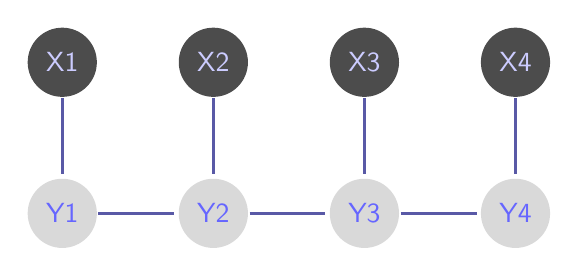
\begin{tikzpicture}[font=\sffamily,node distance=1.cm,->,>=latex,auto,line width=0.4mm]
		
		\tikzset{node st/.style={state, draw=none,
				fill=gray!30!white,
				text=blue!60!white}}
		\tikzset{node obs/.style={state, draw=none,
				fill=gray!60!black,
				text=blue!20!white}}
	
	\node[node obs] (X1) {X1};
	\node[node obs, right=of X1] (X2) {X2};
	\node[node obs, right=of X2] (X3) {X3};
	\node[node obs, right=of X3] (X4) {X4};

	\node[node st, below=of X1] (Y1) {Y1};
	\node[node st, right=of Y1] (Y2) {Y2};
	\node[node st, right=of Y2] (Y3) {Y3};
	\node[node st, right=of Y3] (Y4) {Y4};
	
	\draw[every loop,
		auto=right,
		draw=blue!30!gray]
	(X1) edge[-]				node{} (Y1)
	(X2) edge[-]				node{} (Y2)
	(X3) edge[-]				node{} (Y3)
	(X4) edge[-]				node{} (Y4)
	(Y1) edge[-] 				node{} (Y2)
	(Y2) edge[-] 				node{} (Y3)
	(Y3) edge[-] 				node{} (Y4);
	\end{tikzpicture}
\end{center}

\p Formally, a CRF is an undirected graph $\mathcal H$ whose nodes correspond to $\matr Y \cup \matr X$. Since we want to avoid representing\footnote{Also note how we never have to deal with a summation over all possible $\X$, due to restricting ourselves to $Z(\X)$.} a probabilistic model over $\matr X$, we disallow potentials that involve only variables in $\matr X$; our set of factors is $\phi_1(\matr[1]{D}), \ldots, \phi_m(\matr[m]{D})$, such that each $\matr[i]{D} \nsubseteq \matr{X}$. The network encodes a conditional distribution as follows:
\graybox{
	P(\Y \mid \X) &= \inv{Z(\X)} \widetilde{P}(\Y, \X)	\\
	 \widetilde{P}(\Y, \X) &= \prod_{i = 1}^{m} \phi_i(\matr[i]{D}) \\
	 Z(\matr X) &= \sum_{\matr Y}  \widetilde{P}(\matr Y, \X)
}
where now the partition function is a function of the assignment $\vec x$ to $\matr X$. 

\myspace
\p \blue{Rapid Summary}. 
\begin{compactitem}
	\item \textbf{Gibbs distribution}: any probability distribution that can be written as a product of factors divided by some partition function $Z$. 
	\item \textbf{Factorizes}: A Gibbs distribution factorizes over $\mathcal H$ if each factor [in its product of factors] is a clique. 
\end{compactitem}

\myspace
\subsub{Exercises}
\myspace

%\tikzstyle{gnode}=[state, fill=gray!60!black, text=blue!30!white, draw=none]
%\tikzstyle{myedge}=[-, orange]

\begin{example}[Exercise 4.1]
	\textit{Let $\mathcal{H}$ be the graph of binary variables below. Show that P does not factorize over $\mathcal{H}$ (Hint: proof by contradiction).}
	\begin{center}
		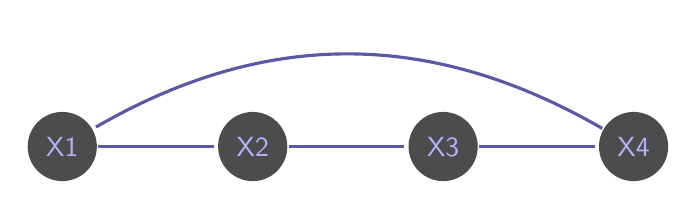
\begin{tikzpicture}[font=\sffamily,node distance=1.5cm,->,>=latex,auto,line width=0.4mm]
		
		\tikzset{node st/.style={state, draw=none,
								fill=gray!60!black,
								text=blue!30!white}}
		
		\node[node st] (X1) {X1};
		\node[node st, right=of X1] (X2) {X2};
		\node[node st, right=of X2] (X3) {X3};
		\node[node st, right=of X3] (X4) {X4};
		
		\draw[every loop,
			  auto=right,
			  draw=blue!30!gray]
		(X1) edge[-] 				node{} (X2)
		(X2) edge[-] 				node{} (X3)
		(X3) edge[-] 				node{} (X4)		
		(X4) edge[-, bend right] 	node{} (X1);				
		\end{tikzpicture}
	\end{center}
	\begin{compactitem}
		\item Example 4.4 recap: P satisfies the global independencies w.r.t $\mathcal{H}$. They showed this by manually checking the two global indeps of $\mathcal{H}$, $(X_1 \perp X_3 \mid X_2, X_4)$ and $(X_2 \perp X_4 \mid X_1, X_3)$, against the tabulated list of possible assignments for $P$ (given in example). Nothing fancy. 
		\item P factorizes over $\mathcal{H}$ if it can be written as a product of clique potentials.
		\item My proof:
		\begin{compactenum}
			\item Assume that $P$ \textit{does} factorize over $\mathcal{H}$.
			\item Then $P$ can be written as
			\begin{align}
				P(X_1, X_2, X_3, X_4) &= \inv{Z} \phi_1(X_1, X_2) \phi_2(X_2, X_3) \phi_3(X_3, X_4) \phi_4(X_4, X_1)
			\end{align}
			
			Let the above assertion be denoted as $C$, and the statement that $P$ factorizes according to $\mathcal{H}$ be denoted simply as $P_{\mathcal H}$. Since $P_{\mathcal H} \iff C$, if we can prove that $C$ does not hold, then we've found our contradiction, meaning $P_{\mathcal{H}}$ also must not hold.
			
			\item I know that the proof must take advantage of the fact that we know $P$ is zero for certain assignments to $\mathcal{X}$. For example $P(0100) = 0$. Furthermore, by looking at the assignments where $P$ is \textit{not} zero, I can see that all possible combinations of $(X_1, X_2)$ are present, which means $\phi_1$ never evaluates to zero.
			
			\item From the example, we know that $P(1100) = 1/8 \ne 0$. However, since
			\begin{align}
				0 = \frac{P(0100)}{P(1100)} &= \frac{\phi_1(0, 1)\phi_4(0, 0)}{\phi_1(1, 1)\phi_4(0, 1)} \\
			   &= \frac{\phi_4(0, 0)}{\phi_4(0, 1)} \qquad \mred{(\phi_1 > 0)} \label{idkhi}
			\end{align}
			and we also know that both the numerator and denominator of eq. \ref{idkhi} are positive, and thus we have a contradiction. 
		\end{compactenum}
	\end{compactitem}
\end{example}

\begin{example}[Exercise 4.4]
\textit{Prove theorem 4.7 for the case where $\mathcal H$ consists of a single clique.} Theorem 4.7 is equation \ref{thm-4.7} in my notes. For a single clique $\matr D$, the question reduces to: Show that, for any assignment $\vec d$ to $\matr D$:
\begin{align}
	P(\vec d)
	&=  \frac{\exp\bigg( -\epsilon(\vec d)   \bigg)   }{   \sum_{\vec{d}'} \exp\bigg( -\epsilon(\vec{d}')   \bigg)   }    \\
	&= \exp\bigg( \epsilon^*_{\matr D} ( \vec d )  \bigg)
\end{align}

Consider the case where $|\matr D|= 1$, i.e. $\vec d = d$ is a single variable. Then
\begin{align}
	\epsilon^*_{\matr D}(\vec d) 
	&= (-1)^{|\matr D|} \ell(\xi^*_{\matr D}) + (-1)^{|\matr D - \matr D|}\ell(\vec d) \\
	&= -\ell(\xi^*_{\matr D}) + \ell(\vec d) \\
	&= -\ln P(d^*) + \ln P(d)
\end{align}
and therefore
\begin{align}
	 \exp\bigg( \epsilon^*_{\matr D} ( \vec d )  \bigg)
	 &= P(d) / P(d^*)
\end{align}
which is clearly incorrect (???) \red{TODO}: figure out what's going on here. Either the book has a type in its for theorem 4.7, or I'm absolutely insane. 
\end{example}




% ======================================================================================
\lecture{Probabilistic Graphical Models}{Local Probabilistic Models (Ch. 5)}{May 27, 2018}
% ======================================================================================
\vspace{-1.7em}
{\scriptsize Koller and Friedman (2009). Local Probabilistic Models.\\ \textit{Probabilistic Graphical Models: Principles and Techniques}.\\ }

\p \blue{Deterministic CPDs}. When $X$ is a deterministic fu nction of its parents $Pa_X$:
\begin{align}
	P(x \mid Pa_X) = \begin{cases}
		1 & x = f(Pa_X) \\
		0 & \text{otherwise.}
	\end{cases}
\end{align}
Consider the example below, where the double-line notation on C means that C is a deterministic function of A and B. What new conditional dependencies do we have?

\begin{center}
	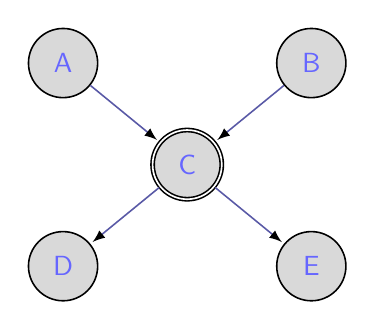
\begin{tikzpicture}[font=\sffamily,node distance=1.cm,->,>=latex,auto,line width=0.2mm]
	
	\tikzset{node st/.style={state,
			fill=gray!30!white,
			text=blue!60!white}}
	\tikzset{node obs/.style={state, draw=none,
			fill=gray!60!black,
			text=blue!20!white}}
	
	\node[node st, accepting] (C) {C};
	\node[above=2em of C] (dumtop) {};
	\node[node st, left=of dumtop] (A) {A};
	\node[node st, right=of dumtop] (B) {B};
	\node[below=2em of C] (dumbot) {};
	\node[node st, left=of dumbot] (D) {D};
	\node[node st, right=of dumbot] (E) {E};
	
	\draw[every loop,
	auto=right,
	draw=blue!30!gray]
	(A) edge [->] node{} (C)
	(B) edge [->] node{} (C)
	(C) edge [->] node{} (D)
	(C) edge [->] node{} (E);	
	\end{tikzpicture}
\end{center}
Answer: $(D \perp E \mid A, B)$, which would not be true by d-separation alone. It only holds because C is a deterministic function of A and B. z




% ======================================================================================
\lecture{Probabilistic Graphical Models}{Template-Based Representations (Ch. 6)}{May 27, 2018}
% ======================================================================================
\vspace{-1.7em}
{\scriptsize Koller and Friedman (2009). Template-Based Representations.\\ \textit{Probabilistic Graphical Models: Principles and Techniques}.\\ }

In what follows, we will build on an example where a vehicle tries to track its true location (L) using various sensor readings: velocity (V), weather (W), failure of sensor (F), observed location (O) of the noisy sensor.
\begin{center}
	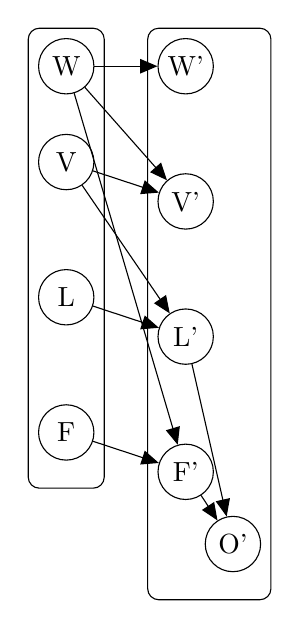
\begin{tikzpicture}[font=\sffamily]
	
	
	% t = 0
	\node[latent] (W) {W};
	\node[latent, below=0.5cm of W] (V) {V};
	\node[latent, below=of V] (L) {L};
	\node[latent, below=of L] (F) {F};
	
	% t = 1
	\node[latent, right=0.8cm of W] (W') {W'};
	\node[latent, below=of W'] (V') {V'};
	\node[latent, below=of V'] (L') {L'};
	\node[latent, below=of L'] (F') {F'};
	\node[latent, below=0.2cm of F', xshift=0.6cm] (O') {O'};
	
	\edge{W} {W',V',F'};
	\edge{V} {V',L'};
	\edge{L} {L'};
	\edge{F} {F'};
	\edge{L',F'} {O'};
	
	\plate {p} 	{(W)(V)(L)(F)} {} ;
	\plate {p2} {(W')(V')(L')(F')(O')} {};
	
	\end{tikzpicture}
\end{center}


\p \blue{Temporal Models}. We discretize time into slices of interval $\Delta$, and denote the ground random variables at time $t \cdot \Delta$ by $\mathcal{X}^{(t)}$. We can simplify our formulation considerably by assuming a \green{Markovian system}: a dynamic system over template variables $\mathcal X$ that satisfies the Markov assumption:
\begin{align}
	(\mathcal{X}^{(t + 1)} \perp \mathcal{X}^{(0:(t-1))} \mid \mathcal{X}^{(t)}) \label{markovian-assumption}
\end{align}
which allows us to define a more compact representation of the joint distribution from time 0 to T:
\begin{align}
	P(\mathcal{X}^{(0:T)}) &= P(\mathcal{X}^{(0)}) \prod_{t = 0}^{T - 1} P(\mathcal{X}^{(t + 1)}  \mid \mathcal{X}^{(t)} ) 
\end{align}
One last simplifying assumption, to avoid having unique transition probabilities for each time $t$, is to assume a \green{stationary}\footnote{Also called time invariant or homogeneous.} Markovian dynamic system, defined s.t. $P(\mathcal{X}^{(t + 1)} \mid \mathcal{X}^{(t)})$ is the same for all $t$.



\myspace
\p \blue{Dynamic Bayesian Networks} (6.2.2). Above, I've drawn the \green{2-time-slice Bayesian network} (2-TBN) for our location example. A 2-TBN is a conditional BN over $\mathcal{X}'$ given $\mathcal{X}_I$, where $\mathcal{X}_I \subseteq \mathcal{X}$ is a set of \purple{interface variables}\footnote{Interface variables are those variables whose values at time $t$ can have a direct effect on the variables at time $t+1$.}. For each template variable $X_i$, the CPD $P(X'_i \mid Pa_{X_i'})$ is a \green{template factor}. We can use the notion of the 2-TBN to define the more general \green{dynamic Bayesian network}:
\begin{definition}
	A \textbf{dynamic Bayesian network} (DBN) is a pair $\langle \beta_0, \beta_{\rightarrow} \rangle$, where $\beta_0$ is a Bayesian network over $\mathcal{X}^{(0)}$, representing the initial distribution over states, and $\beta_{\rightarrow}$ is a 2-TBN for the process. For any $T \ge 0$, the unrolled Bayesian network is defined such that
	\begin{compactitem}
		\item $p(X_i^{(0)} \mid Pa_{X_i^{(0)}})$ is the same as the CPD for the corresponding $X_i$ in $\beta_0$.
		\item $p(X_i^{(t)} \mid Pa_{X_i^{(t)}})$ (for $t > 0$) is the same as the CPD for the corresponding $X_i'$ in $\beta_{\rightarrow}$.  
	\end{compactitem}
\end{definition}

\myspace
\p \blue{State-Observation Models} (6.2.3). Temporal models that, in addition to the Markov assumption (eq. \ref{markovian-assumption}), model the observation variables at time $t$ as conditionally independent of the entire state sequence given the variables at time $t$:
\begin{align}
	\left( 
		\matr{O}^{(t)} \perp \X^{(0:(t-1))}, \X^{(t+1:\infty)}
		\mid
		\X^{(t)}
	\right)
\end{align}
So basically a 2-TBN with the constraint that observation variables are leaves and only have parents in $\X'$. We now view our probabilistic model as consisting of 2 components: the \textit{transition model} $P(\X' \mid \X)$, and the \textit{observation model} $P(\matr O \mid \X)$. The two main architectures for such models are as follows:
\begin{compactitem}
	\item \green{Hidden Markov Models}. Defined as having a single state variable $S$ and a single observation variable $O$. In practice, the transition model $P(S' \mid S)$ is often assumed to be sparse (many possible transitions having zero probability). In such cases, one usually represents them visually as \purple{probabilistic finite-state automaton}\footnote{FSA use the graphical notation where the nodes are the individual possible values in $Val(S)$, and the directed edges from some $a$ \textit{to} $b$ have weight equal to $P(S'=b \mid S=a)$.}.
	
	\item \green{Linear Dynamical Systems} (LDS) represent a system of one or more real-valued variables that evolve linearly over time, with some Gaussian noise. Such systems are often called \purple{Kalman filters}, after the algorithm used to perform tracking. They can be viewed as a DBN with continuous variables and all dependencies are linear Gaussian\footnote{Linear Gaussian: some var $Z$ pointing to $X$ denotes that $X = \Lambda Z + \text{noise}$, where $\text{noise} \sim \mathcal{N}(\mu_x, \Sigma_x)$.}. A LDS is traditionally represented as a state-observation model, where both state and observation are vector-valued RVs, and the transition/observation models are encoded using matrices. More formally, for $\X^{(t)} \in \R^n, O \in \R^m$:\marginnote{
	$$ Q \in \R^{n \times n} $$ $$ H \in \R^{m \times m} $$}[2em]
	\begin{align}
		P(\X^{(t)} \mid \X^{(t-1)})
			&= \mathcal{N}(A \X^{(t-1)}; Q) \\
		P(O^{(t)} \mid \X^{(t)}) 
			&= \mathcal{N}(H \X^{(t)}; R)
	\end{align}
\end{compactitem}

\myspace
\p \blue{Template Variables and Template Factors} (6.3). It's convenient to view the world as being composed of a set of \green{objects}, which can be divided into a set of mutually exclusive and exhaustive \textit{classes} $\mathcal Q = Q_1, \ldots, Q_k$. Template \green{attributes} have a tuple of \textit{arguments}, each of which is associated with a particular class of objects, which defines the set of objects that can be used to instantiate the argument in a given domain. Template attributes thus provide us with a ``generator'' for RVs in a given probability space. Formally,
\begin{definition}
		An \green{attribute} $A$ is a function $A(U_1, \ldots, U_k)$, whose range is some set $Val(A)$, and where each argument $U_i$ is a typed \green{logical variable} associated with a particular class $Q[U_i]$. The tuple $U_1, ldots, U_k$ is called the \green{argument signature} of the attribute $A$, and denoted $\alpha(A)$. 
\end{definition}

\myspace
\p \blue{Plate Models} (6.4.1). The simplest example of a plate model is shown below. It describes multiple RVs generated from the same distribution $\mathcal D$. 

\begin{center}
	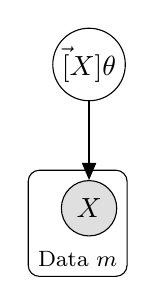
\begin{tikzpicture}[font=\sffamily]
	\node[latent] (theta) {$\vec[X]{\theta}$};
	\node[obs, below=of theta] (X) {$X$};
	
	\edge{theta} {X};
	
	\plate {p} {(X)} {Data $m$} ;
	
	\end{tikzpicture}
\end{center}

This could be a plate model for a set of coin tosses sampled from a single coin. We have a set of $m$ random variables $X(d)$, where $d \in \mathcal D$. Each $X(d)$ is the random variable for the $d$th coin toss. We also explicitly model that the single coin for which the tosses are used is sampled from a distribution $\theta_X$, which takes on values $[0, 1]$ and denotes the bias of the coin. 








% ======================================================================================
\lecture{Probabilistic Graphical Models}{Gaussian Network Models (Ch. 7)}{July 26, 2018}
% ======================================================================================
\vspace{-1.7em}
{\scriptsize Koller and Friedman (2009). Gaussian Network Models.\\ \textit{Probabilistic Graphical Models: Principles and Techniques}.\\ }

\p \blue{Multivariate Gaussians}. Here I'll give two forms of the familiar density function, followed by some comments and terminology.
\begin{align}
	p(\vec x) 
		&= \inv{(2\pi)^{n/2} \sqrt{\det \Sigma}}
			\exp\left\{ 
				-\onehalf (\vec x - \vec\mu)^T \Sigma^{-1} (\vec x - \vec\mu)
			\right\} \\
	p(\vec x) 
		&\propto \exp\left\{ - \onehalf \vec{x}^T J \vec x + (J \vec\mu)^T \vec x  \right\}
		\quad \text{where } J \triangleq \Sigma^{-1}
\end{align}
\begin{compactitem}
	\item The \green{standard Gaussian} is defined as $\mathcal{N}(\vec 0, \matr I)$.
	
	\item $\Sigma$ must be \textit{positive definite}\footnote{Most definitions of p.d. also require that the matrix be symmetric. I also think it helps to view positive definite from the operator perspective: \textit{A linear operator $T$ is positive definite if $T$ is self-adjoint and $\langle T(x), x \rangle > 0$. In other words, ``positive definite'' means that the result of applying the matrix/operator to any nonzero $\vec x$ will always have a positive component along the original direction $\hat{\vec x}$. }}: $\forall \vec x \ne 0, ~ \vec{x}^T \Sigma \vec x > 0$. Recall that $\Sigma_{i,j} = \text{Cov}\left[ x_i, x_j \right] = \E{x_i x_j} - \mu_i \mu_j$.
\end{compactitem}
The two operations we usually want to perform on a Gaussian are (1) computing marginals, and (2) conditioning the distribution on an assignment of some subset of the variables. For (1), its easier to use the standard form of $p(\vec x)$, whereas for (2) it is easier to use the information form (the one using $J$). \\

Multivariate Gaussians are also special because we can easily determine whether two $x_i$ and $x_j$ are independent: $x_i \perp x_j \text{  IFF  } \Sigma_{i,j}=0$\footnote{This is not true in general -- just for multivariate Gaussians!}. For conditional independencies, the information matrix $J$ is easier to work with: $(x_i \perp x_j \mid \{x\}_{k \notin \{i,j\}}) \text{  IFF  } J_{i,j}=0$. This condition is also how we defined pairwise independencies in a Markov network, which leads to the awesome realization:
\begin{definition}
	We can view the information matrix $J$ as directly defining a minimal I-map Markov network for [multivariate Gaussian] $p$, whereby any entry $J_{i,j} \ne 0$ corresponds to an edge $x_i \text{---} x_j$ in the network.
\end{definition}



% ======================================================================================
\lecture{Probabilistic Graphical Models}{Variable Elimination (Ch. 9)}{May 06, 2018}
% ======================================================================================
\vspace{-1.7em}
{\scriptsize Koller and Friedman (2009). Variable Elimination.\\ \textit{Probabilistic Graphical Models: Principles and Techniques}.\\ }

\p \blue{Analysis of Exact Inference}. The focus of this chapter is the conditional probability query,
\begin{align}
	\Prob{\matr Y \mid \matr E = \vec e}
	&= \frac{  \Prob{\matr Y, \vec e}  }{ \Prob{\vec e}  } \tlab{9.1}
\end{align}
Ideally, we want to obtain all instantiations $\Prob{\vec y \mid \vec e}$ of equation \ref{9.1}. Let $\matr W = \mathcal{X} - \matr Y - \matr E$ be the RVs that are neither query nor evidence. Then
\begin{align}
	\Prob{\vec y \mid \vec e} 
	&= \frac { \sum_{\vec w} \Prob{\vec y, \vec e, \vec w}  }{ \sum_{\vec y}  \Prob{\vec y, \vec e} } \tlab{9.3}
\end{align}
and note that, by computing all instantiations for the numerator first, we can reuse them to obtain the denominator. We can formulate the inference problem as a decision problem, which we will call $BNPrDP$, defined as follows\marginnote{$BNPrDP$}[4em]:
\vspace{-0.5em}
\begin{center}
	{\itshape 
	Given: Bayesian network $\mathcal B$ over $\mathcal X$, a variable $X \in \mathcal{X}$, and a value $x \in Val(X)$. \\
	Decide: whether $\Prob[\mathcal B]{X = x} > 0$. 
	}
\end{center}
\purple{Thm 9.1}: The decision problem $BNPrDP$ is $\mathcal{N}\mathcal{P}$-complete. \textbf{Proof}:
\begin{footnotesize}
	\begin{compactenum}
		\item \textbf{BNPrDP is in $\NP$}: Guess a full assignment $\xi$ to the network\footnote{Apparently the time it takes to generate a guess is irrelevant.}. If the guess is successful, where sucess if defined as $(X=x) \in \xi$ and $P(\xi) > 0$, then we know that $P(X=x) > 0$\footnote{This is true because $P(x)$ can be decomposed as $P(\xi) + \sum P(\ldots) \ge P(\xi)$.}. Computing $P(\xi)$ is linear in the number of factors for a BN, since we just multiply them together.
		
		\item \textbf{BNPrDP is $\NP$-hard}. We show this by proving that we can solve 3-SAT (which is $\NP$-hard) by transforming inputs to 3-SAT to inputs of BNPrDP in polynomial time. Given any 3-SAT formula $\phi$, we can create a BN $B_{\phi}$ with some special variable $X$ s.t. $\phi$ is satisfiable IFF $P_{B_{\phi}}(X = x^1) > 0$. You can easily build such a network by having a node $Q_i$ for each binary RV $q_i$, and a node $C_i$ for each of the clauses that's a deterministic function of its parents (up to 3 Q nodes). Then, the node X is a deterministic function of its parents, which are chains of AND gates along the $C_i$. Since each node has at most 3 parents, we can ensure that construction is bounded by polynomial time in the length of $\phi$. 
	\end{compactenum}
\end{footnotesize}

\myspace
\p \blue{Analysis of Approximate Inference}. Consider a specific query $P(\vec y \mid \vec e)$, where we focus on a particular assignment $\vec y$. Let $\rho$ denote some approximate answer, whose accuracy we wish to evaluate relative to the correct probability. We can use the \purple{relative error} to estimate the quality of the approximation: \textit{An estimate $\rho$ has relative error $\epsilon$ if:}
\begin{align}
	\frac{\rho}{1 + \epsilon} \le P(\vec y \mid \vec e) \le \rho (1 + \epsilon)
\end{align}
Unfortunately, the task of finding some approximation $\rho$ with relative error $\epsilon$ \textit{is also $\NP$-hard}. Furthermore, even if we relax this metric by using absolute error instead, we end up finding that \textbf{in the case where we have evidence, approximate inference is no easier than exact inference, in the worst case}.

\myspace
\p \blue{Variable Elimination}. Basically, a dynamic programming approach for performing exact inference. Consider the simple BN $X_1 \rightarrow \cdots \rightarrow X_n$, where each variable can take on $k$ possible values. The dynamic programming approach for computing $P(X_{n})$ involves computing
\begin{align}
	P(X_{i + 1}) = \sum_{x_i} P(X_{i + 1} \mid x_i) P(x_i)
\end{align} 
$n - 1$ times, starting with $i = 1$, all the way up to $i = n - 1$, reusing the previous computation at each step, with total cost $\mathcal{O}(nk^2)$. So for this simple network, even though the size of the joint is $k^n$ (exponential in $n$), we can do inference in linear time. 

First, we formalize some basic concepts before defining the algorithm. 

\p \textbf{Factor marginalization}:
\vspace{-1em}
\begin{quote}
	{\itshape
		Let $\matr X$ be a set of variables, and $Y \notin \matr X$ a variable. Let $\phi(\matr X, Y)$ be a factor. Define the \green{factor marginalization} of $Y$ in $\phi$, denoted $\sum_Y \phi$, to be a factor $\psi$ over $\matr X$ such that:
		$$
		\psi(\matr X) = \sum_Y \phi(\matr X, Y)
		$$	
	}
\end{quote} 
The key observation that's easy to miss is that \textit{we're only summing entries in the table where the values of $\X$ match up}. One useful rule for exchanging factor product and summation: If $X \notin Scope[\phi_1]$, then
\begin{align}
	\sum_X (\phi_1 \cdot \phi_2) = \phi_1 \cdot \sum_X \phi_2 \tlab{9.6}
\end{align}

\Needspace{10\baselineskip}
So, when computing some marginal probability, the main idea is to group factors together and compute expressions of the form
\graybox{
	\sum_{\Z} \prod_{\phi \in \Phi} \phi
} where $\Phi$ is the set of all factors $\phi$ for which $\Z \in Scope[\phi]$. This is commonly called the \green{sum-product} inference task. The full algorithm for sum-product variable elimination, which is an instantiation of the sum-product inference task, is illustrated below.

\myfig[0.4\textwidth]{figs/variable_elimination.png}

This is what we use to compute the marginal probability $P(\X)$ where $\X = \mathcal{X} - \Z$. To compute conditional queries of the form $P(\Y \mid \matr{E} = \vec e)$, simply replace all factors whose scope overlaps with $\matr E$ with their reduced factor (see chapter 4 notes for definition) to get the unnormalized $\phi^*(\Y)$ (the numerator of $P(\Y \mid \vec e)$). Then divide by $\sum_{\vec y} \phi^*$ to obtain the final result.


\myspace
\p \blue{Example}. We will work through computing $P(Job)$ for the BN below. 

\begin{center}
	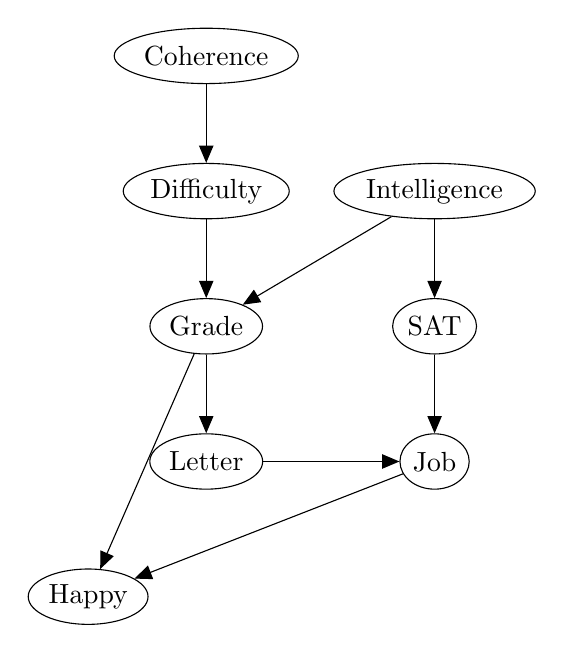
\begin{tikzpicture}[font=\sffamily]
	
	\node[latent, ellipse] (C) 								{Coherence};
	\node[latent, ellipse, below=of C] (D) 					{Difficulty};
	\node[latent, ellipse, below=of C, xshift=2.9cm] (I)	{Intelligence};
	
	\node[latent, ellipse, below=of D] (G) 	{Grade}; 
	\node[latent, ellipse, below=of I] (S) 	{SAT};
	
	\node[latent, ellipse, below=of G] (L) 					{Letter};
	\node[latent, ellipse, below=1cm of S] (J) 				{Job};
	\node[latent, ellipse, below=of L, xshift=-1.5cm] (H) 	{Happy};
	
	\edge{C} {D};
	\edge{D} {G};
	\edge{I} {G, S};
	\edge{S} {J};
	\edge{G} {L, H};
	\edge{L} {J};
	\edge{J} {H};
	\end{tikzpicture}
\end{center}

\p Due to Happy being a child of Job, $P(J)$ actually requires using all factors in the graph. Below shows how VE with elimination ordering $C,D,I,H,G,S,L$ progressively simplifies the equation for computing $P(J)$. 
\begin{align}
	P(J) &= \sum P(J \mid s, \ell) P(s \mid i) P(\ell \mid g) P(g \mid d, i) P(d \mid c) P(h \mid J, g) P(c) P(i) \\
	&= \sum_{\mred{c},d, i, h, g, s, \ell} \mred{(P(c) P(d \mid c) )} \cdot
		P(g \mid d, i) 
		P(i) P(s \mid i) 
		P(h \mid J, g) P(\ell \mid g) 
		P(J \mid s, \ell) \\
	&= \sum_{\mred{d},i, h, g, s, \ell} \mred{ (\tau_1(d) P(g \mid d, i)) }\cdot
		P(i)P(s \mid i)
		P(h \mid J, g) P(\ell \mid g)
		P(J \mid s, \ell) \\
	&= \sum_{\mred{i}, h, g, s, \ell} \mred{( \tau_2(g, i) P(i) P(s \mid i))} \cdot
		P(h \mid J, g)P(\ell \mid g) 
		P(J \mid s, \ell) \\	
	&= \sum_{\mred{h}, g, s, \ell} \mred{( P(h \mid J, g) )}  \cdot
		\tau_3(g, s) P(\ell \mid g) 
		P(J \mid s, \ell) \\	
	&= \sum_{\mred{g},s, \ell} \mred{(\tau_4(g, J) \tau_3(g, s) P(\ell \mid g) )} \cdot  
		P(J \mid s, \ell) \\	
	&= \sum_{ \mred{s},\ell} \mred{\tau_5(J, \ell, s) \cdot P(J \mid s, \ell)} \\
	&= \sum_{\mred{\ell}} \mred{\tau_6(J, \ell) }
\end{align}
where red indicates the focus of the given step in the VE algorithm.

\clearpage
% ======================================================================================
\lecture{Probabilistic Graphical Models}{Clique Trees (Ch. 10)}{May 06, 2018}
% ======================================================================================
\vspace{-1.7em}
{\scriptsize Koller and Friedman (2009). Clique Trees.\\ \textit{Probabilistic Graphical Models: Principles and Techniques}.\\ }

\p \blue{Cluster Graphs}. A graphical flowchart of the factor-manipulation process that will be relevant when we discuss message passing. Each node is a \textit{cluster}, which is associated with a subset of variables. Formally,
\vspace{-0.7em}
\begin{quote}
	{\itshape A \green{cluster graph} $\mathcal{U}$ for a set of factors $\Phi$ over $\mathcal X$ is an undirected graph. Each node $i$ is associated with a subset $\matr[i]{C} \subseteq \mathcal X$. Each factor $\phi \in \Phi$ must be associated with a cluster $\matr[i]{C}$, denoted $\alpha(\phi)$, such that $Scope[\phi] \subseteq \matr[i]{C}$ (\green{family-preserving}). Each edge between a pair of clusters $\matr[i]{C}$ and $\matr[j]{C}$ is associated with a \purple{sepset} $\matr[i,j]{S} \subseteq \matr[i]{C} \cap \matr[j]{C}$.  }
\end{quote}
Recall that each step of variable elimination involves creating a factor $\psi_i$ by multiplying a group of factors\footnote{All whose scope contains the variable we are currently trying to eliminate.}. Then, denoting the variable we are eliminating at this step as $Z$, we obtain another factor $\tau_i$ that's the factor marginalization of $Z$ in $\psi_i$ (denoted $\sum_Z \psi_i$). An execution of variable elimination defines a cluster graph: we have a cluster for each of the $\psi_i$, defined as $\matr[i]{C} = Scope[\psi_i]$. We draw an edge between $\matr[i]{C}$ and $\matr[j]{C}$ if the \green{message} $\tau_i$ is used in the computation of $\tau_j$. \\

Consider when we applied variable elimination to the student graph network below, to compute $P(J)$. Elimination ordering $C,D,I,H,G,S,L$.

\begin{center}
	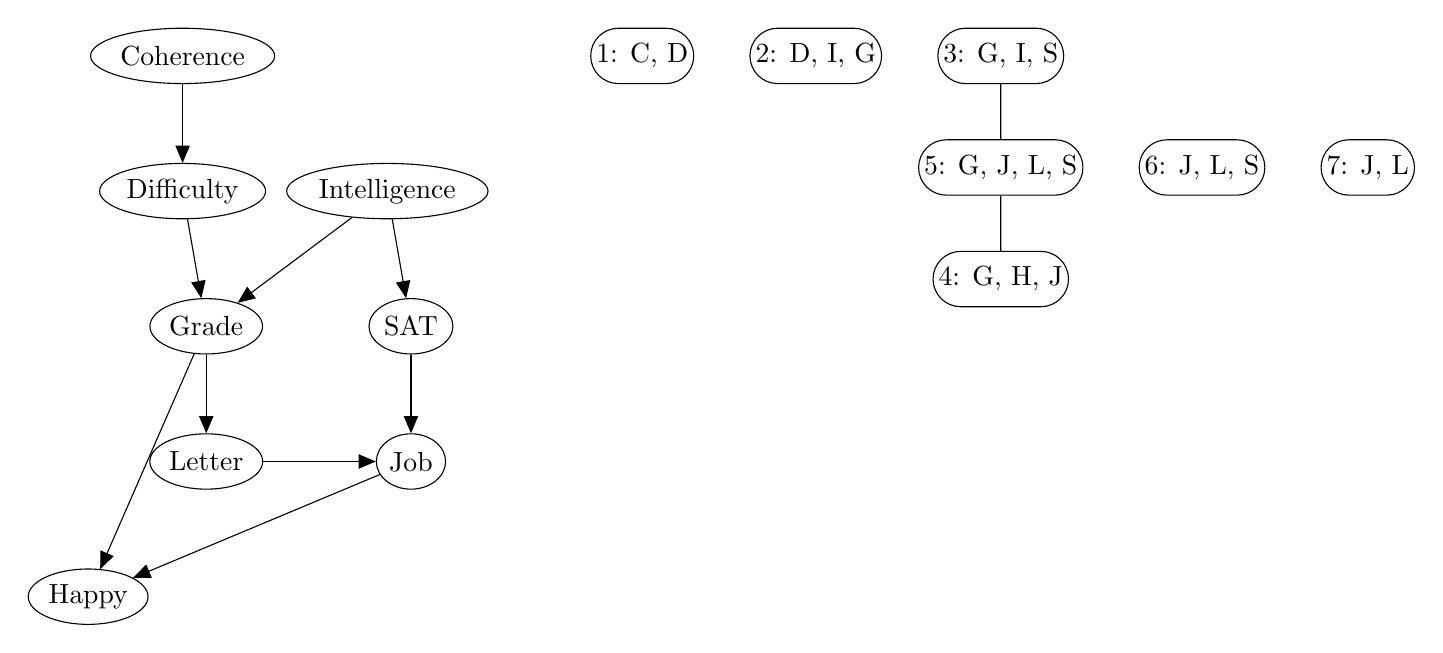
\begin{tikzpicture}[font=\sffamily]
	
	\node[latent, ellipse] (C) {Coherence};
	\node[latent, ellipse, below=of C] (D) {Difficulty};asf
	\node[latent, ellipse, below=of C, xshift=2.6cm] (I) {Intelligence};
	
	\node[latent, ellipse, below=of D, xshift=0.3cm] (G) {Grade}; 
	\node[latent, ellipse, below=of I, xshift=0.3cm] (S) {SAT};
	
	\node[latent, ellipse, below=of G] (L) {Letter};
	\node[latent, ellipse, below=1cm of S] (J) {Job};
	\node[latent, ellipse, below=of L, xshift=-1.5cm] (H) {Happy};
	
	\edge{C} {D};
	\edge{D} {G};
	\edge{I} {G, S};
	\edge{S} {J};
	\edge{G} {L, H};
	\edge{L} {J};
	\edge{J} {H};
	
	
	\node[latent, rounded rectangle, right=4cm of C] 	(CD) 	{1: C, D};
	\node[latent, rounded rectangle, right=0.7cm of CD]  		(DIG) 	{2: D, I, G};
	\node[latent, rounded rectangle, right=0.7cm of DIG]		(GIS) 	{3: G, I, S};
	\node[latent, rounded rectangle, below=0.7cm of GIS]		(GJLS) 	{5: G, J, L, S};
	\node[latent, rounded rectangle, below=0.7cm of GJLS]		(GHJ) 	{4: G, H, J};
	\node[latent, rounded rectangle, right=0.7cm of GJLS]		(JLS) 	{6: J, L, S};
	\node[latent, rounded rectangle, right=0.7cm of JLS]		(JL) 	{7: J, L};
	
	\medge[-] {CD} 		{DIG} {D};
	\medge[-] {DIG} 	{GIS} {G,I};
	\edge[-] {GIS, GHJ}	{GJLS};
	\medge[-] {GJLS} {JLS} {J,S,L};
	\medge[-] {JLS} {JL} {J,L};
	\end{tikzpicture}
\end{center}

\myspace
\p \blue{Clique Trees}. Since VE uses each intermediate $\tau_i$ at most once, the cluster graph induced by an execution VE is necessarily a \textit{tree}, and it also defines a directionality: the direction of the message passing (left-to-right in the above illustration). All the messages flow toward a single cluster where the final result is computed -- the \textbf{root} of the tree; we say the messages ``flow up'' to the root. Furthermore, for cluster trees induced by VE, the scope of each message (edge) $\tau_i$ is \textit{exactly} $\matr[i]{C} \cap \matr[j]{C}$, not just a subset\footnote{This follows from the \green{running intersection property}, which is satisfied by any cluster tree that's defined by variable elimination. It's defined as, if any variable $X$ is in both cluster $\matr[i]{C}$ and $\matr[j]{C}$, then $X$ is also in every cluster in the (unique) path in the tree between $\matr[i]{C}$ and $\matr[j]{C}$.}.
\vspace{-0.7em}
\begin{quote}
	{\itshape Let $\Phi$ be a set of factors over $\mathcal X$. A cluster tree over $\Phi$ that satisfies the running intersection property is called a \green{clique tree}. For clique trees, the clusters are also called \green{cliques}. }
\end{quote}


\myspace
\p \blue{Message Passing: Sum Product}. Previously we saw how an execution of VE can be illustrated with a clique tree. We now go the other direction -- given a clique tree, we show how it can be used for variable elimination. Given a clique tree representation of some BN, we can use it to guide us along an execution of VE to compute any marginal we'd like. First, before any run, we generate the set of \green{initial potentials} $\psi_i$ associated with each clique $\matr[i]{C}$ in the tree, defined as just the multiplication of the initial factors associated with the clique. We define the root of the tree as any clique containing the variable whose marginal we want to compute (we pick arbitrarily). Starting from the leaves and moving toward the root, we pass messages along from clique to clique. A clique is \textit{ready} to send a message when it has received a message from all of its downstream neighbors. The message from $\matr[i]{C}$ to [a neighbor] $\matr[j]{C}$ is computed using the \green{sum-product message passing} computation:
\graybox{
	\delta_{i \rightarrow j} &= \sum_{ \matr[i]{C} - \matr[i,j]{S}  }	\psi_i \cdot \prod_{k \in ( Nb_i - \{j\}   )} \delta_{k \rightarrow i} \tlab{10.2}
}
where the summation is simply over the variables in $\matr[i]{C}$ that aren't passed along to $\matr[j]{C}$, and the product is over all messages that $\matr[i]{C}$ received. Stated even simpler, we multiply all the incoming messages by our initial potential, then sum out all variables except those in $\matr[i,j]{S}$. When the root clique has received all messages, it multiplies them with its own initial potential, resulting in a factor called the \green{beliefs}, $\beta_r(\matr[r]{C})$. It represents
\begin{align}
	\widetilde{P}_{\Phi}(\matr[r]{C}) = \sum_{\mathcal X - \matr[r]{C}} \prod_{\phi} \phi
\end{align}
where, to be clear, the product is over all $\phi$ in the graph. \\

\p Below is a more compact summary of all of this, showing the procedure for computing \textit{all} final factors (belief) $\beta_i$ for some marginal probability query on the variables in $\matr[r]{C}$ \textit{asynchronously}. \\ 
\purple{Algorithm 10.2: Sum-Product Belief Propagation}
\begin{compactenum}
	\item For each clique $\matr[i]{C}$, compute its initial potential:
	$$
		\psi_i(\matr[i]{C}) \leftarrow \prod_{\phi_j : \alpha(\phi_j)=i }\big[  \phi_j  \big]
	$$
	
	\item While $\exists i,j$ such that $i$ is ready to transmit to $j$, compute:
	$$
		\delta_{i \rightarrow j} \leftarrow \sum_{ \matr[i]{C} - \matr[i,j]{S}  }	\psi_i \cdot \prod_{k \in ( Nb_i - \{j\}   )} \delta_{k \rightarrow i}
	$$
	
	\item Then, compute each belief factors $\beta_i$ by multiplying the initial potential $\psi_i$ by the incoming messages to $\matr[i]{C}$:
	$$
		\beta_i \leftarrow \psi_i \cdot \prod_{k \in Nb_{C_i}} \delta_{k \rightarrow i}
	$$
	
	\item Return the set of beliefs $\{ \beta_i \}$, where 
	\begin{align}
		\beta_i = \sum_{\mathcal{X} - \matr[i]{C}} \widetilde{P}_{\Phi}(\mathcal{X}) =  \widetilde{P}_{\Phi}(\matr[i]{C})
	\end{align}
\end{compactenum}
The SP Belief Propagation algorithm above is also called \green{clique tree calibration}. A clique tree $\mathcal{T}$ is \textit{calibrated} if all pairs of adjacent cliques are calibrated. A calibrated clique tree satisfies the following property for what we'll now call the \green{clique beliefs}, $\beta_i$, and the \green{sepset beliefs}, $\mu_{i,j}$ over $\matr[i,j]{S}$:\marginnote{$\mu_{i,j} = \widetilde{P}_{\Phi}(\matr[i,j]{S})$}[3em]
\graybox{
	\mu_{i,j}(\matr[i,j]{S}) \triangleq \sum_{\matr[i]{C} - \matr[i,j]{S}} \beta_i  &= \sum_{\matr[j]{C} - \matr[i,j]{S}} \beta_j 
}
\vspace{-0.5em}
\begin{quote}
	{\itshape\small
	The main advantage of the clique tree algorithm is that it computes the posterior probability of all variables in a graphical model using only twice the computation\footnote{The algorithm is equivalent to doing one upward pass, one downward pass.} of the upward pass in the same tree. 
	}
\end{quote}
We can also show that $\mu_{i,j} = \delta_{j \rightarrow i} \delta_{i \rightarrow j}$, which then allows us to derive:
\begin{align}
	\widetilde{P}_{\Phi}(\mathcal X) &= \dfrac{ \prod_{i \in \mathcal{V}_{\mathcal T}} \beta_i
		}{  \prod_{ij \in \mathcal{E}_{\mathcal T}} \mu_{i,j}  } 
	\tlab{10.10}
\end{align}
In other words, the clique and sepset beliefs provide a \green{reparameterization} of the unnormalized measure, a property called the \green{clique tree invariant}.

\myspace
\p \blue{Message Passing: Belief Update}. We know discuss an alternative message passing approach that is mathematically equivalent but intuitively different than the sum-product approach. First, we introduce some new definitions.

\p \textbf{Factor Division}:\marginnote{Define 0/0 = 0}[3em]
\vspace{-1em}
\begin{quote}
	{\itshape Let $\X$ and $\Y$ be disjoint sets of variables, and let $\phi_1(\X, \Y)$ and $\phi_2(\Y)$ be two factors. We define the division of $\phi_1$ and $\phi_2$ as a factor $\psi$ with scope $\X, \Y$ as follows:
		$$
		\psi(\X, \Y) \triangleq \frac{  \phi_1(\X, \Y)  }{  \phi_2(\matr Y)}
		$$
	}
\end{quote}
Looking back at equation \ref{10.2}, we can now see that another way to write $\delta_{i \rightarrow j}$ is
\begin{align}
	\delta_{i \rightarrow j} = \frac{ \sum_{\matr[i]{C} - \matr[i,j]{S}} \beta_i }{ \delta_{j \rightarrow i} } \tlab{10.13}
\end{align}
Now, consider the clique tree below for the simple Markov network A-B-C-D:
\vspace{-0.5em}
\begin{center}
	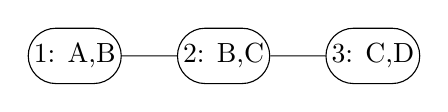
\begin{tikzpicture}[font=\sffamily]
	
	\node[latent, rounded rectangle] 							(AB) 	{1: A,B};
	\node[latent, rounded rectangle, right=0.7cm of AB]  		(BC) 	{2: B,C};
	\node[latent, rounded rectangle, right=0.7cm of BC]		(CD) 	{3: C,D};
	
	\edge[-] {AB} 		{BC};
	\edge[-] {BC} 		{CD};
	\end{tikzpicture}
\end{center}
\vspace{-0.5em}
If we assigned $\matr[2]{C}$ as the root, then our previous approach would compute $\delta_{2 \rightarrow 1}$ as $\sum_C \psi_2 \cdot \delta_{3 \rightarrow 2}$. Alternatively, we can use equation \ref{10.13} to realize this is equivalent to dividing $\beta_2$ by $\delta_{1 \rightarrow 2}$ and marginalizing out $C$. This observation motivates the algorithm below, which allows us to execute message passing in terms of the clique and sepset beliefs, without having to remember the initial potentials $\psi_i$ or explicitly compute the messages $\delta_{i \rightarrow j}$. 

\purple{Algorithm 10.3: Belief-Update Message Passing}
\begin{compactenum}
	\item For each clique $\matr[i]{C}$, set its initial belief $\beta_i$ to its initial potential $\psi_i$. For each edge in $\mathcal{E}_{\mathcal T}$, set $\mu_{i,j} = \mathbf{1}$.
	
	\item Wile there exists an uninformed\footnote{A clique is informed once it has received informed messages from all of its neighbors. An informed message is one that has been sent by taking into account information from all of the sending cliques' neighbors (aside from the receiving clique of that message, of course).} clique in $\mathcal T$, select any edge in $\mathcal{E}_{\mathcal T}$, and compute
	\graybox{
		\sigma_{i \rightarrow j} &\leftarrow \sum_{ \matr[i]{C} - \matr[i,j]{S} } \big[  \beta_i \big] \\
		\beta_j &\leftarrow \beta_j \cdot \frac{ \sigma_{i \rightarrow j} }{  \mu_{i,j}  } \\
		\mu_{i,j} &\leftarrow \sigma_{i \rightarrow j}
	}
	
	\item Return the resulting set of informed beliefs $\{ \beta_i \}$. 
\end{compactenum}
At convergence, $\sigma_{i \rightarrow j} = \mu_{i,j} = \sigma_{j \rightarrow i}$. 









% ======================================================================================
\lecture{Probabilistic Graphical Models}{Inference as Optimization (Ch. 11)}{June 02, 2018}
% ======================================================================================
\vspace{-1.7em}
{\scriptsize Koller and Friedman (2009). Inference as Optimization.\\ \textit{Probabilistic Graphical Models: Principles and Techniques}.\\ }

\p \blue{Propagation-Based Approximation}. We can use a general-purpose cluster graph rather than the more restrictive clique tree (needed to guarantee exact inference) for approximate inference methods. Consider the simple Markov network below on the left.


\begin{center}
	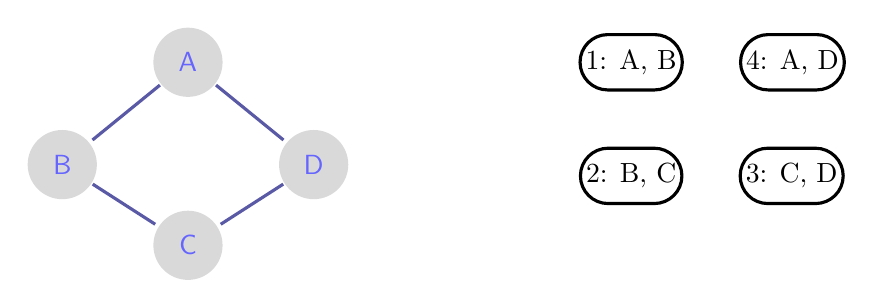
\begin{tikzpicture}[font=\sffamily,node distance=1.cm,->,>=latex,auto,line width=0.4mm]
	
	
	\tikzset{node st/.style={state, draw=none,
			fill=gray!30!white,
			text=blue!60!white}}
	\tikzset{node obs/.style={state, draw=none,
			fill=gray!60!black,
			text=blue!20!white}}
	
	\node[node st] (A) {A};
	\node[below=2em of A] (dummy) {};
	\node[node st, left=of dummy] (D) {B};
	\node[node st, right=of dummy] (B) {D};  
	\node[node st, below=4em of A] (C) {C};
	
	\draw[every loop,
	auto=right,
	draw=blue!30!gray]
	(A) edge[-] node{} (B)
	(A) edge[-] node{} (D)
	(B) edge[-] node{} (C)
	(D) edge[-] node{} (C);
	
	
	
	\node[latent, rounded rectangle, right=4.5cm of A] 	(AB) 	{1: A, B};
	\node[latent, rounded rectangle, right=0.7cm of AB] (AD) 	{4: A, D};
	\node[latent, rounded rectangle, below=0.7cm of AB] (BC) 	{2: B, C};
	\node[latent, rounded rectangle, right=0.7cm of BC] (CD) 	{3: C, D};

	
	\medge[-] {AB} 		{AD} {A};
	\medge[-] {AB}		{BC} {\hspace*{-0.2cm}B};
	\medge[-] {BC} 		{CD} {C};
	\medge[-] {AD} 		{CD} {\hspace*{0.2cm}D}
	\end{tikzpicture}
\end{center}

The clique tree for this network, which can be used for exact inference, has two cliques ABD and BCD and messages are passed between them consisting of $\tau(B, D)$. Suppose that, instead, we set up 4 clusters corresponding to each of the initial potentials, shown as the cluster graph above on the right. We can still apply belief propagation here, but due to it now having loops (as opposed to before when we only had trees), \textit{the process may not converge}. 













% ======================================================================================
\lecture{Probabilistic Graphical Models}{Parameter Estimation (Ch. 17)}{June 17, 2018}
% ======================================================================================
\vspace{-1.7em}
{\scriptsize Koller and Friedman (2009). Parameter Estimation.\\ \textit{Probabilistic Graphical Models: Principles and Techniques}.\\ }

\p \blue{Maximum Likelihood Estimation} (17.1). In this chapter, assume the network structure is fixed and that our data set $\mathcal D$ consists of fully observed instances of the network variables: $\mathcal D = \{ \xi[1], \ldots, \xi[M] \}$. We begin with the simplest learning problem: parameter learning for a single variable. We want to estimate the probability, denoted via the \textit{parameter} $\theta$, with which the flip of a thumbtack will land heads or tails. Define the \green{likelihood function} $L(\theta : \vec{x})$ as the probability of observing some sequence of outcomes $\vec{x}$ under the parameter $\theta$. In other words, it is simply $P(\vec x : \theta)$, but interpreted as a \textit{function of $\theta$}. For our simple case, where $\mathcal D$ consists of $M$ thumbtack flip outcomes,
\begin{align}
	L(\theta : \mathcal D) &= \theta^{M[1]} (1 - \theta)^{M[0]}
\end{align}
where $M[1]$ denotes the number of outcomes in $\mathcal D$ that were heads. Since it's easier to maximize a logarithm, and since it yields the same optimal $\hat \theta$, optimize the \green{log-likelihood} to obtain:
\begin{align}
	\hat \theta &= \argmax_{\theta} \ell (\theta : \mathcal D) = \argmax_{\theta} \big[ M[1] \log\theta + M[0]\log(1 - \theta) \big] \\
	&= \frac{ M[1] }{ M[1] + M[0] }
\end{align}
Note that MLE has the \textit{disadvantage} that it can't communicate confidence of an estimate\footnote{We get the same result (0.3) if we get 3 heads out of 10 flips, as we do for getting 300 heads out of 1000 flips; yet, the latter experiment should include a higher degree of confidence}. \\

We now provide the more general formal definitions for MLE. 
\begin{compactitem}
	\item We are given a \textit{training set} $\mathcal D$ containing $M$ (IID) instances of a set of random variables $\mathcal X$, where the samples of $\mathcal X$ are drawn from some unknown distribution $P^*(\mathcal X)$. 
	
	\item We are given a \green{parametric model}, defined by a function $P(\xi ; \vec{\theta})$, where $\xi$ is an instance of $\mathcal X$, and we want to estimate its parameters $\vec{\theta}$\footnote{We also have the constraint that $P(\xi ; \vec{\theta})$ must be a valid distribution (nonnegative and sums to 1 over all possible $\xi$)}. The model also defines the space of legal parameter values $\Theta$, the \green{parameter space}. 
	
	\item We then define the \green{likelihood function} $L(\vec{\theta} : \mathcal D) = \prod_m P(\xi[m] : \vec{\theta})$. 
\end{compactitem}

\p We can often simplify the likelihood function to simpler terms, like our $M[0]$ and $M[1]$ values in the thumbtack example. These are called the \green{sufficient statistics}, defined as functions of the data that summarize the relevant information for computing the likelihood. Formally,
\vspace{-0.5em}
\begin{quote}
	{\small\itshape 
		A function $\tau(\xi) : \xi \rightarrow \R^{\ell}$ (for some $\ell$) is a \green{sufficient statistic} if for any two data sets $\mathcal D$ and $\mathcal{D}'$, we have that
		\graybox{
			\bigg[ \sum_{ \xi[m] \in \mathcal D } \tau(\xi[m])	 = \sum_{ \xi'[m] \in \mathcal D' } \tau(\xi'[m]) \bigg]
			\implies 
			\bigg[ L(\vec{\theta} : \mathcal D) = L(\vec{\theta} : \mathcal D')    \bigg]
		} 
		\textbf{We often informally refer to the tuple $\sum_{\xi[m] \in mathcal D} \tau(\xi[m])$ as the sufficient statistics of the data set $\mathcal D$.}
	}
\end{quote}

\myspace
\p \blue{MLE for Bayesian Networks -- Simple Example}. We now move on to estimating parameters $\vec{\theta}$ for the simple BN $X \rightarrow Y$ for two binary RVs $X$ and $Y$. Our parameters $\vec{\theta}$ are the individual probabilities of $P(X)$ and $P(Y \mid X)$ (6 total). Since BNs have the nice property that their joint probability decomposes into a product of probabilities, just like how the likelihood function is a product of probabilities, we can write the likelihood function as a product of the individual \textit{local} probabilities:\marginnote{decomposability of the likelihood function}[2em]
\begin{align}
	L(\vec{\theta} : \mathcal D) &= \bigg( \prod_m P(x[m] : \vec[X]{\theta})  \bigg) \bigg( \prod_m P(y[m] \mid x[m] : \vec[Y \mid X]{\theta}) \bigg)
\end{align}
which can be decomposed even further by e.g. differentiating products over $x[m]:x[m]=x^0$ etc. Just as we used $M[0]$ in the thumbtack example to count the number of instances with a certain value, we can use the same idea for the general case. 
\vspace{-0.5em}% TODO: 19.{1.1, 1.3, 2.2}
\begin{quote}
	{\small\itshape
		Let $\Z$ be some set of RVs, and $\vec{z}$ be some instantiation to them. We define $M[\vec{z}]$ to be the number of entries in data set $\mathcal D$ that have $\Z[m] = \vec{z}$:
		\begin{align}
			M[\vec z] &= \sum_m \ind\{\Z[m] = \vec z \}
		\end{align}
	}
\end{quote}


\myspace
\p \blue{Global Likelihood Decomposition}. We now move to the more general case of computing the likelihood for BN with structure $\mathcal G$.\marginnote{global decomposition of the likelihood}[2em]
\begin{align}
	L(\vec{\theta} : \mathcal D) &= \prod_m P_{\mathcal G} (\xi[m] : \vec{\theta}) \\
	&= \prod_m \prod_i P(x_i[m] \mid Pa_{X_i}[m] : \vec{\theta}) \\
	&= \prod_i \bigg[ \prod_m  P(x_i[m] \mid Pa_{X_i}[m] : \vec[X_i \mid Pa_{X_i}]{\theta})  \bigg] \\
	&= \prod_i L_i (\vec[X_i \mid Pa_{X_i}]{\theta} : \mathcal D)
\end{align}
where $L_i$ is the \green{local likelihood function} for $X_i$. Assuming these are each disjoint sets of parameters from one another, it implies that $\hat{\vec{\theta}} = \langle \vec[X_1 \mid Pa_{X_1}]{\hat{\theta}}, \ldots, \vec[X_n \mid Pa_{X_n}]{\hat{\theta}}   \rangle$







% ======================================================================================
\lecture{Probabilistic Graphical Models}{Partially Observed Data (Ch. 19)}{June 17, 2018}
% ======================================================================================
\vspace{-1.7em}
{\scriptsize Koller and Friedman (2009). Partially Observed Data.\\ \textit{Probabilistic Graphical Models: Principles and Techniques}.\\ }

\p \blue{Likelihood of Data and Observation Models} (19.1.1). Consider the simple example of flipping a thumbtack, but occasionally the thumbtack rolls off the table. We choose to ignore the tosses for which the thumbtack rolls off. Now, in addition to the random variable $X$ giving the flip outcome, we have the \textit{observation variable} $O_X$, which tells us whether we observed the value of X. 
\begin{center}
	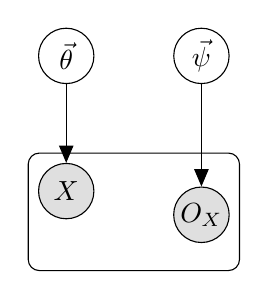
\begin{tikzpicture}[font=\sffamily]
	\node[latent] (theta) {$\vec{\theta}$};
	\node[obs, below=of theta] (X) {$X$};
	\edge{theta} {X};
	
	\node[latent, right=of theta] (psi) {$\vec\psi$};
	\node[obs, below=1.3cm of psi] (OX) {$O_X$};
	\edge{psi} {OX};
	
	\plate {p} {(X)(OX)} {} ;
	\end{tikzpicture}
\end{center}
The illustration above is a plate model where we choose a thumbtack sampled with bias $\vec{\theta}$ and repeat some number of flips with that same thumbtack. We also sample the random variable $O_X$ that has probability of observation sampled from $\psi$ and fixed for all the experiments we do. This leads to the following definition for the observability model. 
\vspace{-0.5em}
\begin{quote}
	{\small\itshape
		Let $\X = \{X_1, \ldots X_n \}$ be some set of RVs, and let $O_{\X} = \{ O_{X_1}, \ldots, O_{X_n}  \}$ be their \green{observability variable}. The \green{observability model} is a join distribution $$P_{missing}(\X, O_{\X}) = P(\X) \cdot P_{missing}(O_{\X} \mid \X)$$so that $P(\X)$ is parameterized by $\vec{\theta}$ and $P_{missing}(O_{\X} \mid \X)$ is parameterized by $\vec{\psi}$. We define a new set of RVs $\Y = \{Y_1, \ldots Y_n \}$ where $Val(Y_i) = Val(X_i) \cup \{?\}$. The actual observation $\Y$ is a deterministic function of $\X$ and $O_{\X}$:
		\begin{align}
			Y_i = \begin{cases}
				X_i & O_{X_i} = o^1 \\
				? & O_{X_i} = o^0
			\end{cases}
		\end{align}
	}
\end{quote}
For our simple model above, we have
\begin{align}
	P(Y = 1) &= \theta \psi \\
	P(Y = 0) &= (1 - \theta) \psi \\
	P(Y = ?) &= (1 - \psi) \\
	L(\theta, \psi; \mathcal D) &= \theta^{M[1]}(1 - \theta)^{M[0]}\psi^{M[1] + M[0]} (1 - \psi)^{M[?]}
\end{align}
The main takeaway is to understand that \textbf{when we have missing data, the data-generation process involves two steps: (1) generate data by sampling from the model, then (2) determine which values we get to observe and which ones are hidden from us}. 


\myspace \p \blue{The Likelihood Function} (19.1.3). Assume we have a BN network $\mathcal G$ over a set of variables $\X$. In general, each instance has a different set of observed variables. Denote by $\matr{O}[m]$ and $\vec{o}[m]$ the observed vars and their values in the $m$'th instance, and by $\matr{H}[m]$ the missing (or hidden) vars in the $m$'th instance. 

% \myspace \p \blue{Expectation Maximization (EM)} (19.2.2). 









\renewcommand{\Z}{\mathbb{Z}}
% ==================================================================================
% ==================================================================================
% ==================================================================================
% ITILA
% ==================================================================================
% ==================================================================================
% ==================================================================================
\mysection{Information Theory, Inference, and Learning Algorithms}\label{Information Theory, Inference, and Learning Algorithms}


% ======================================================================================
\lecture{Information Theory, Inference, and Learning Algorithms}{Introduction to Information Theory (Ch. 1)}{November 11, 2017}
% ======================================================================================

{\footnotesize [Note: Skipping most of this chapter since it's mostly introductory material.]}

\p \blue{Preface}. For ease of reference, some common quantities we will frequently be using: 
\begin{compactitem}
	\item \textbf{Binomial distribution}. Let $r$ denote the number of successful trials out of $N$ total trials. Let $f$ denote the probability of success for a single trial.
	\begin{align}
	\Prob{r \mid f, N} = \binom{N}{r} f^r (1 - f)^{N - r} \qquad
	\E{r} = Nf \qquad
	\Var{r} = Nf(1-f)
	\end{align}
	
	\item \textbf{Stirling's Approximation}.\marginnote{Recall that $\log_b x = \frac{\log_a x}{\log_a b}$}[2em]
	\begin{align}
	x! \simeq x^x e^{-x} \sqrt{2 \pi x} 
	\quad &\Leftrightarrow \quad
	\ln x! \simeq x \ln x - x + \onehalf \ln 2 \pi x \\
	\ln\binom{N}{r} &\simeq r \ln \frac{N}{r} + (N - r) \ln \frac{N}{N - r}
	\end{align}
	
	\item \textbf{Binary Entropy Function} and its relation with Stirling's approximation.
	\begin{align}
	H_2(x) &\triangleq x \lg \inv{x} + (1-x) \lg \inv{1 - x} \\
	\lg \binom{N}{r} &\simeq N H_2(r/N)
	\end{align}
\end{compactitem}

\Needspace{25\baselineskip}
\bluesec{Perfect communication over an imperfect, noisy communication channel (1.1)}. We want to make an encoder-decoder architecture, of the general form in the figure below, to achieve reliable communication over a noisy channel.
\myfig[0.55\textwidth]{ITILA_1_6.png} 

\green{Information theory} is concerned with the theoretical limitations and potentials of such systems. Let's explore some examples for the case of the \green{binary symmetric channel}\footnote{A binary symmetric channel transmits each bit correctly with probability (1 - f) and incorrectly with probability f, \textbf{where $f$ is assumed to be small.}}:
\begin{compactitem}
	\item \textbf{Repetition codes}. Let $R_N$ denote the repetition code that repeats each bit in the message $N$ times\footnote{So $R_2$ would encode $101$ as $110011$.}. We model the channel as ``adding\footnote{We add in modulo 2, which is NOT the same as binary arithmetic (no carry). Addition modulo 2 is the same as doing XOR.}'' a sparse noise vector $\vec{n}$ to the encoded message $\vec{t}$\footnote{$\vec t$ is the message after applying our $R_N$ repetition code.}, so $\vec{r} := \vec{n} + \vec{t}$. Since $f$ is assumed small, the optimal decoding strategy looks at the received bits $N$ at a time and takes a majority vote:
	\begin{align}
	\hat{s_i} &\leftarrow \argmax_{s_i} \Prob{ s_i \mid \vec[i:i+n]{r} } = \argmax_{s_i} \Prob{ \vec[i:i+N]{r} \mid s_i } \Prob{ s_i } 
	\end{align}
	We see that we must make assumptions about the prior probability $\Prob{s_i}$. It is common to assume all possible values of $s_i$ (0 or 1 in this case) are equally probable. It is useful to observe the \green{likelihood ratio},
	\begin{align}
	\frac{  \Prob{ \vec[i:i+N]{r} \mid s_i = 1 }  }{   \Prob{ \vec[i:i+N]{r} \mid s_i = 0 } }
	&= \prod_{n = i}^{i + N - 1} \frac{  \Prob{ r_n \mid t_n = 1 }  }{   \Prob{ r_n \mid t_n = 0 } } 
	=  \prod_{n = i}^{i + N - 1} \begin{cases}
	\gamma & \text{if } r_n = 1 \\
	\gamma^{-1} & \text{if } r_n = 0
	\end{cases}
	\end{align}
	where we've defined $\gamma := (1 - f) / f$, with $f$ being the probability of a bit getting flipped by the channel. We want to assign $\hat s_i$ to the most likely \green{hypothesis} out of the possible $s_i$. If the likelihood ratio [for the two hypotheses] is greater than 1, we choose $\hat s_i = 1$, else we choose $ \hat s_i = 0$.  
	
	\item \textbf{Block Codes - the (7, 4) Hamming Code}. Although, by increasing the number of repetitions per bit $N$ for our $R_N$ repetition code can decrease the error-per-bit probability $p_b$, we incur a substantial decrease in the \textit{rate of information transfer} -- a factor of 1/N. The \green{(7, 4) Hamming Code} tries to improve this by encoding \textit{blocks} of bits at a time (instead of per-bit). It is a \textit{linear block code} -- it encodes each 4-bit block into a 7-bit block, where the additional 3 bits are linear functions of the original $K=4$ bits. The $(7, 4)$ Hamming code has each of the extra 3 bits act as parity checks. It's easiest to show this with the illustration below:
	\myfig[0.4\textwidth]{ITILA_1_13.png}
	
	which encodes \texttt{1000} as \texttt{1000101}.
\end{compactitem}

\myspace
\subsub{Exercises}
\myspace

\begin{example}[Exercise 1.2 - Error Probability for Repetition Code]
	\textit{Show that the error probability is reduced by the use of $R_3$.}
	
	\tcblower 
	
	\green{[correct]} The original probability of a decoding error was $f$ (by definition). The probability of error with $R_3$ is
	\begin{align}
		\Prob{\hat{s}_i \ne s_i}
			&= 3 f^2 \cdot (1 - f) + 3 f^3 \\
			&\approx 3 f^2 (1 - f) \\
			&= 3 f^2 - 3 f^3 \\
			&\approx 3 f^2 \\
			&< f
	\end{align}
	which shows that the error probability is lower than it would've been otherwise (had we not used a repetition code).
\end{example}


% ======================================================================================
\lecture{Information Theory, Inference, and Learning Algorithms}{Probability, Entropy, and Inference (Ch. 2)}{November 12, 2017}
% ======================================================================================

{\footnotesize [Note: Skipping most of this chapter since it's mostly introductory material.]}

\myspace
\p \blue{Notation}. Some of the notation this author seems to use a lot.
\begin{compactitem}
	\item \textbf{Ensemble} $X$: a triple $(x, \mathcal{A}_X, \mathcal{P}_X)$, where the outcome $x$ is the value of a R.V. which can take on one of a set of possible values (``alphabet''), $\mathcal{A}_X = \{a_1, \ldots, a_i, \ldots, a_I\}$, having probabilities $\mathcal{P}_X = \{p_1, \ldots, p_i, \ldots p_I\}$. Note that this doesn't appear technically consistent with how the author actually \textit{uses} the term ensemble -- in practice, he actually means ``$X$ is the \underline{set of all possible} triples $(x, \mathcal{A}_X, \mathcal{P}_X), \forall x \in \mathcal{A}_X$, or something like that. He uses it to casually refer to the space of possibilities.
\end{compactitem}

\myspace
\p \blue{Forward Probabilities and Inverse Probabilities}. Both of these involve a \green{generative model} of the data. In a \textit{forward} probability problem, we want find the PDF, expectation, or some other function of a quantity that depends on the data/is \textit{produced} by the generative process. For example, we can model a series of $N$ coin flips as ``producing'' the quantity $n_H$, denoting the number of heads. In an \textit{inverse} probability problem, we want to compute conditional probabilities on one or more of the \textit{unobserved variables} in the process, \textit{given} the observed variables. 

\myspace
\p \blue{The Likelihood Principle}. For a generative model on data $d$ given parameters $\vec\theta$, $\Prob{d \mid \vec\theta}$, and having observed a particular outcome $d_1$, all inferences and predictions should depend only on the function $\Prob{d_1 \mid \vec\theta}$. 

\myspace
\p \blue{Entropy and Related Quantities}.
\begin{compactitem}[-]
	\item \textbf{Shannon information content} of an outcome $x$:
	\begin{align}
		h(x) \triangleq \lg \left( \inv{P(x)} \right)
	\end{align}
	They  mention the example of the unigram probabilities for each character in a document. For example, $p(z)=0.007$, which has information content of 10.4 bits\footnote{Intuition digression: Recall from CS how to compute the number of bits required to represent $N$ unique values (answer: $\lg(N)$.). Similarly, a probability of e.g 1/8 can be interpreted as ``one of 8 possible outcomes'', meaning that lg(1/(1/8))=3 bits are needed to encode all possible outcomes. Similarly, one could interpret $p(z)\eq 0.007$ as ``belonging to 7 of 1000 possible results''. I guess in some strange world you can then say that there are $1000/7\approx 142.86$ evenly-proportioned events like this (how do you even word this) and it would take $\log(142.86)\eq 10.4$ bits to encode all of them. Low-probability events (such as a character being $z$) have high information content.\\
	
	Perhaps a better way to think of this is explained on the wikipedia page:
	\begin{quote}
		When the content of a message is known a priori with certainty, with probability of 1, there is no actual information conveyed in the message. Only when the advance knowledge of the content of the message by the receiver is less than 10\% certain does the message actually convey information. Accordingly, the amount of self-information contained in a message conveying content informing an occurrence of event, $\omega_n$, depends only on the probability of that event.
\end{quote} }.
	
	\item \textbf{Entropy of Ensemble $X$}. Defined to be the average Shannon information content of an outcome.\marginnote{$$ 0 \times \lg \left( \inv{0} \right) \triangleq 0$$}
	\begin{align}
		H(X) &\triangleq \sum_{x \in \mathcal{A}_X} \Prob{x}  \lg \left( \inv{\Prob{x}} \right) \\
		H(X) &\le \lg \left( |\mathcal{A}_X| \right) \quad \text{with equality iff} \quad  p_i = \inv{\mathcal{A}_X} ~  \forall i
	\end{align}
	
	\item \textbf{Decomposability of the Entropy}. For any probability distribution $\vec p = \{p_1, p_2, \ldots, p_I\}$ and $m$ (where $1 \le m \le I$):
	\begin{align}
		H(\vec{p}) &= H\left( \Sigma_{1:m}, \Sigma_{m+1:I} \right) \\
		&+ \Sigma_{1:m} H\left( \frac{p_1}{\Sigma_{1:m}}, \ldots, \frac{p_m}{\Sigma_{1:m}} \right) \\
		&+ \Sigma_{m+1:I} H\left( \frac{p_{m+1}}{\Sigma_{m+1:I}}, \ldots, \frac{p_I}{\Sigma_{m+1:I}} \right)
	\end{align}
	where I've let $\Sigma_{1:m} := \imsum p_i$.
	
	\item \textbf{Kullback-Leibler Divergence} between two probability distributions $P(X)$ and $Q(X)$ that are defined over the same alphabet $\mathcal{A}_X$:
	\begin{align}
		D_{KL}(P||Q) &= \sum_x P(x) \lg \frac{P(x)}{Q(x)} \\
		 D_{KL}(P||Q) &\ge 0 \qquad \mtred{[Gibb's Inequality]} 
	\end{align}
	where, in the words of the author, ``\purple{Gibb's inequality is probably the most important inequality in this book}''.
	
	\item \textbf{Convex functions and Jensen's Inequality}. A function $f(x)$ is convex over the interval $[x=a, x=b]$ if every chord of the function lies above the function. That is, $\forall x_1, x_2 \in [a, b]$ and $0 \le \lambda \le 1$:
	\begin{align}
		f\left(  \lambda x_1 + (1 - \lambda) x_2 \right) &\le \lambda f(x_1) + (1 - \lambda) f(x_2) \\
		f\left( \E{x} \right) &\le \E{f(x)} \qquad \mtred{[Jensen's Inequality]} 
	\end{align}
	and we say $f$ is \green{strictly convex} if, $\forall x_1, x_2 \in [a, b]$, we get equality for only $\lambda=0$ and $\lambda=1$. 
\end{compactitem}

\myspace
\subsub{More About Inference (Ch. 3 Summary)}
\myspace

{\footnotesize Because this is too short to have as its own chapter...}


\p \blue{A first inference problem}. Author explores a particle decay problem of finding $\Prob{\lambda \mid \{x\}}$ where $\lambda$ is the characteristic decay length and $\{x\}$ is our collection of observed decay distances. Plotting the likelihood $\Prob{\{x\} \mid \lambda}$ \textit{as a function of $\lambda$} for any given $x \in \{x\}$ shows each has a \textit{peak} value. The kicker is the interpretation: if each measurement $x \in \{x\}$ is independent, the total likelihood is the product of all the individual likelihoods, which can be interpreted as updating/narrowing the interval $[\lambda_a, \lambda_b]$ within which $\Prob{\{x\} \mid \lambda}$ (as a function of $\lambda$) peaks. In the words of the author's mentor:
\begin{quote}
	{\itshape what you know about $\lambda$ after the data arrive is what you knew before ($\Prob{\lambda}$) and what the data told you ($\Prob{\{x\} \mid \lambda}$)}
\end{quote}
We update our beliefs regarding the distribution of $\lambda$ as we collect data.


\myspace
\p \blue{Lessons learned from problems}. 
\begin{compactitem}
	\item[(3.8)] The classic Monty Hall problem. \textbf{Be careful defining probabilities after collecting data}. My blunder: when using Bayes'theorem to get the probability of the prize being behind door $i \in \{1,2\}$ after the host opens door 3, I failed to take into account that we chose door 1 while I was computing the evidence (the marginal probability that the host opened door 3)\footnote{Note that, while important to recognize and understand, I could've avoided this pitfall entirely by just ignoring the evidence during calculations and normalizing after, since the evidence can be determined solely by the normalization constraint.}. Quite embarrassing. 
	
	\item[(3.9)] Monty Hall problem, but an earthquake opens door 3. Although I correctly answered that, in this case, both hypotheses (the prize being behind door 1 or door 2) are equiprobable, I still failed to account for the subtle fact that the earthquake could've opened \textit{multiple} doors. The lesson here is \textbf{always write down the probability of everything}, which just so happens to be suggested by the solution for this problem, too.\\
	
	So, why did I still get the answer correct? The reason is because enumeration of probabilities wasn't necessary at all, you just needed to realize that the likelihood for the two remaining hypotheses ($\mathcal{H}_1$ and $\mathcal{H}_2$) were the \textit{same} -- the probability of observing the earthquake open door 3 and the prize not being revealed was the same for the case of the prize being behind door 1 or door 2. So maybe the real lesson here is \textbf{determine whether calculations are even needed in order to solve the given problem}, which luckily I've had drilled in my head for years from studying physics. 
	
	\item[(3.15)] Another biased coin variant. One of the best examples I've seen for favoring Bayesian methods over frequentist methods. Also, made use of the beta function:
	\graybox{
		\int_{0}^{1} p^{x} (1 - p)^{y} \mathrm{d}p &= \frac{\Gamma (x + 1) \Gamma (y + 1)}{\Gamma (x + y + 2)} = B(x + 1, y + 1)
	}
	where $B$ is the \green{beta function}, which is defined by the LHS.
\end{compactitem}

% ======================================================================================
\lecture{Information Theory, Inference, and Learning Algorithms}{The Source Coding Theorem (Ch. 4)}{November 23, 2017}
% ======================================================================================

\p \blue{Overview}. We will be examining the two following assertions:
\begin{compactenum}
	\item The Shannon information content is a sensible measure of the information content of a given outcome $x = a_i$:
	\begin{align}
		h(x = a_i) \triangleq \lg\inv{p_i} \label{shannon-info-content}
	\end{align}
	
	\item The entropy of an ensemble $X$ is a sensible measure of the ensemble's average information content. 
	\begin{align}
		H(X) = \sum_i p_i \lg\inv{p_i}
	\end{align}
\end{compactenum}

\myspace
\p \blue{The weighing problem}. We are instructed to ponder the following problem. 
\vspace{-1em}
\begin{quote}
	{\itshape\footnotesize You're given 12 balls, all equal in weight except for one that is either heavier or lighter. You're also given a two-pan balance. Your task is to determine which ball is the odd ball, and in as few uses of the balance as possible. Note: each use of the balance must place the same number of balls on either side.}
\end{quote}
An interesting observation is to consider the number of possible outcomes of the weighing process. Each outcome can be one of three possibilities: equal weight, left heavier, or left lighter. After $N$ such weighings, the number of unique possible weighing result sequences is $3^N$. Note that there are $12 \times 2 = 24$ unique final answers for our task (identifying which is the odd ball, and whether it is heavier or lighter). Therefore, since we are seeking a procedure to identify which of the 24 options is the correct option with 100\% accuracy, we require our weighing procedure to take on \textit{at least} $24$ unique possible results. Since $N=3$ weighings corresponds to $3^N = 27$ possible outcomes, $N=3$ is a \textit{lower bound} on the number of weighings our approach will involve. It is \underline{impossible} to guarantee a correct answer for $N < 3$ weighings\footnote{Finally, it should be clear that, regardless of our approach, the final weighing will involve 2 balls, since we have to identify which is the oddball AND whether it is heavier/lighter AND the number of balls on the left of the scale must be the same as the right of the scale for every weighing.}. \\

Things I didn't consider until reading the solution:
\begin{compactitem}
	\item It's actually \textit{not} optimal, upon observing both sides equal, to subsequently use only the balls not involved in that measurement. My initial reaction to this was ``why? we already know the oddball is not any of the balls just measured, since the outcome was equal.'' The response to this reaction is: ``yes, \textit{exactly}, and we must use that information to be able to discern in the future whether, e.g., a measurement of ``left side heavier'' means the oddball is on the left and heavy, or if it's on the right and light -- \textit{it's useful to know that a given side of the scale does not contain the oddball before a measurement}.
	
	\item More generally, it's also not optimal to greedily search for solutions that eliminate the highest number of possibilities \textit{in any given single step}. Another way of thinking about this is that it's undesirable for the $i$th measurement outcome to cause any of the 3 possible measurement outcomes to be impossible at the next stage.
	
	\item I focused a disproportionate amount of thought on handling the equal-weight measurement outcome, for whatever reason. I probably would've arrived at the solution faster if I'd actually thought about how my strategies would've handled some outcome being ``left heavier'' and \textit{then considered what that strategy would put on the scale at the next step}, where the italics denote what would've illuminated the fatal flaw in all my approaches. 
\end{compactitem}


\myspace
\p \blue{Guessing Games}. What's the smallest number of yes/no questions needed to identify an integer $x$ between 0 and 63? Although it was obvious to me that the solution is to successively halve the possible values of $x$, I found it interesting that \textbf{you can write down the list of questions independent of the answers at each step} using a basic application of modular arithmetic. In other words, you can specify the full decision tree of $N$ nodes with just $\lg N$ questions. Nice. Also, recognize that the Shannon information content for any single outcome is $\lg\inv{0.5} = 1$ bit, and thus the total Shannon information content (for our predefined 6 questions) is 6 bits, which is not-coincidentally the number of possible values that $x$ could be before we ask any questions.\\

\p In general, if an outcome $x$ has Shannon information content $h(x)$ number of bits, I like to interpret that as ``learning the result $x$ eliminates $2^{h(x)}$ possibilities for the final result.'' The battleship example follows this interpretation well. Stated another way (in the author's words):
\begin{quote}
	{\itshape The Shannon information content can be intimately connected to the size of a file that encodes the outcomes of a random experiment.}
\end{quote}

\myspace
\subsub{Data Compression and Typicality}
\myspace

\p \blue{Data Compression}. A \green{lossy compressor} compresses some files, but maps some files to the \textit{same} encoding. We introduce a parameter $\delta$ that describes the risk (aggressiveness of our compression) we are taking with a given compression method: $\delta$ is the probability that there will be no name for an outcome\footnote{More specifically, if there is some subset, $\{a\}$, of unique values that $x$ can take on but our compression method discards/ignores, then we say $\delta = \sum_i p(x = a_i)$.} $x$.

\redbox[The smallest $\delta$-sufficient subset]{If $S_{\delta}$ is the smallest subset of $\mathcal{A}_X$ satisfying
\begin{align}
	\Prob{x \in S_{\delta}} \ge 1 - \delta
\end{align}
then $S_{\delta}$ is the smallest $\delta$-sufficient subset. It can be constructed by ranking the elements of $\mathcal{A}_X$ in order of decreasing probability and adding successive elements starting from the most probable elements until the total probability is $\ge (1 - \delta)$. 
}

\begin{compactitem}
	\item \green{Raw bit content} of $X$: $H_0(X) \triangleq \lg |\mathcal{A}_X|$. A lower bound for the number of binary questions that are always \textit{guaranteed} to identify an outcome from the ensemble X -- it simply maps each outcome to a constant-length binary string.
	
	
	\item \green{Essential bit content} of $X$: $H_{\delta}(X) \triangleq \lg |S_{\delta} |$. A compression code can be made by assigning a binary string of $H_{\delta}$ bits to each element of the smallest sufficient subset. 
\end{compactitem}

Finally, we can now state \green{Shannon's source coding theorem}: Let $X$ be an ensemble for the random variable $x$ with entropy $H(X) = H$ bits, and let $X^N$ denote a sequence of identically distributed (but not necessarily independent\footnote{Actually, before the actual theorem statement, the author mentions we are now concerned with ``string of $N$ i.i.d. random variables from a single ensemble $X$.'' It's probably fair to assume this is true for the quantities in the theorem, but I'm leaving this note here as a reminder.}) of random variables/ensembles, $(X_1, X_2, \ldots, X_N)$. 
\graybox{
	(\exists N_0 \in \Z^+)(\forall N > N_0 ): \qquad \left| 
		\inv{N} H_{\delta}(X^N) - H
	\right|	< \epsilon 
	\qquad (0 < \delta < 1) ~ (\epsilon > 0) \label{ssct}
}
which, in English, can be read: \textit{$N$ i.i.d. random variables each with entropy $H(X)$ can be compressed into more than $NH(X)$ bits with negligible risk of information loss, as $N \rightarrow \infty$; conversely if they're compressed into fewer than $NH(X)$ bits it is virtually certain that information will be lost.}

\myspace
\p \blue{Typicality}. The reason that large $N$ in equation \ref{ssct} corresponds to larger potential for better compression is that the subset of likely results for a string of outcomes becomes more and more concentrated relative to the number of possible sequences as $N$ increases\footnote{The author gave an example for a sequence of bits with probability of any given bit being 1 as 0.1. He showed how, although the \textit{average} number of 1s in a sequence of $N$ bits grew as $\mathcal{O}(N)$, the standard deviation of that average only grew as $\mathcal{\sqrt{N}}$.}. I just realized this is for the same fundamental reasons that entropy exists in thermodynamics -- \textit{there are just more ways to exist in a high entropy state than otherwise}. The author showed $\binom{N}{r}$ as a function of $r$ (the number of 1s in the N-bit string). For large $N$, this becomes almost comically concentrated near the center (like a delta function at $N/2$) -- see footnote for more details\footnote{The probability of getting a string with $r$ 1s follows a binomial distribution with mean $Np_1$ and standard deviation $\sqrt{Np_1(1-p_1)}$. This results in an increasingly narrower distribution $P(r)$ for larger $N$.}. \\

\p This motivates the notion of \green{typicality} for [a string of length $N$ from] an arbitrary ensemble $X$ with alphabet $\mathcal{A}_X$. For large $N$, we expect to find $p_i N$ occurrences of the outcome $x = a_i$. Hence the probability of such a string, and its information content, is roughly\footnote{We appear to be assuming that each outcome $x$ in the string $\vec x$ are i.i.d. (\textsc{confirmed})}
\begin{align}
	\Prob{\vec{x}}_{typ} &= \Prob{x_1} \Prob{x_2} \cdots \Prob{x_N} \simeq p_1^{(p_1N)} p_2^{(p_2 N)} \cdots p_I^{(p_I N)} \\
	h(\vec x)_{typ} &= \lg \inv{\Prob{\vec x}}_{typ} \simeq N \sum_{i = 1}^I p_i \lg \inv{p_i}  = NH(X)
\end{align} 

Accordingly, we define the typical elements (strings of length $N$) of $\mathcal{A}_X^N$ to be those elements that have probability close to $2^{-NH}$. We introduce a parameter $\beta$ that defines what we mean by ``close,'' and define the set of typical elements as the \green{typical set} $T_{N\beta}$:
\graybox{
	T_{N\beta} &\triangleq \left\{
		\vec x \in \mathcal{A}_X^N: \left| \inv{N}\lg\inv{P(\vec x)} - H \right| < \beta 
		\right\} \label{typical-set}
}
It turns out that whatever value of $\beta$ we choose, the $T_{N\beta}$ contains almost all the probability as $N$ increases.



\myspace
\subsub{Further Analysis and Q\&A}
\myspace

\myspace
\p \blue{Proving the Source Coding Theorem}.
\begin{compactitem}
	\item \textbf{Setup}. We will make use of the following:
	\begin{compactitem}
		\item \green{Chebyshev's Inequalities}:
		\begin{align}
		\Prob{x \ge \alpha} \le \frac{  \E{x}   }{  \alpha  }
		\qquad \text{and} \qquad
		\Prob{ (x - \E{x})^2 \ge \alpha } \le \frac{\Var{x}}{\alpha}
		\end{align}
		where $\alpha$ is a positive real number, and $x$ is assumed non-negative in the first inequality\footnote{Notice how the two inequalities are technically the same.}.
		
		
		\item \green{Weak Law of Large Numbers} (WLLN): Consider a sample $h_1, \ldots, h_N$ of $N$ independent RVs all with common mean $\bar h$ and common variance $\sigma_h^2$. Let $x = \inv{N}\sum_{n=1}^{N} h_n$ be their average. Then
		\begin{align}
			\Prob{ (x - \bar h)^2 \ge \alpha } \le \frac{\sigma_h^2}{\alpha N}
		\end{align}
		which can be easily derived from Chebyshev's inequalities.
	\end{compactitem}
	
	\item \textbf{Proving `asymptotic equipartition' principle}, i.e. that an outcome $\vec{x}$ is almost certain to belong to the typical set, approaching probability 1 for large enough $N$. It is a simple application of the WLLN to the random variable
	\begin{align}
		\frac{1}{N} \lg \inv{ \Prob{\vec x} } = \inv{N} \sum_{n = 1}^{N} \lg \inv{x_n} = \inv{N} \sum_{n = 1}^{N} h(x_n)
	\end{align}
	where $\E{h(x_n)} = H(X)$ for all terms in the summation. Observe, then, that the definition of the typical set given in equation \ref{typical-set} (squaring both sides) has the same form as the definition for the WLLN. Plugging in and rearranging yields
	\begin{align}
		\Prob{\vec x \in T_{N\beta}} \ge 1 - \frac{\sigma^2}{\beta^2N}
	\end{align}
	where $\sigma^2 \equiv \Var{\lg\inv{P(x_n)}}$. This proves the asymptotic equipartition principle. It will also be useful to recognize that for any $\vec x$ in the typical set, we can rearrange equation \ref{typical-set} to obtain
	\begin{align}
		2^{-N(H + \beta)} < \Prob{\vec x} < 2^{-N(H - \beta)} \label{ts-range}
	\end{align}
	
	\item \textbf{Proof of SCT Part I}. Want to show that $\inv{N} H_{\delta}(X^N) < H + \epsilon$. \red{TODO}


	\item \textbf{Proof of SCT Part II}. Want to show that $\inv{N} H_{\delta}(X^N) > H - \epsilon$. \red{TODO}	
	
\end{compactitem}


\myspace
\p {Questions \& Answers}. Collection of my questions as I read through the chapter, which I answered upon completing it.
\begin{compactitem}
	\QA{Why isn't the essential bit content of a string of $N$ i.i.d. variables $NH$ when $\delta = 0$?}{I'm not entirely sure how to answer this still, but it seems the question is confused. First off, the essential bit content approaches the raw bit content as $\delta$ decreases to 0: $H_{\delta} \rightarrow H_0$ as $\delta \rightarrow 0$. It's important to notice that both $H_{\delta}$ and $H_0$ define an entropy where all members ($S_{\delta}^N$ for $H_{\delta}$; $\mathcal{A}_X^N$ for $H_0$) are \textit{equiprobable}. I remember asking this question wondering ``what is the significance of $H_{\delta}(X^N)$ approaching $NH(X)$ (not a typo!) for tiny $\delta$''. The answer: for larger $N$, more of the probability mass is concentrated in a relatively smaller region, \textit{with elements of that region being roughly equiprobable}. The last part is what I didn't initially realize -- that \textbf{allowing for tiny $\delta$ combined with large $N$ essentially makes it so that $S_{\delta}^N \approx T_{N\beta}$.}   }
	
	\QA{Why aren't the most probable elements necessarily in the typical set?}{In the limit of $N \rightarrow \infty$, \textit{they are}, since in that limit, all elements are in the typical set and they're equiprobable. However, in essentially any real case, we can imagine that some elements will be too unlikely to be found within the typical set, which necessarily requires that there exist elements with probability too high to be in the typical set. Remember that the typical set is basically \textit{defined} such that all elements have probability within the range given in equation \ref{ts-range}.}
\end{compactitem}








% ======================================================================================
\lecture{Information Theory, Inference, and Learning Algorithms}{Monte Carlo Methods (Ch. 29)}{November 24, 2017}
% ======================================================================================


\p \blue{Overview}. The aims of Monte Carlo methods are to solve one or both of the following:
\begin{compactenum}
	\item Generate samples $\{\vec{x}^{(r)}\}_{r = 1}^{R}$ from a given probability distribution $\Prob{\vec x}$. 
	
	\item Estimate expectations of function under $\Prob{\vec x}$, for example
	\graybox{
		\vec{\Phi} = \E[\vec x \sim \Prob{\vec x}]{\phi(\vec x)}	\equiv \int \mathrm{d}^N\vec{x} \Prob{\vec x} \phi(\vec{x}) \label{itila-29-3}
	}
	where it's assumed that $\Prob{\vec x}$ is sufficiently complex that we can't evaluate such expectations by exact methods.
\end{compactenum}
Note that we can concentrate on the first problem (sampling), since we can use it to solve the second problem (estimating an expectation) by using the random samples $\{\vec{x}^{(r)}\}_{r = 1}^{R}$ to give the estimator
\begin{align}
	\hat{\vec{\Phi}} \equiv \inv{R} \sum_r \phi(\vec{x}^{(r)}) \label{itila-29-6}
\end{align}
where
\begin{align}
	\E{\hat{\vec{\Phi}}} &= \inv{R} \sum_r \E[\vec{x}^{(r)} \sim \Prob{\vec x}]{\phi(\vec{x}^{(r)})} = \vec{\Phi} \\
	\lim_{R \rightarrow \infty} \Var{\hat{\vec{\Phi}}} &= \lim_{R \rightarrow \infty} \frac{
			\sum_r \left( \phi(\vec{x}^{(r)}) - \vec{\Phi} \right)^2       }{R - 1} = \frac{\sigma^2}{R} \equiv \inv{R} \int \mathrm{d}^N\vec{x} \Prob{\vec x} \left(   \phi(\vec{x}) - \vec{\Phi} \right)^2
\end{align}

\myspace
\p \blue{Importance Sampling}. A generalization of [naively] uniformly sampling $\vec{x}$ in order to approximate equation \ref{itila-29-3}. We assume henceforth that we are able to evaluate (for now, a 1-D) $\Prob{x}$ at any point $x$ at least within a multiplicative constant; thus we can evaluate a function $P^*(x)$ such that $P(x) = P^*(x) / Z$. We assume we have some simpler Q(x), called the \green{sampler density}, from which we \textit{can} generate samples from and evaluate up to a multiplicative constant, $Q(x) = Q^*(x) / Z_Q$. We construct an approximation for our estimator in equation \ref{itila-29-6} via sampling from $Q(x)$ and computing:
\graybox{
	\hat{\vec{\Phi}} = \frac{\sum_r w_r \phi(x^{(r)})}{\sum_r w_r}	\qquad \text{where} \qquad w_r \equiv \frac{ P^*(x^{(r)}) }{ Q^*(x^{(r)})  }
}


\myspace
\p \blue{Rejection Sampling}. In addition to the assumptions in importance sampling, we now also assume that we know the value of a constanct $c$ such that
\begin{align}
	\forall x: ~~	cQ^*(x) > P^*(x)
\end{align}
\begin{compactenum}
	\item Generate sample $x$ from proposal density $Q(x)$, and evaluate $c Q^*(x)$. 
	\item Generate a uniformly distributed random variable $u$ from the interval $[0, cQ^*(x)]$.
	\item If $u > P^*(x)$, then reject $x$; else, accept $x$ and add it to our set of samples $\{x^{(r)}\}$.
\end{compactenum}

\myspace
\p \blue{Metropolis-Hastings Method}. Proposal density $Q$ now depends on the current state $x^{(t)}$.
\begin{compactenum}
	\item Sample tentative next state $x'$ from proposal density $Q(x'; x^{(t)})$.
	\item Compute:
	\begin{align}
		a = 
		\frac{  P^*(x') }{ P^*(x^{(t)}) }  
		\frac{ Q(x^{(t)}; x') }{ Q(x'; x^{(t)}) }
	\end{align}
	\item If $a \ge 1$, the new state is accepted. Otherwise, the new state is accepted with probability $a$. 
	\item If accepted, we set $x^{(t + 1)} = x'$. If rejected, we set $x^{(t+1)} = x^{(t)}$. 
\end{compactenum}

% ======================================================================================
\lecture{Information Theory, Inference, and Learning Algorithms}{Variational Methods (Ch. 33)}{November 15, 2017}
% ======================================================================================


\p \blue{Probability Distributions in Statistical Physics}\footnote{Yay!}. Consider the common situation below, where the state vector $\vec{x} \in \{-1, +1\}^N$: 
\begin{align}
	\Prob{\vec x \mid \beta, \matr{J}}
	&= \dfrac{ e^{-\beta E(\vec x; \matr{J})} }{ Z(\beta, \matr{J}) }  \label{spin-prob} \\
	E(\vec x; \matr{J}) &= -\onehalf \sum_{m,n} J_{mn} x_m x_n - \sum_n h_n x_n \label{spin-energy} \\
	Z(\beta, \matr{J}) &= \sum_{\vec{x}} e^{-\beta E(\vec x; \matr{J})}
\end{align}
Note that evaluating $E(\vec x; \matr{J})$ for a given $\vec{x}$ takes polynomial time in the number of spins $N$, and evaluating $Z$ is $\mathcal{O}(2^N)$. Variational free energy minimization is a method for approximating the complex distribution $P(\vec x)$ by a simpler ensemble $Q(\vec x; \vec{\theta})$ parameterized by adjustable $\vec{\theta}$. 

\myspace 
\p \blue{Variational Free Energy}. How do we find/evaluate $Q$? The objective function chosen to measure the quality of the approximation is the \green{variational free energy}, $\widetilde F(\vec{\theta})$:
\graybox{
	\beta \widetilde{F}(\vec{\theta}) &= \sum_{\vec{x}} Q(\vec x; \vec{\theta})
		\ln \frac{ Q(\vec{x}; \vec{\theta}) }{ e^{-\beta E(\vec x; \matr{J})} } \\
	&= \beta \E[\vec x \sim Q]{ E(\vec x; \matr{J}) } - H(Q) \\
	&= \dkl{Q}{P} + \beta F
}
where $F \triangleq - \ln Z(\beta, J)$ is the true free energy. It's not immediately clear why this approximation $Q$ is more tractable than $P$ -- for that we turn to an example below.

\myspace
\p \blue{Variational Free Energy Minimization for Spin Systems}. For the system with energy function given in equation \ref{spin-energy}, consider the \textit{separable} approximating distribution,
\begin{align}
	Q(\vec x; \vec a) = \dfrac{   e^{\sum_n a_n x_n}  }{  Z_Q  } 
	= \dfrac{ \prod_{n} e^{a_n x_n} }{ \sum_{\vec{x}^{\prime}} \prod_{n^{\prime}} e^{a_n x^{\prime}_{n^\prime}} } 
	=  \dfrac{ \prod_{n} e^{a_n x_n} }{
		 \sum_{x^{\prime}_1} e^{a_1 x^{\prime}_1} \sum_{x^{\prime}_2} e^{a_2 x^{\prime}_2}  \cdots \sum_{x^{\prime}_n} e^{a_n x^{\prime}_n} 
	} 
\end{align}
To compute $\widetilde F$, we must compute the mean energy and entropy under $Q$.
\begin{compactitem}[$\rightarrow$]
	
	\item \textbf{Mean Energy}. Given our definition of $Q$, and the fact that each $x_n = \pm 1$, the mean value of any $x_n$ is $\bar{x} = \tanh(a_n) = 2 q_n - 1$, where $q_n \equiv Q(x_n = 1)$. 
	\begin{align}
		\E[\vec x \sim Q]{E(\vec x; \matr J)}
		&= \sum_{\vec{x}} Q(\vec x; \vec a) \left[ 
			-\onehalf \sum_{m,n} J_{mn} x_m x_n - \sum_n h_n x_n
		\right] \\
		&= -\onehalf \sum_{m,n} J_{mn} \bar x_m \bar x_n - \sum_n h_n \bar x_n
	\end{align}
	
	\item \textbf{Entropy}. Recall that if $Q(\vec x; \vec a) = \prod_n Q(x_n; a_n)$ (i.e. $Q$ is separable), that $H(\vec{x}) = \sum_n H(x_n)$, so we have
	\begin{align}
	H_Q(\vec{x}) &= \sum_{\vec{x}} Q(\vec x; \vec a) \ln \inv{Q(\vec x; \vec a)} \\
		&= \sum_n Q(x_n = 1; a_n) \ln \inv{Q(x_n = 1; a_n)} +   Q(x_n = 0; a_n) \ln \inv{ Q(x_n = 0; a_n)} \\
		&= \sum_n q_n \ln \inv{q_n} +  (1 - q_n) \ln \inv{ 1 - q_n }
	\end{align}
\end{compactitem}
So the variational free energy is given by
\begin{align}
	\beta \widetilde{F}(\vec a)
	&= \beta \E[\vec x \sim Q]{E(\vec x; \matr{J})} - H_Q(\vec x) \\
	&= \beta \left(  -\onehalf \sum_{m,n} J_{mn} \bar x_m \bar x_n - \sum_n h_n \bar x_n \right) - 
	\left( \sum_n q_n \ln \inv{q_n} +  (1 - q_n) \ln \inv{ 1 - q_n } \right)
\end{align}
Remember, our goal is to find parameters $\vec a$ that minimize $\widetilde F(a)$:
\begin{align}
	\beta \pderiv{\widetilde F}{a_m}
	&= 2 \left( \pderiv{q_m}{a_m} \right) \left[ 
		- \beta \left( 
			\sum_n J_{mn} \bar x_n + h_m
		\right) + a_m
	\right]
\end{align}
which, when set to zero, yields
\graybox{
	a_m \leftarrow \beta &\left( \sum_n J_{mn} \bar x_n + h_m \right) \\
	\bar x_n &= \tanh(a_n)
}



% ==================================================================================
% ==================================================================================
% ==================================================================================
% ML:APP
% ==================================================================================
% ==================================================================================
% ==================================================================================
\mysection{Machine Learning: A Probabilistic Perspective}\label{Machine Learning: A Probabilistic Perspective}

\lecture{Machine Learning: A Probabilistic Perspective}{Probability (Ch. 2)}{August 07, 2018}

\vspace{-1.7em}
{\scriptsize Kevin P. Murphy (2012). Probability.\\ \textit{Machine Learning: A Probabilistic Perspective}.\\ }

\p \blue{Continuous Random Variables} (2.2.5). Let $X$ be a continuous RV. We usually want to know the probability that $X$ lies in the interval $a \le X \le b$, which is given by
\begin{align}
	p(a < X \le b)
		&= p(X \le b) - p(X \le a)
\end{align}
Define the \green{cumulative distribution function} (cdf) $F(q) \triangleq p(X \le q)$, and the \green{probability density function} (pdf) $f(x) \triangleq \deriv{}{x} F(x)$. 


\myspace
\p \blue{Transformation of Random Variables} (2.6). In what follows, we have some $ x \sim p_x$ and $ y = f( x)$. How should we think about $p_y( y)$? For discrete RV $ x$, we just sum up the probability mass for all $x$ such that $f(x)=y$,
\begin{align}
	p_y( y)
		&= \sum_{ x: f( x) =  y} p_x( x)
\end{align}
If $\rvec x$ is \textit{continuous}, we must instead work with the cdf,
\begin{align}
	P_y(y)
		&\triangleq P(Y \le y)
		= P(f(X) \le y) 
		= P(X \in \{x \mid f(x) \le y \})
\end{align}
If $f$ is monotonic (and hence invertible), then we can derive the pdf $p_y(y)$ from the pdf $p_x(x)$ by taking derivatives as follows:
\begin{align}
	p_y(y) 
		&\triangleq \deriv{}{y} P_y(y) = \deriv{}{y} P_x(f^{-1}(y)) = \deriv{x}{y} p_x(x)
\end{align} 
and, since we only work with integrals over densities (i.e. overall sign does not matter), it is convention to take the absolute value of $\deriv{x}{y}$ in the above formula. In the multivariate case, the Jacobian matrix $[\matr[\vec y \rightarrow \vec x]{J}]_{i,j} \triangleq \pderiv{x_i}{y_j}$ is used:
\begin{align}
	p_y(\vec y) 
		&= p_x(\vec x) \bigg| \det \matr[\vec y \rightarrow \vec x]{J}  \bigg|
\end{align}

\myspace
\p \blue{Central Limit Theorem} (2.6.3). Consider $N$ i.i.d. RVs each with arbitrary pdf $p(x_i)$, mean $\mu$, and covariance $\sigma^2$. Let $S_N = \sum_i X_i$ denote the sum over the N RVs. The \green{central limit theorem} states that
\graybox{
	\lim_{N \rightarrow \infty} S_N 
		&\sim \mathcal{N}(N \mu, N \sigma^2) \\
	\text{\small or equivalently}\qquad
	\lim_{N \rightarrow \infty} \sqrt{N} (\bar{X} - \mu)	
	&\sim \mathcal{N}( 0, \sigma^2) 
}


\myspace
\subsub{Exercises}
\myspace

\begin{example}[Exercise 2.1]
	\textbf{(a}) $\mtgreen{[correct]}$ P(oneIsGirl | hasAtLeastOneBoy) = 2/ 3. Use muh intuition. \\
	
	\textbf{(b)} $\mtgreen{[correct]}$ P(otherIsGirl | weSawOneIsABoy) = P(childIsGirl) = 1 / 2. The other being a girl/boy is independent of the fact that the other is a boy. All about how it is phrased, yo. 
\end{example}

\begin{example}[Exercise 2.2 - Variance of a sum]
	{\itshape
		Show that $\Var{X + Y} = \Var{X} + \Var{Y} + 2 \Cov{X}{Y}$.
	}

$\mtgreen{[correct]}$ Math approach:
	\begin{align}
		\Var{X + Y}
			&\triangleq \E{((X + Y) - \E{X} - \E{Y})^2} \\
			&= \E{\left(
					(X - \E{X}) +
					(Y - \E{Y})
				\right)^2} \\
			&= \Var{X} + \Var{Y} + 2 \Cov{X}{Y} 
	\end{align}
	
\vspace{1em}

Intuition approach: If X and Y are uncorrelated, it is intuitive that their sum should have variance equal to the sum of the individual variances. If there is some linear dependence between the two, we'd expect it to either increase (if positively correlated) or decrease (if negatively correlated) the variance of their sum.  
\end{example}









\lecture{Machine Learning: A Probabilistic Perspective}{Generative Models for Discrete Data (Ch. 3)}{August 07, 2018}

\vspace{-1.7em}
{\scriptsize Kevin P. Murphy (2012). Generative Models for Discrete Data.\\ \textit{Machine Learning: A Probabilistic Perspective}.\\ }


\p \blue{Bayesian Concept Learning} (3.1). The interesting notion of learning a \textit{concept} $\mathcal C$, such as ``all prime numbers'', by only seeing positive examples $x \in \mathcal C$. How should we approach predicting whether a new test case $\widetilde x$ belongs to the concept $\mathcal C$? Well, what we're actually doing is as follows: Given an initial \green{hypothesis space} $\mathcal H$ of concepts, we collect data $\mathcal D$ that gradually narrows the down the subset of $\mathcal H$ consistent with our data. We also need to address how we (humans) will weigh certain hypotheses differently even if they are both entirely consistent with the evidence. The Bayesian approach can be summarized as follows (no particular order):
\begin{compactitem}
	\item \textbf{Likelihood}. Probability of observing $\mathcal D$ given a particular hypothesis $h$. In the simple but illustrative case where the data is sampled from a uniform distribution over the \textit{extension}\footnote{The extension of a concept is just the set of numbers that belong to it.} of a concept (a.k.a. the \textit{strong sampling assumption}). The probability here of sampling $N$ items independently under hypothesis $h$ is 
	\begin{align}
		p(\mathcal D \mid h) 
			&= \left[  \inv{|h|} \right]^N
	\end{align}
	which elucidates how \textit{the model favors the smallest hypothesis space consistent with the data}\footnote{A result commonly known as \textbf{Occam's razor} or the \textbf{size principle}.}.
	
	\item \textbf{Prior}. Using just the likelihood can mean we fall prey to contrived/overfitting hypotheses that basically just enumerate the data. The prior $p(h)$ allows us to specify properties about how the learned hypothesis ought to look. 
	
	\item \textbf{Posterior}. This is just the likelihood times the prior, normalized [to one]. In general, as we collect more and more data, the posterior tends toward a Dirac measure peaked at the MAP estimate:
	\begin{align}
		p(h \mid \mathcal D) &\rightarrow \delta_{\hat h^{MAP}} (h) \qquad \text{where} \\
		\hat h^{MAP} 
			= \argmax_h p(h \mid \mathcal D) &= \argmax p(\mathcal D \mid h) p(h)
			= \argmax_h \left[ 
					\log p(\mathcal D \mid h) + \log p(h)
				\right]
	\end{align}
\end{compactitem}

\myspace
\p \blue{The Beta-Binomial Model} (3.3). In the previous section we considered inferring some discrete distribution over integers; now we will turn to a continuous version. Consider the problem of inferring the probability that a coin shows up heads, given a series of observed coin tosses. 
\begin{compactitem}
	\item \textbf{Likelihood}. As should be familiar, we'll model the outcome of each toss $X_i \in \{1, 0\}$ indicating heads or tails with $X_i \sim \text{Ber}(\theta)$. Assuming the tosses are i.i.d, this gives us $p(\mathcal D \mid \theta) \propto \theta^{N_1} (1 - \theta)^{N_0}$, where $N_1$ and $N_0$ are the \green{sufficient statistics} of the data, since $p(\theta \mid \mathcal D)$ can be entirely modeled as $p(\theta \mid N_1, N_0)$. 
	
	\item \textbf{Prior}. We technically just need a prior $p(\theta)$ with support over the interval $[0, 1]$, but it would be convenient if the prior had the same form as the likelihood, i.e. $p(\theta) \propto \theta^{\gamma_1} (1 - \theta)^{\gamma_2}$ for some hyperparameters $\gamma_1$ and $\gamma_2$ This is satisfied by the \purple{Beta distribution}\footnote{You may be wondering, why not the Bernoulli distribution? It trivially has the same form as the Bernoulli distribution, eh? Then, pause and actually think about what you're saying for five seconds. You want to model a prior on $\theta$ with a Bernoulli distribution? You do realize that the support for a Bernoulli is in $k \in \{0, 1\}$. It's the opposite domain entirely. We want something that ``looks'' like a Bernoulli but is a distribution over $\theta$, NOT the value(s) of $x$.} This would also result in the posterior having the same form as the prior, meaning the prior is a \green{conjugate prior} for the corresponding likelihood.
	
	\item \textbf{Posterior}. As mentioned, the posterior corresponding to a Bernoulli/binomial likelihood with a beta prior is itself a beta distribution:
	\begin{align}
		p(\theta \mid \mathcal D) 
			&\propto \text{Bin}(N_1 \mid \theta, N_0 + N_1) \text{Beta}(\theta \mid a, b)
			\propto \text{Beta}(\theta \mid N_1 + a, N_0 + b) 
	\end{align}
	By either reading off from a table or deriving via calculus, we can obtain the following properties for our Beta posterior:
	\begin{align}
		\mtgreen{[mode]}& \qquad \hat{\theta}_{MAP}
			= \frac{a + N_1 - 1}{a + b + N - 2} \\
		\mtgreen{[mean]}& \qquad \bar{\theta}
			= \frac{a + N_1}{a + b + N} = \lambda m_1 + (1 - \lambda) \hat{\theta}_{MLE}
	\end{align}
	where $m_1=\tfrac{a}{a+b}$ is the prior mean. The last form captures the notion that the posterior is a compromise between what we previously believed and what the data is telling us. 
\end{compactitem}

\myspace
\p \blue{The Dirichlet-Multinomial Model} (3.4). We now generalize further to inferring the probability that a die with $K$ sides comes up as face $k$. 
\begin{compactitem}
	\item \textbf{Likelihood}. As before, we assume a specific observed sequence $\mathcal D$ of $N$ dice roles. Assuming the data is i.i.d., the likelihood has the form
	\begin{align}
		p(\mathcal D \mid \vec\theta) 
			&= \prod_{k=1}^K \theta_k^{N_k}
	\end{align}
	which is the likelihood for the multinomial model up to an irrelevant constant factor.
	
	\item \textbf{Prior}. We'd like to find a conjugate prior for our likelihood, and we need it to have support over the $K$-dimensional \textit{probability simplex}\footnote{The $K$-dimensional probability simplex is the $(K-1)$th dimensional simplex determined by the unit vectors $e_1, \ldots, e_K \in \R^K$, i.e. the set of vectors $\vec x$ such that $x_i \ge 0$ and $\sum_i x_i = 1$.}. The Dirichlet distribution satisfies both of these and is defined as
	\begin{align}
		\text{Dir}(\vec\theta \mid \vec\alpha) 
			&= \inv{B(\vec\alpha)} \prod_{k=1}^K \theta_k^{\alpha_k - 1} 
	\end{align}
	where $\vec\theta \in S_K$ is a built-in assumption.
	
	\item \textbf{Posterior}. By construction, this will also be Dirichlet. Note that to derive the MAP estimator we must enforce the constraint that $\sum_k \theta_k = 1$, which can be done with a \purple{Lagrange multiplier}. The constrained objective (the Lagrangian) is 
	\begin{align}
		\ell(\vec\theta, \lambda)
			&= \sum_k N_k \log\theta_k + \sum_k (\alpha_k - 1)\log\theta_k 
				+ \lambda \left(   1 - \sum_k \theta_k  \right)
	\end{align}
	To get $\hat{\theta}_{MAP}$, we'd take derivatives w.r.t. $\lambda$ and each $\theta_k$, do some substitutions and solve. 
\end{compactitem}	

\begin{example}[Example: Language Models with Bag of Words]
	\textit{Given a sequence of words, predict the most likely next word. Assume that the $i$th word $X_i \in \{1, \ldots, K\}$ (where $K$ is the size of our vocab) is sampled indep from all others using a $\text{Cat}(\vec\theta)$ (multinoulli) distribution. This is the BoW model.}
	\tcblower
	My attempt: We need to derive the form of posterior predictive $p(X_{i+1} \mid X_1, \ldots, X_i)$ where $\vec\theta \in S_K$. First, I know that the posterior is
	\begin{align}
		p(\vec\theta \mid X_1, \ldots, X_i)
			&\propto \text{Dir}(\vec\theta \mid \vec\alpha) P(X_1, \ldots, X_i \mid \vec\theta) 
			= \text{Dir}(\vec\theta \mid \alpha_1 + N_1, \ldots, \alpha_K + N_K)
	\end{align}
	and so I can derive the posterior predictive in the usual way, while also exploiting the fact that all $X_i \perp X_j$,
	\begin{align}
		p(X_{i+1} = k \mid X_1, \ldots, X_i)
			&= \int p(X_{i+1} \mid \vec\theta) p(\vec\theta \mid X_1, \ldots, X_i)  \mathrm{d}\vec\theta \\
			&= \int \theta_k  
			  p(\theta_k, \vec[-k]{\theta}  \mid X_1, \ldots, X_i)
			  \mathrm{d}\theta_k \mathrm{d}\vec[-k]{\theta} \\
			&= \int \theta_k p(\theta_k \mid X_1, \ldots, X_i) \mathrm{d}\theta_k \\
			&= \E{\theta_k \mid X_1, \ldots, X_i} \\
			&= \frac{\alpha_k + N_k}{\sum_j \alpha_j + N_j}
	\end{align}
	which also shows another nice example of Bayesian smoothing. 
\end{example}

\myspace
\p \blue{Naive Bayes Classifiers} (3.5). For classifying vectors of discrete-valued features, $\rvec x \in \{1, \ldots, K\}^D$. Assumes features are conditionally independent given the class label:
\begin{align}
	p(\vec x \mid y=c, \vec\theta) 
		&= \prod_{j=1}^{D} p(x_j \mid y=c, \theta_{j,c})
\end{align}
with parameters $\vec\theta \in \R^{D \times |\mathcal Y|}$\footnote{You could also generalize this to having some number of params $N$ associated with each pairwise $(j, c)$. It's also important to recognize that this is the first model of this chapter where the input $\vec x$ is a \textit{vector}, and thus introduces pairwise parameters.}. We can model the individual class-conditional densities with the multinoulli distribution. If we were modeling real-valued features, we could instead use a Gaussian distribution.
\begin{compactitem}
	\item \textbf{MLE fitting}. Our log-likelihood is
	\begin{align}
		\log p(\mathcal D \mid \vec\theta)
			&= \sum_{c} N_c \log \pi_c + \sum_i^N \sum_j^D \log p(x^{(i)}_j \mid y^{(i)}, \theta_{j, y^{(i)}})
	\end{align}
	where $\pi_c = p(y=c)$ are the class priors\footnote{We only see the class prior parameters here because they appear in the likelihood of generative classifiers, since $p(x, y) = p(y) p(x \mid y)$. We don't see the priors for $\theta$ that aren't class priors because MLE is only concerned with maximizing the likelihood, not the posterior (which would contain those priors).}. We see that we can optimize the class priors separately from the others, and that they have the same form as the multinomial likelihood we used in the last section. We already know that the MLE for these are $\hat{\pi}_c = N_c / N$ (remember this involves using a Lagrangian). Let's assume next that we're working in the case of binary features ($x_j\mid c \sim \text{Ber}(\theta_{j,c})$). This results in MLE estimates $\hat{\theta}_{j,c} = N_{j,c}/N_c$. 
\end{compactitem}


\clearpage
\subsub{Exercises}

\begin{example}[MLE for uniform distribution (3.8)]
	 The density function for the uniform distribution centered on 0 with width 2a is
$$
p(x) = \inv{2a} \ind\{x \in [-a, a]\}
$$
Remember this is for continuous $x$, and $p(x)$ is interpreted as the derivative of the corresponding CDF $P(x)$. 
\tcblower


a. Given data $x_1, \ldots, x_n$, find $\hat{a}_{MLE}$. So there are a few ways of doing this. We can get the answer pretty quick with intuition, and not-so-quick by grinding through the math. \textbf{Quick-n-easy}: If you were paying attention to the chapter, you'd instantly remember that MLE is all about finding the smallest hypothesis space consistent with the data. It should then be obvious that $\hat{a}_{MLE} = \max |x_i|$. \textbf{Slightly more rigorous}. We can also solve a constrained optimization problem, with constraint that $a \ge \max |x_i|$, since we must require our solution to assign nonzero probability to any of our observations. 
\begin{align}
	\hat{a}_{MLE}
		&= \argmax_a \log p(x_1, \ldots, x_n \mid a) + \lambda (a - \max |x_i|)
\end{align}
The rest is mechanical: (1) take deriv wrt $\lambda$, (2) deriv wrt $a$ and set to zero, (3) solve for $a$ as a function of $\lambda$, (4) solve for $\lambda$ by substituting previous step's results into contstraint, yielding that $\lambda \le n/|x_{max}|$, (5) plug result for $\lambda$ into result from step 3 to obtain result that $a \ge x_{max}$. In the limit of many samples, the first term becomes more important in the optimization, which decreases as $a$ increases, and so we choose the lowest value of $a$ that satisfies the constraints: $a := x_{max}$. 

b. What probability would the model assign to a new data point $x_{n+1}$ using $\hat a$. We are obviously meant to trivially answer that it will assign the density with $a=\hat a$. However, I take objection to this question, since it makes no sense to evaluate a density at a single point $p(x)$. 

c. Do you see any problem with this approach? Yes, it extremely overfits to the data. We'll assign zero probabilities to any points outside the interval of observations, and the same probability to anything in that interval. We should do a more Bayesian approach instead. 
\end{example}





% <>~<>~<>~<>~<>~<>~<>~<>~<>~<>~<>~<>~<>~<>~<>~<>~<>~<>~<>~<>~<>~<>~<>~<>~<>~<>~<>~<>~<>~<>~<>~<>~<>~
\lecture{Machine Learning: A Probabilistic Perspective}{Gaussian Models (Ch. 4)}{August 11, 2018}

\vspace{-1.7em}
{\scriptsize Kevin P. Murphy (2012). Gaussian Models.\\ \textit{Machine Learning: A Probabilistic Perspective}.\\ }


\p \blue{Basics} (4.1). I'll be filling in the gaps that the book leaves out in its derivations, as a way of reviewing the relevant linear algebra/calculus/etc. For notation's sake, here how the author writes the MVN in D dimensions:
\begin{align}
	\mathcal{N}(\vec x \mid \vec\mu, \matr\Sigma) 
		&\triangleq \inv{(2\pi)^{D/2} | \matr\Sigma |^{1/2}} \exp\left\{  -\onehalf (\vec x - \vec\mu)^T \matr{\Sigma}^{-1} (\vec x - \vec\mu)   \right\}
\end{align}
To get a better understanding, let's inspect the eigendecomposition of $\matr\Sigma$. We know that $\matr\Sigma$ is positive definite\footnote{We know this because all covariance matrices of any random vector $X$ are symmetric p.s.d., and the additional requirement that $\Sigma^{-1}$ exists means that it is p.d.}, and therefore the eigendecomposition $\matr\Sigma = \matr U \matr\Lambda \matr{U}^T$ exists, where $\matr U$ is an orthonormal matrix of eigenvectors.\marginnote{Decomposition of $\matr\Sigma$} By the \href{https://www.wikiwand.com/en/Invertible_matrix#/Properties}{invertible matrix theorem}, we therefore know that $\matr U$ is invertible. Since $\matr\Sigma$ is p.d., it's eigenvalues are all positive, and thus $\matr\Lambda$ is also invertible. We can then apply the basic definition for an invertible matrix to write\marginnote{Remember, an orthonormal matrix satisfies $U^T = U^{-1}$.}[2em]
\begin{align}
	\minv{\Sigma}
		&= \matr U \minv{\Lambda} \matr{U}^T = \sum_{i=1}^D \inv{\lambda_i} \vec[i]{u} \vec[i]{u}^T
\end{align}
where $\vec[i]{u}$ is the $i$th eigenvector and $i$th \textit{column} of $\matr U$. We can use this to rewrite\marginnote{Rewriting in form of an ellipse.}[1em]
\begin{align}
	(\vec x - \vec\mu)^T \matr{\Sigma}^{-1} (\vec x - \vec\mu)
		&= (\vec x - \vec\mu)^T \left( \sum_i^D \inv{\lambda_i} \vec[i]{u} \vec[i]{u}^T  \right) (\vec x - \vec\mu)\\
		&= \sum_i^D \inv{\lambda_i} (\vec x - \vec\mu)^T  \vec[i]{u} \vec[i]{u}^T (\vec x - \vec\mu)^T \\
		&= \sum_i^D \inv{\lambda_i} y_i^2
\end{align}
\myfig[0.5\textwidth]{figs/gauss_ellipse.png}

\myspace\Needspace{10\baselineskip}
where $y_i \triangleq \vec[i]{u}^T (\vec x - \vec\mu)$. The fascinating insight is recalling that the equation for an ellipse in 2D is 
\begin{align}
	\frac{y_1^2}{\lambda_1} + \frac{y_2^2}{\lambda_2} = 1
\end{align}
\textit{Hence we see that the contours of equal probability density of a Gaussian lie along ellipses}, as illustrated above. The eigenvectors determine the orientation of the ellipse, and the eigenvalues determine how elongated it is. 

\myspace
\p \blue{Maximum Entropy Derivation of the Gaussian} (4.1.4). Recall that the exponential family can be derived as the family of distributions $p(\vec x)$ that maximizes $H(p)$ subject to constraints that the moments of $p$ match some set of empirical moments $F_k$ specified by us. It turns out that \textit{the MVN is the distribution with maximum entropy subject to having a specified mean and covariance}. Consider the zero-mean MVN and its entropy\footnote{For derivation, see \href{https://math.stackexchange.com/a/650281}{this wonderful answer} on stackexchange.}:
\begin{align}
	p(\vec x)
		&= \inv{Z} \exp\left\{ - \onehalf \vec{x}^T \matr{\Sigma}^{-1} \vec x  \right\} \\
	h(p)
		&= \onehalf \ln \left[  (2\pi e)^D \det \matr{\Sigma}   \right]
\end{align}
Let $p = \mathcal{N}(\vec 0, \matr \Sigma)$ above and let $q(\vec x)$ be any density satisfying $\int q(\vec x) x_i x_j \mathrm{d}\vec x = \Sigma_{ij}$. The result is based on the fact that $h(q)$ must be less than or equal to $h(p)$. This can be shown by evaluating $D_{KL}(q || p)$ and recalling that $D_{KL}$ is always greater than or equal to zero. 

\myspace
\p \blue{Gaussian Discriminant Analysis} (4.2). With generative classifiers, it is common to define the class-conditional density as a MVN,
\begin{align}
	p(\vec x \mid y{=}c, \vec\theta) 
		&= \mathcal{N}(\vec x \mid \vec[c]{\mu}, \matr[c]{\Sigma})
\end{align}
which results in a technique called (Gaussian) \green{discriminant\footnote{Don't confuse the word ``discriminant'' for ``discriminative'' -- we are still in a generative model setting. See 8.6 for details on the distinction.} analysis}. If $\Sigma_c$ is diagonal, this is just a form of naive Bayes\footnote{This is easy to show. If diagonal, then $p(\vec x \mid y)$ factorizes. We know the $i$th item in the product corresponds to $p(x_i \mid c)$ by considering how simple it is to compute marginals for Gaussians with diagonal $\Sigma$.}. We classify some feature vector $\vec x$ using the decision rule:
\begin{align}
	\hat{y}(\vec x)
		&= \argmax_c \left[ \log p(y{=}c \mid \vec\pi) + \log p(\vec x \mid y{=}c, \vec\theta ) \right]
\end{align}
If we have uniform prior over classes, we can classify a new test vector as follows:
\begin{align}
	\hat{y}(\vec x) 
		&= \argmin_c (\vec x - \vec[c]{\mu})^T \matr[c]{\Sigma}^{-1} (\vec x - \vec[c]{\mu})
\end{align}

\myspace
\p \blue{Linear Discriminant Analysis} (LDA). The special case where all covariance matrices are the same, $\matr[c]{\Sigma} = \matr\Sigma$. Now the quadratic term $\vec{x}^T \minv{\Sigma} \vec x$ is independent of $c$ and thus is not important for classification. Instead we end up with the much simpler,
\begin{align}
	p(y{=}c \mid \vec x, \vec\theta)
		&= \frac{ e^{\beta_c^T \vec x + \gamma_c} }{  \sum_{c'} e^{\beta_{c'}^T \vec x + \gamma_{c'}  } }
		= \mathcal{S}(\vec\eta)_c \\
	\vec[c]{\beta}
		&:= \minv{\Sigma} \vec[c]{\mu} \\
	\gamma_c
		&:= - \onehalf \vec[c]{\mu}\minv{\Sigma} \vec[c]{\mu} + \log \pi_c 
\end{align}
where $\mathcal{S}$ is the familiar \green{softmax}. \red{TODO}: come back and compare/contrast LDA with multinomial logistic regression after reading chapter 8. 

\myspace
\p \blue{Inference in Jointly Gaussian Distributions} (4.3). Suppose $\vec x = (\vec[1]{x}, \vec[2]{x})$ is jointly Gaussian with parameters
\begin{align}
	\vec{\mu}
		= \begin{pmatrix}
				\vec[1]{\mu} \\
				\vec[2]{\mu}
			\end{pmatrix},
	\quad
	\matr\Sigma
		= \begin{pmatrix}
			\matr[11]{\Sigma} & \matr[12]{\Sigma} \\
			\matr[21]{\Sigma} & \matr[22]{\Sigma}		
			\end{pmatrix}
\end{align}
Then, the marginals are given by
\begin{align}
	p(\vec[1]{x}) 
		&= \mathcal{N}(\vec[1]{x} \mid \vec[1]{\mu}, \matr[11]{\Sigma}) \\
	p(\vec[2]{x}) 
		&= \mathcal{N}(\vec[2]{x} \mid \vec[2]{\mu}, \matr[22]{\Sigma})
\end{align}
and the posterior conditional is given by
\graybox{
\begin{split}
	p(\vec[1]{x} \mid \vec[2]{x})	
		&= \mathcal{N}(\vec[1]{x} \mid \vec[1|2]{\mu}, \matr[1|2]{\Sigma}) \\
	\text{where}\qquad
	\vec[1|2]{\mu}
		&= \vec[1]{\mu} + \matr[12]{\Sigma}\matr[22]{\Sigma}^{-1} (\vec[2]{x} - \vec[2]{\mu}) \\
	\matr[1|2]{\Sigma}
		&= \matr[11]{\Sigma} - \matr[12]{\Sigma}\matr[22]{\Sigma}^{-1}\matr[21]{\Sigma} = \matr[11]{\Lambda}^{-1}
\end{split}\tlab{4.69}
}
where $\matr{\Lambda} := \minv{\Sigma}$. Notice that the conditional covariance is a \textit{constant} matrix independent of $\vec[2]{x}$. The proof here relies on Schur complements (see Appendix). 

\myspace
\p \blue{Information Form} (4.3.3). Thus far, we've been working in terms of the \green{moment parameters} $\vec\mu$ and $\matr\Sigma$. We can also rewrite the MVN in terms of its \green{natural (canonical) parameters} $\matr\Lambda$ and $\vec\xi$,
\begin{align}
	\mathcal{N}_c(\vec x \mid \vec\xi, \matr\Lambda)
		&= (2\pi)^{-D/2} | \matr\Lambda |^{\onehalf} \exp\left\{  
			-\onehalf \left(   \vec{x}^T\matr\Lambda \vec x  + \vec{\xi}^T \minv{\Lambda}\vec\xi - 2 \vec{x}^T \vec\xi \right) \right\}\\
	\text{where}\quad
	\matr\Lambda \triangleq \minv{\Sigma}
	\quad&\text{and}\quad
	\vec\xi \triangleq \minv{\Sigma}\vec\mu
\end{align}
where $\mathcal{N}_c$ is how we'll denote ``in canonical form.'' The marginals and conditionals in canonical form are
\begin{align}
	p(\vec[2]{x})
		&= \mathcal{N}_c(\vec[2]{x} \mid \vec[2]{\xi} - \matr[21]{\Lambda}\matr[11]{\Lambda}^{-1}\vec[1]{\xi},~ 
			\matr[22]{\Lambda} - \matr[21]{\Lambda}\matr[11]{\Lambda}^{-1}\matr[12]{\Lambda}  )\\
	p(\vec[1]{x} \mid \vec[2]{x})
		&= \mathcal{N}_c(\vec[1]{x} \mid \vec[1]{\xi} - \matr[12]{\Lambda}\vec[2]{x}, ~ \matr[11]{\Lambda})
\end{align}
and we see that \textbf{marginalization is easy in moment form, while conditioning is easier in information form}.


\myspace
\p \blue{Linear Gaussian Systems} (4.4). Suppose we have a hidden variable $\vec x$ and a noisy observation of it $\vec y$. Let's assume we have the following prior and likelihood:
\graybox{
\begin{split}
	p(\vec x)
		&= \mathcal{N}(\vec x \mid \vec[x]{\mu}, \matr[x]{\Sigma}) \\
	p(\vec y \mid \vec x)
		&= \mathcal{N}(\vec y \mid \matr A \vec x + \vec b, \matr[y]{\Sigma})
\end{split}\tlab{4.124}
}
which is an example of a \green{linear Gaussian system} $\vec x \rightarrow \vec y$. 


\myspace
\p \blue{The Wishart Distribution} (4.5). We now dive into the distributions over the \textit{parameters} $\matr\Sigma$ and $\vec\mu$. First, we need some math prereqs out of the way. The \green{Wishart} is the generalization of the Gamma to pd matrices:
\begin{align}
	\text{Wi}(\matr\Lambda \mid \matr S, \nu)
		&= \inv{Z_{Wi}} | \matr\Lambda |^{(\nu - D - 1) / 2} \exp\left\{ - \onehalf tr\left(  \matr\Lambda \minv{S} \right) \right\} \\
	Z_{Wi} 
		&= 2^{\nu D / 2 } \Gamma_D(\nu / 2) | \matr S |^{\nu/2}
\end{align}
where
\begin{compactitem}
	\item $\nu$: degrees of freedom
	
	\item $\matr S$: scale matrix (a.k.a. \href{https://www.wikiwand.com/en/Scatter_matrix}{scatter matrix}). Basically empirical $\Sigma$. 
	
	\item $\Gamma_D$: multivariate gamma function
\end{compactitem}
A nice property is that if $\minv{\Sigma} \sim Wi(\matr X, \nu)$, then $\matr Sigma \sim \text{IW}(\minv{S}, \nu + D + 1)$, the \green{inverse Wishart} (multi-dim generalization of inv Gamma). 






% <>~<>~<>~<>~<>~<>~<>~<>~<>~<>~<>~<>~<>~<>~<>~<>~<>~<>~<>~<>~<>~<>~<>~<>~<>~<>~<>~<>~<>~<>~<>~<>~<>~
\lecture{Machine Learning: A Probabilistic Perspective}{Bayesian Statistics (Ch. 5)}{September 13, 2018}

\vspace{-1.7em}
{\scriptsize Kevin P. Murphy (2012). Bayesian Statistics.\\ \textit{Machine Learning: A Probabilistic Perspective}.\\ }

\p \blue{MAP Estimation} (5.2.1). The most popular \green{point estimate} for parameters $\vec\theta$ is the posterior mode, aka the \green{MAP estimate}. However, there are many drawbacks:
\begin{compactitem}
	\item No measure of uncertainty (true for any point estimate). 
	
	\item Using $\theta_{MAP}$ for predictions is prone to overfitting.
	
	\item The mode is an atypical point.
	
	\item It's not invariant to reparameterization. Say two possible parameterizations $\vec[1]{\theta}$ and $\vec[2]{\theta} {=} f(\vec[1]{\theta})$, where $f$ is some deterministic function. In general, it is \textbf{not} the case that $\vec[2]{\hat\theta} = f(\vec[1]{\hat{\theta}})$ under MAP. 
\end{compactitem}

\myspace
\p \blue{Bayesian Model Selection} (5.3). A model selection technique where we compute the best model $m$ for data $\mathcal D$ using the formulas,
\begin{align}
	p(m \mid \mathcal D)
		&= \frac{  p(\mathcal D \mid m) p(m)  }{ \sum_{m \in \mathcal M} p(\mathcal D \mid m) p(m)  } \\
	p(\mathcal D \mid m) 
		&= \int p(\mathcal D \mid \vec\theta) p(\vec\theta \mid m) \mathrm{d}\vec\theta
\end{align}
where the latter is the \green{marginal likelihood}\footnote{Also called the integrated likelihood or the evidence.} for model $m$. Note that this isn't anything new; we've usually just denoted it simply as $p(\mathcal D)$, since typically $m$ is specified beforehand. Although large models with many parameters can achieve higher likelihoods under MLE/MAP, $p(\mathcal D \mid \vec[m]{\hat\theta})$, this is \textit{not} necessarily the case with \textit{marginal likelihood}, an effect known as the \green{Bayesian Occam's razor}. Below we give the marginal likelihoods for familiar models:
\begin{compactitem}
	\item Beta-Binomial: $$p(\mathcal D \mid m{=}\text{BetaBinom}) = {N \choose N_1} \frac{ B(a + N_1, b + N_0) }{ B(a, b)  }$$ where $B$ is the Beta function.
	
	\item Dirichlet-Multinoulli:
	$$
		p(\mathcal D) = \frac{B(\matr N + \vec\alpha)}{\vec\alpha}
	$$
\end{compactitem}

\myspace
\p \blue{BIC Approximation} (5.3.2.4). The integral involved in computing $p(\mathcal D \mid m)$ (henceforth denoted simply as $p(\mathcal D)$) can be intractable. The \green{Bayesian information criterion} (BIC) is a popular approximation:
\graybox{
	\text{BIC} 
		&\triangleq \log p(\mathcal D \mid \vec{\hat{\theta}}) - \onehalf \text{dof}(\vec{\hat\theta}) \log N
		\approx \log p(\mathcal D)
}
where
\begin{compactitem}
	\item $\text{dof}(\vec{\hat{\theta}})$ is the number of \textbf{degrees of freedom} in the model.
	
	\item $\vec{\hat\theta}$ is the MLE for the model. 
\end{compactitem}
BIC is also closely related to the \green{minimum description length} (MDL) principle and the \green{Akaike information criterion} (AIC). 

\myspace
\p \blue{Hierarchical Bayes} (5.5). When defining our prior $p(\vec\theta \mid \vec\eta)$, we have to of course specify the hyperparameters $\vec\eta$ required by our choice of prior. The Bayesian approach for doing this is to put a prior on our prior! This situation can be represented as a directed graphical model, illustrated below.

\begin{center}
	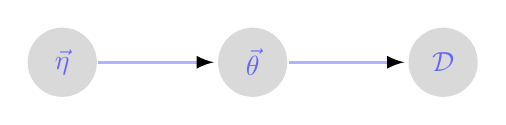
\begin{tikzpicture}[font=\sffamily,node distance=1.5cm,->,>=latex,auto,line width=0.4mm]
	
	\tikzset{node st/.style={state, draw=none,
			fill=gray!30!white,
			text=blue!60!white}}
	
	\node[node st] (I) {$\vec\eta$};
	\node[node st, right=of I] (G) {$\vec\theta$};
	\node[node st, right=of G] (S) {$\mathcal D$};  
	
	
	\draw[every loop,
	auto=right,
	draw=blue!30!white]
	(I) edge[->] node{} (G)
	(G) edge[->] node{} (S);
	
	\end{tikzpicture}
\end{center}

This is an example of a \green{hierarchical Bayesian model}, also called a \green{multi-level model}. 

\myspace
\p \blue{Bayesian Decision Theory} (5.7). Decision problems can be cast as games against nature, where natures selects a quantity $y \in \mathcal Y$ unknown to us, and then generates an observation $\vec x \in \mathcal X$ that we get to see. Our goal is to devise a \green{decision procedure} or \green{policy} $\delta : \mathcal X \mapsto \mathcal A$ for generating an action $a \in \mathcal A$ from observation $\vec x$ that's deemed most compatible with the hidden state $y$. We define ``compatible'' via a loss function $L(y, a)$:
\graybox{
	\delta(\vec x) 
		&= \argmin_{a \in \mathcal A} \rho(a \mid \vec x) \\
	\text{where}\quad
	\rho(a \mid \vec x)
		&= \E[p(y \mid \vec x)]{L(y, a)}
}
In this context, we call $\rho$ the \green{posterior expected loss}, and $\delta(x)$ the \green{Bayes estimator}. Some Bayes estimators for common loss functions are given below.
\begin{compactitem}
	\item \textbf{0-1 loss}: $L(y, a) = \ind\{ y \ne a \}$. Easy to show that $\delta(x) = \argmax_{y \in \mathcal Y} p(y \mid \vec x)$. 
\end{compactitem}



% <>~<>~<>~<>~<>~<>~<>~<>~<>~<>~<>~<>~<>~<>~<>~<>~<>~<>~<>~<>~<>~<>~<>~<>~<>~<>~<>~<>~<>~<>~<>~<>~<>~
\lecture{Machine Learning: A Probabilistic Perspective}{Frequentist Statistics (Ch. 6)}{January 25, 2020}

\vspace{-1.7em}
{\scriptsize Kevin P. Murphy (2012). Bayesian Statistics.\\ \textit{Machine Learning: A Probabilistic Perspective}.\\ }

\bluesec{Sampling Distribution of an Estimator} (6.2). In frequentist statistics, a \green{parameter estimate} $\hat \theta$ is computed by applying an \green{estimator} $\delta$ to some data[set] $\mathcal D$:
\begin{align}
	\hat \theta = \delta(\mathcal D)
\end{align}
\begin{quote}
	\textit{The parameter is viewed as fixed and the data as random, which is the exact opposite of the Bayesian approach.}
\end{quote}
The uncertainty in the parameter estimate can be measured by computing the \green{sampling distribution} of the estimator\marginnote{sampling distribution}. The author's wording contradicts himself here\footnote{Seems to start using ``estimator'' and ``parameter estimate'' interchangeably''}, but basically the sampling distribution, $p(\hat \theta)$, defines the distribution of $\hat \theta$ if we had access to $S \rightarrow \infty$ different datasets $\mathcal{D}^{(s)} = \{x_i^{(s)} \sim p_{\theta^*}\}$ (we often refer to $p_{\theta^*}$ as the true data-generating distribution).  

\bluesec{Frequentist Decision Theory} (6.3). The expected loss or \green{risk} of an estimator $\delta$ is defined as
\graybox{
	R(\theta^*, \delta)
		&\triangleq \E[\widetilde{\mathcal{D}} \sim p_{\theta^*}]{L \lr{ \theta^*, \delta(\widetilde{\mathcal{D}}) } }
}


\bluesec{Desirable Properties of Estimators} (6.4). The \green{bias} of an estimator is defined as
\graybox{
	\text{bias}(\hat{\theta}(\cdot))
		&= \E[\mathcal D \sim p_{\theta^*}]{\hat{\theta}(\mathcal D) - \theta^*}
}

\Needspace{10\baselineskip}
Consider the case where our loss is the quadratic loss $L(\theta^*, \hat{\theta}) = (\theta^* - \hat{\theta})^2$. Then, by definition, the risk is just the MSE. The \green{bias-variance tradeoff} is a useful decomposition of the MSE\footnote{All expectations are taken wrt data-generating distribution, $\mathcal D \sim p(\mathcal D; \theta^*)$.}:
\begin{align}
	\E{(\hat\theta -\theta^*)^2}
		&= \E{\left[ \lr{ \hat\theta - \bar\theta } + \lr{ \bar\theta - \theta^{*}  } \right]^2} \\
		&= \E{(\hat\theta - \bar\theta)^2} + (\bar\theta - \theta^*)^2 \\
		&= \Var{\hat\theta} + \text{Bias}^2(\hat\theta)
\end{align}
where $\bar \theta = \E{\hat\theta}$. 

\begin{example}[Estimating a Gaussian Mean (6.4.4.1)]
	Here I'll derive a lot that the author took as assumed knowledge. We want to estimate the mean of a Gaussian from N data point $\vec x = (x_1, \ldots, x_N)$. We assume the data is sampled from $x_i \sim \Gauss{\theta^*, \sigma^2}$.  \\
	
	\textbf{Derive the MLE of $\theta^*$.} The MLE $\hat\theta$ given data is defined as
	\begin{align}
		\hat\theta 
			&= \argmax_{\theta} \inv{N} \sum_i^N \log \Gauss{x_i; \theta, \sigma^2} \\
			&= \argmax_{\theta} \inv{N} \sum_i^N -\inv{2\sigma^2} (x_i - \theta)^2 \\
		\pderiv{}{\theta} (\cdots)
			&= \inv{N} \sum_i^N \inv{\sigma^2} (x_i - \theta) = 0 \\
		\therefore \hat\theta
			&= \inv{N} \sum_i^N x_i = \bar x
	\end{align}
	
	\textbf{Show that $\E{\hat\theta} = \theta^*$}.
	\begin{align}
		\E[x_1, \ldots, x_N]{\hat\theta}
			&= \E[x_1, \ldots, x_N]{\inv{N}\sum_i x_i}
			= \inv{N}\sum_i \E{x_i}
			= \inv{N} (N \theta^*)
			= \theta^*
	\end{align}
	
	\textbf{Show that $\Var{\hat\theta} = \tfrac{\sigma^2}{N}$}. Since each $x_i$ is sampled independently,
	\begin{align}
		\Var{\hat\theta}
			&= \Var{\inv{N}\sum_i^N x_i} 
			= \inv{N^2}\sum_i \Var{x_i} = \inv{N^2} N \sigma^2 = \frac{\sigma^2}{N}
	\end{align}
	
	Therefore, the bias-variance decomposition for $\hat\theta$ is $MSE = \frac{\sigma^2}{N} + 0^2 = \frac{\sigma^2}{N}$. 
\end{example}







% <>~<>~<>~<>~<>~<>~<>~<>~<>~<>~<>~<>~<>~<>~<>~<>~<>~<>~<>~<>~<>~<>~<>~<>~<>~<>~<>~<>~<>~<>~<>~<>~<>~
\lecture{Machine Learning: A Probabilistic Perspective}{Linear Regression (Ch. 7)}{August 19, 2018}

\vspace{-1.7em}
{\scriptsize Kevin P. Murphy (2012). Linear Regression.\\ \textit{Machine Learning: A Probabilistic Perspective}.\\ }

\p \blue{Model Specification} (7.2). The linear regression model is a model of the form
\begin{align}
	p(y \mid \vec x, \vec\theta)
		&= \mathcal{N}(y \mid \vec{w}^T \vec x, \sigma^2)
\end{align}

\myspace
\p \blue{Maximum Likelihood Estimation} (least squares) (7.3). Most commonly, we'll estimate the parameters by computing the MLE, defined by
\begin{align}
	\hat{\vec{\theta}}
		&\triangleq \argmax_{\theta} \log p(\mathcal D \mid \vec\theta) \\
		&= \argmin_{\theta} \left[ - \log p(\mathcal D \mid \vec\theta) \right] \\
		&= - \inv{2\sigma^2} RSS(\vec w) - \frac{N}{2} \log(2\pi \sigma^2) \\
	RSS(\vec w)
		&\triangleq \sum_{i=1}^{N} (y_i - \vec{w}^T \vec[i]{x})^2
\end{align}
where $RSS(\vec w)$ is the \green{residual sum of squares}. Notice that $\vec\theta := (\vec w, \sigma^2)$, but typically we're focused on estimating $\vec w$\footnote{Since our goal is typically to make future predictions $\hat y(\vec x) = \vec{w}^T\vec{x}$, rather than sampling $y \sim p(y \mid \vec x, \vec\theta)$, we aren't concerned with estimating $\sigma^2$. We assume some variability, and the goal is focused on fitting the data to a straight line.}. 

\myspace
\p \blue{Derivation of the MLE} (7.3.1). We'll now denote the negative log likelihood as $\text{NLL}(\vec w)$ and drop constant terms that are irrelevant for the optimization task. 
\begin{align}
	\text{NLL}(\vec w)
		&= \onehalf || \vec y - \matr X \vec w ||_2^2
		= \onehalf \vec{w}^T (\matr{X}^T \matr{X}) \vec w - \vec{w}^T (\matr{X}^T \vec y) \\
	\text{where}\qquad
	\matr{X}^T\matr{X}
		&= \sum_{i=1}^{N} \vec[i]{x}\vec[i]{x}^T \\
	\matr{X}^T \vec y
		&= \sum_{i=1}^{N} \vec[i]{x} y_i
\end{align}

\Needspace{10\baselineskip}
And the optimal $\vec[OLS]{\hat w}$ be found by taking the gradient, setting to zero, and solving for $\vec w$ as usual:
\graybox{
	\nabla \text{NLL}(\vec w) 
		&= \matr{X}^T \matr X \vec w - \matr{X}^T \vec y \\
	\matr{X}^T \matr X \vec w 
		&= \matr{X}^T \vec y \qquad	\mtgreen{[normal eq.]} \\
	\vec[OLS]{\hat w}
		&= \left(  \matr{X}^T \matr X \right)^{-1} \matr{X}^T \vec y
}

\myspace
\p \blue{Geometric Interpretation} (7.3.2). Use the column-vector representation of $\matr X \in \R^{N \times D}$, where we assume $N > D$\footnote{This means we have more rows than columns, which means our column space cannot span all of $\R^N$.}. Our prediction can then be written
\begin{align}
	\hat{y} &= \matr{X} \vec w = w_1 \vec[1]{\tilde x} + \cdots + w_D \vec[D]{\tilde x}
\end{align}
i.e. a linear combination of the $D$ column vectors $\vec[i]{\tilde x} \in \R^{N}$. Crucially, observe that this means $\hat y \in \text{span}(\{ \vec{\tilde x} \}_i^D)$ no matter what (a hard constraint by definition of our model). So, how do you minimize the residual norm $||\vec y - \vec{\hat y}||$ given that $\vec{\hat y}$ is restricted to a particular subspace? You require $\vec y - \vec{\hat y}$ to be orthogonal to that subspace, of course\footnote{Consider that $\vec y - \hat{\vec y}$ points \textit{from} our prediction (which is in the constraint subspace) $\vec{\hat y}$ \textit{to} the true $\vec y$ that we want to get closest to. Intuitively that means $\vec{\hat y}$ is looking ``straight out'' at $\vec y$, in a direction orthogonal to the subspace that $\vec{\hat y}$ lives in. Formally, we can write $\vec y = (\vec[\parallel]{y}, \vec[\perp]{y})$, where $\vec[\parallel]{y}$ is the component within $\text{Col}(\vec x)$. The best we can do, then, is $\vec{\hat y} := \vec[\parallel]{y} $.}! Formally, this means $\vec[j]{\tilde x}^T ( \vec y - \vec{\hat y}) = 0$, for all $1 \le j \le D$. Equivalently,
\begin{align}
	\matr{X}^T(\vec y - \matr X \vec w) = \vec 0 \quad &\implies \quad \vec{\hat w} = (\matr{X}^T \matr X)^{-1} \matr{X}^T \vec y \\
	\vec{\hat y}
		&= \matr X \vec{\hat w} = \matr{P} \vec{y} \\
	\text{where}\qquad
	\matr P &\triangleq \matr X (\matr{X}^T \matr X)^{-1} \matr{X}^T 
\end{align}
Although this neat, I'm left unsatisfied since there appears to be no intuition of what the column vectors of $\matr X$ really mean on a conceptual level. 

\myspace
\p \blue{Robust Linear Regression} (7.4).\marginnote{Replacing Gaussian with heavy-tailed dists.}[2em] Gaussians sensitive to outliers, since their log-likelihood penalizes deviations quadratically\footnote{In other words, outliers initially get huge loss values, and the distribution shifts toward them to minimize loss (undesirably).}. One way to achieve \green{robustness} to outliers is to instead use a distribution with \green{heavy tails}, such that they still allow for higher likelihoods of outliers, but they don't need to shift the whole distribution around to accommodate for them. One popular choice is the \green{Laplace distribution},
\begin{align}
	p(y \mid \vec x , \vec w, b)
		&= \text{Lap}(y \mid \vec{w}^T \vec x, b)
		\triangleq \inv{2b} \exp\left\{ - \inv{b} | y - \vec{w}^T\vec x  | \right\} \\
	NLL(\vec w)
		&= \sum_i | y_i - \vec{w}^T \vec[i]{x} |
\end{align}
Goal: convert $NLL$ to a form easier to optimize (linear). Let $r_i \triangleq y_i - \vec{w}^T \vec[i]{x}$ be the i'th residual. The following steps show how we can convert this into a \green{linear program}:
\begin{align}
	r_i
		&\triangleq r_i^+ - r_i^- \qquad (r_i^+ \ge 0)(r_i^- \ge 0)     \\
	\min_{\vec w, \vec{r}^+, \vec{r}^-} \sum_i (r_i^+ + r_i^-)
	\qquad&\text{s.t.}\qquad \vec{w}^T\vec[i]{x} + r_i^+ - r_i^- = y_i \\
	\min_{\vec\theta} \vec{f}^T \vec{\theta}
	\qquad&\text{s.t.}\qquad \matr A \vec{\theta} \le \vec b, ~ \matr[eq]{A}\vec{\theta} = \vec[eq]{b}, ~ \vec 1 \le \vec\theta \le \vec u
\end{align}
where the last equation is the \green{standard form} of a LP. 

\myspace 
\p \blue{Ridge Regression} (7.5).\marginnote{Doing MAP instead of MLE}[2em] We know that MLE can overfit by essentially memorizing the data. If, for example, we model 21 points with a degree-14 polynomial\footnote{To review polynomials, search ``Lagrange interpolation'' in your CS 70 notes.}, we get many large positive and negative numbers for our learned coefficients, which allow the curve to wiggle in just the right way to almost perfectly interpolate the data -- \textbf{this is why we often regularize weights to have low absolute value}. This encourages smoother/less-wiggly curves. One way to do this is by using a zero-mean Gaussian prior on our weights:
\begin{align}
	p(\vec w)
		&= \prod_j \mathcal{N}(w_j \mid 0, \tau^2)
\end{align}
This makes our MAP estimation problem and solution take the form\marginnote{Note that $w_0$ is NOT regularized.}[2em]
\graybox{
	J(\vec w) 
		&= \inv{N} \sum_i^N \left(  y_i - \vec{w}^T \vec[i]{x} - w_0  \right) + \lambda ||\vec w||_2^2 \\
	\vec[ridge]{\hat w}
		&= ( \matr{X}^T \matr X + \lambda \matr[D]{I}  )^{-1} \matr{X}^T \vec y
}




% <>~<>~<>~<>~<>~<>~<>~<>~<>~<>~<>~<>~<>~<>~<>~<>~<>~<>~<>~<>~<>~<>~<>~<>~<>~<>~<>~<>~<>~<>~<>~<>~<>~
\lecture{Machine Learning: A Probabilistic Perspective}{Generalized Linear Models and the Exponential Family (Ch. 9)}{August 11, 2018}

\vspace{-1.7em}
{\scriptsize Kevin P. Murphy (2012). Generalized Linear Models and the Exponential Family.\\ \textit{Machine Learning: A Probabilistic Perspective}.\\ }

\p \blue{The Exponential Family} (9.2). Why is the exponential family important?
\begin{compactitem}
	\item It's the only family with \textbf{finite-sized sufficient statistics}\footnote{Given certain regularity conditions.}. 
	\item It's the only family for which \textbf{conjugate priors exist}.
	\item It makes the \textbf{least set of assumptions} subject to some user-chosen constraints.
	\item It's at the core of GLMs and variational inference. 
\end{compactitem}
\begin{definition}
	A pdf or pmf $p(\vec x \mid \vec\theta)$, for $\vec x \in \mathcal{X}^m$ and $\vec\theta \in \Theta \subseteq \R^d$, is said to be in the \green{exponential family} if it's of the form\marginnote{$h(\vec x)$ is a scaling constant, often 1.}[2em]
	\graybox{
		p(\vec x \mid \mgreen{\vec\theta})
			&= \inv{Z(\mgreen{\vec\theta})} h(\vec x) \exp\{ \mgreen{\vec\theta}^T \mpurple{\vec{\phi}(\vec x)} \}
			= h(\vec x) \exp\left\{ \mgreen{\vec\theta}^T \mpurple{\vec{\phi}(\vec x)} - A(\mgreen{\vec\theta})   \right\}	\\
		Z(\mgreen{\vec\theta})
			&= \int_{\mathcal{X}^m} h(\vec x) \exp\{\mgreen{\vec\theta}^T\mpurple{\vec{\phi}(\vec x)} \} \\
		A(\mgreen{\vec\theta})
			&= \log Z(\mgreen{\vec\theta}) 
	}
where $ \mgreen{\vec\theta}$ are the \green{natural (canonical) parameters}\footnote{We often generalize this with $\vec{\eta}(\vec\theta)$, which maps whatever params $\vec\theta$ we've chosen to the canonical params $\vec{\eta}(\vec\theta)$.}, and $\mpurple{\vec{\phi}(\vec x)}$ are the \purple{sufficient statistics}. 
\end{definition}
Below are some (quick/condensed) examples showing the first couple steps in rewriting familiar distributions in exponential family form:
\begin{align}
	\mtgreen{[Bernoulli]}&\quad \text{Ber}(x \mid \mu)
		= \mu^x (1 - \mu)^{1- x} = \exp\{  x \log \mu + (1 - x) \log(1- \mu)   \}  \\
	\mtgreen{[Multinoulli]}&\quad \text{Cat}(x \mid \vec\mu)
		= \prod_k^K \mu_k^{x_k} = \exp\left\{  \sum_k^{K-1} x_k \log\left(\mu_k/\mu_K \right) + \log\mu_K  \right\} 
\end{align}

\myspace
\p \blue{Log Partition Function} (9.2.3). The derivatives of the log partition, $A(\vec\theta)$, can be used to generate \green{cumulants}\footnote{The first and second cumulants are mean and variance.} for the sufficient statistics, $\vec{\phi}(\vec x)$. 
\begin{align}
	\pderiv{A(\vec\theta)}{\vec\theta} &= \E{\vec{\phi}(\vec x)} \\
	\nabla^2 A(\vec\theta) &= \text{cov}\left[ \vec{\phi}(\vec x) \right]
\end{align}


\myspace
\p \blue{MLE for the Exponential Family} (9.2.4). The likelihood takes the form\marginnote{It appears that we are denoting $1/Z$ with $g$ now.}[3em]
\begin{align}
	p(\mathcal D \mid \vec\theta)
		&= \left[ \prod_i^N h(\vec{x}^{(i)}) \right] g(\vec\theta)^N \exp\left\{ \vec{\eta}(\vec\theta)^T \vec{\phi}(\mathcal D) \right\} \\
	\vec{\phi}(\mathcal D) 
		&=  \sum_i^N \vec{\phi}(\vec{x}^{(i)}) 
		= \begin{bmatrix} \sum_i \phi_1 & \cdots & \sum_i \phi_K  \end{bmatrix}
\end{align}
where I've denoted $\sum_{i=1}^N \phi_k(\vec{x}^{(i)})$ as simply $\sum_i \phi_k$. The \green{Pitman-Koopman-Darmois theorem} states, given certain regularity conditions/constraints\footnote{The wording is weird here. We mean ``out of all families/distributions that \textit{already} satisfy certain constraints that must be met, the exponential family is the only...''. For example, the uniform distribution has finite statistics and is not in the exponential family, but it does not meet the constraint that its support must be independent of the parameters, so it's outside the scope of the theorem.}, that the exponential family is the only family with \textit{finite sufficient statistics} (dimensionality independent of the size of the data set). For example, in the above formula, we have $K + 1$ sufficient statistics ($+1$ since we need to know the value of $N$). \\

\p Consider a canonical\footnote{Defined as those which satisfy $\vec{\eta}(\vec\theta) = \vec\theta$.} exponential family which also sets $h(\cdot) = 1$. The log-likelihood is
\begin{align}
	p(\mathcal D \mid \vec\theta)
		&= \vec\theta^T \vec{\phi}(\mathcal D) - N A (\vec\theta)
\end{align}
Since $-A(\vec\theta)$ is concave\footnote{We know $-A$ is concave because $A$ is convex. We know $A$ is convex because $\nabla^2 A$ is positive definite. Remember that any twice-differentiable multivariate function $f$ is convex IFF its Hessian is pd for all $\vec\theta$. See sec 7.3.3 and 9.2.3 for more.} and the other term is linear in $\vec\theta$, the log-likelihood is concave and thus has a global maximum.

\myspace
\p \blue{Maximum Entropy Derivation of the Exponential Family} (9.2.6). Suppose we don't know which distribution $p$ to use, but we do know the expected values of certain features or functions:
\begin{align}
	F_k \triangleq \E[\vec x \sim p(\rvec x)]{f_k(\vec x)} = \sum_{\vec x} f_k(\vec x) p(\vec x)
\end{align}
The principle of \green{maximum entropy} or \green{maxent} says we should pick the distribution with maximum entropy, subject to the constraints that the moments of the distribution match the empirical moments of the specified functions $f_k(\vec x)$. Treating $p$ as a fixed length vector (i.e. assuming $\vec x$ is discrete), we can take the derivative of our Lagrangian (entropy in units of nats with constraints) w.r.t. each ``element'' $p_x = p(\vec x)$ to find the optimal distribution.
\begin{align}
	J(p, \vec\lambda)
		&= H(p) + \lambda_0 \left( 1 - \sum_{\vec x} p(\vec x) \right) + \sum_k \lambda_k \left(F_k - \sum_{\vec x} p(\vec x) f_k(\vec x) \right) \\
	\pderiv{J}{p(\vec x)}
		&= -1 - \log p(\vec x) - \lambda_0 - \sum_k \lambda_k f_k(\vec x)
\end{align}
Setting this derivative to zero yields
\begin{align}
	p(\vec x) 
		&= \inv{Z} \exp\left\{ -\sum_k \lambda_k f_k(\vec x)  \right\}
\end{align}
Thus the maxent distribution $p(\vec x)$ has the form of the exponential family, a.k.a. the \green{Gibbs distribution}. 











% <>~<>~<>~<>~<>~<>~<>~<>~<>~<>~<>~<>~<>~<>~<>~<>~<>~<>~<>~<>~<>~<>~<>~<>~<>~<>~<>~<>~<>~<>~<>~<>~<>~
\lecture{Machine Learning: A Probabilistic Perspective}{Mixture Models and the EM Algorithm (Ch. 11)}{August 26, 2018}

\vspace{-1.7em}
{\scriptsize Kevin P. Murphy (2012). Mixture Models and the EM Algorithm.\\ \textit{Machine Learning: A Probabilistic Perspective}.\\ }

\p \blue{Latent Variable Models} (LVMs) (11.1). In this chapter, we explore directed GMs that have hidden/latent variables. Advantages of LVMs:
\begin{compactenum}
	\item Often have fewer params.
	\item Hidden vars can serve as a bottleneck (representation learning).
\end{compactenum}

\myspace
\p \blue{Mixture Models} (11.2). The simplest form of LVM is where the hidden variables $z_i \in \{1, \ldots, K\}$ represent a discrete latent state. We use discrete prior $p(z_i) = \text{Cat}(\vec\pi) = \pi_i$, and likelihood $p(\vec[i]{x} \mid z{=}k) = p_k(\vec[i]{x})$. A \green{mixture model} is defined by\marginnote{We call $p_k$ the $k$th \textbf{base distribution}.}[2em]
\graybox{
	p(\vec[i]{x} \mid \vec\theta)
		&= \sum_{k=1}^{K} \pi_k p_k(\vec[i]{x} \mid \vec\theta)	
}
Some popular mixture models:
\begin{compactitem}
	\item \green{Mixture of Gaussians} (11.2.1). Each $p_k = \mathcal{N}(\vec[k]{\mu}, \matr[k]{\Sigma})$. Given large enough $K$, \textit{a GMM can approximate any density defined on $\R^D$.}
	
	\item \green{Mixture of Multinoullis} (11.2.2). Let $\vec x \in \{0, 1\}^D$. Each $p_k(\vec x) = \prod_j^D \text{Ber}(x_j \mid \mu_{jk})$. Below, I derive the expectation and covariance of $\vec x$ in this case\footnote{Shown in excruciating detail because I was unable to work through this in my head alone.}. 
	\begin{align}
		\E{\rvec x}
			&= \sum_{\vec x} \vec{x} p(\vec x) \\
			&= \sum_{\vec x} \vec{x} \sum_k^K \pi_k p_k(\vec x) \\
			&= \sum_{\vec x} \vec{x} \sum_k^K \pi_k \prod_{j}^{D} \text{Ber}(x_j\mid \mu_{jk}) \\
			&= \sum_k^{D} \pi_k \sum_{x_1} \cdots \sum_{x_D} \vec x \prod_j^D \text{Ber}(x_j\mid \mu_{jk}) \\
			&= \sum_k^{D} \pi_k \sum_{x_1} \text{Ber}(x_1 \mid \mu_{1k}) \cdots \sum_{x_D} \text{Ber}(x_D \mid \mu_{Dk}) \vec x \\
			&= \sum_k^{D} \pi_k \vec[k]{\mu} 
	\end{align}
	Next we want to find $\text{cov}(\rvec x) = \E{\rvec{x}\rvec{x}^T} - \E{\rvec x}\E{\rvec{x}}^T$. I think the insight that makes finding the first term easiest is realizing that you only need to find the two cases, $\E{x_i^2}$ and $\E{x_i x_{j\ne i}}$, where in this case
	\begin{align}
		\E{x_i^2} &= \sum_k \pi_k \mu_{ik} \\
		\E{x_i x_{j \ne i}} &= \sum_k \pi_k \mu_{ik} \mu_{jk} \\
		\therefore \E{\rvec x \rvec{x}^T}
			&= \sum_k \pi_k \left( \matr[k]{\Sigma} + \vec[k]{\mu} \vec[k]{\mu}^T  \right)
	\end{align}
	where $\Sigma_k = \text{diag}(\mu_{jk}(1- \mu_{jk}))$ is the covariance of $\vec x$ under $p_k$. The fact that the mixture covariance matrix is now non-diagonal confirms that the mixture can capture correlations between variables $x_i, x_{j\ne i}$, unlike a single product-of-Bernoullis model.
	
\end{compactitem}

\myspace
\p \blue{The EM Algorithm} (11.4). In LVMs, it's usually intractable to compute the MLE since we have to marginalize over hidden variables while satisfying constraints like positive definite covariance matrices, etc. The EM algorithm gets around these issues via a two-step process. The first step involves taking an expectation, where the expectation is over $\vec z \sim p(\vec z \mid \vec x, \theta^{t-1})$ for each individual observed $\vec x$, where we use the current parameter estimates when sampling $\vec z$ in the expectation. \textbf{This gives us an auxiliary likelihood that's a function of $\vec\theta$} which will serve as a stand-in (in the 2nd step) for what we typically use as the likelihood in MLE. The second step is then just finding the optimal $\vec{\theta}^t$ over the auxiliary likelihood function from the first step. This iterates until convergence or some stopping condition.

\begin{algorithm}[Procedure: EM Algorithm]

First, let's define our auxiliary function $Q$ as
	\begin{align}
		Q(\vec\theta \mid \vec{\theta}^{t-1})
			&= \E[p(\vec z \mid \vec x, \vec{\theta}^{t-1})]{\ell_c(\vec\theta) \mid \mathcal{D}} \\
		\text{where}\quad
		\ell_c(\vec\theta)
			&= \sum_{i=1}^{N} \log p(\vec{x}^{(i)}, \vec{z}^{(i)} \mid \vec\theta)
	\end{align}
	where, again, the ``expectation'' serves the purpose of determining the expected value of $\vec{z}^{(i)}$ for each observed $\vec{x}^{(i)}$. It's somewhat of a misnomer to denote the expectation like this, since each $\vec{z}^{(i)}$ is innately tied with its corresponding observation $\vec{x}^{(i)}$.
	
	\begin{compactenum}
		\item \textbf{E-Step}: Evaluate $Q(\vec\theta \mid \vec{\theta}^{t-1})$ using (obviously) the previous parameters $\vec{\theta}^{t-1}$. This yields a function of $\vec\theta$. This gives us the expected log-likelihood function of $\vec\theta$ for the observed data $\mathcal D$. 
		
		\item \textbf{M-Step}: Optimize $Q$ w.r.t $\vec\theta$ to get $\vec{\theta}^t$:
		\begin{align}
			\vec{\theta}^t 
				&= \argmax_{\vec\theta} Q(\vec\theta \mid \vec{\theta}^{t-1})
		\end{align}
	\end{compactenum}

\end{algorithm}








% <>~<>~<>~<>~<>~<>~<>~<>~<>~<>~<>~<>~<>~<>~<>~<>~<>~<>~<>~<>~<>~<>~<>~<>~<>~<>~<>~<>~<>~<>~<>~<>~<>~
\lecture{Machine Learning: A Probabilistic Perspective}{Latent Linear Models (Ch. 12)}{September 14, 2018}

\vspace{-1.7em}
{\scriptsize Kevin P. Murphy (2012). Latent Linear Models.\\ \textit{Machine Learning: A Probabilistic Perspective}.\\ }

\p \blue{Factor Analysis} (12.1). Whereas mixture models define $p(z) = \text{Cat}(\vec\pi)$ for a single hidden variable $z \in \{1, \ldots, K\}$, \green{factor analysis} begins by instead using a \textit{vector} of \textit{real-valued} latent variables, $\vec z \in \R^{L}$. The simplest prior is $\vec z \sim \mathcal{N}(\vec[0]{\mu}, \matr[0]{\Sigma})$. If $\vec x \in \R^D$, we can define
\begin{align}
	p(\vec[i]{x}\mid \vec[i]{z}, \vec\theta)
		&= \mathcal{N}(\matr W \vec[i]{z} + \vec\mu, \matr\Psi)
\end{align}
where
\begin{compactitem}
	\item $\matr W \in \R^{D \times L}$: \green{factor loading matrix}.
	
	\item $\matr\Psi \in \R^{D \times D}$ is a \underline{diagonal} covariance matrix, since we want to ``force'' $\vec{z}$ to explain the correlation\footnote{It's easier to think of this graphically. Our model asserts that $\vec[i]{x} \perp \vec[j\ne i]{x} \mid \vec{z}$. Independence implies zero correlation, and we cement this by constraining $\matr\Psi$ to be diagonal. See your related note on LFMs, chapter 13 of the DL book.}. If $\matr\Psi  = \sigma^2 \matr I$, we get \green{probabilistic PCA}. 
\end{compactitem}
Summaries of key points regarding FA:
\begin{compactitem}
	\item \textbf{Low-rank parameterization of MVN}. FA can be thought of as specifying $p(\vec x)$ using a small number of parameters. [math] yields that
	$$
	\text{cov}(\vec x) = \matr W \matr{W}^T + \matr\Psi
	$$
	which has $\mathcal{O}(LD)$ params (remember $\matr\Psi$ is diagonal) instead of the usual $\mathcal{O}(D^2)$. 
	
	\item \textbf{Unidentifiability}: The params of an FA model are unidentifiable. 
\end{compactitem}

\myspace
\p \blue{Classical PCA} (12.2.1). Goal: find an orthogonal set of $L$ linear basis vectors $\vec[j]{w} \in \R^D$, and the scores $\vec[i]{z} \in \R^L$, such that we minimize the average \green{reconstruction error}:
\begin{align}
	J(\matr W, \matr Z)
		&= \inv{N} \sum_{i=1}^{N} || \vec[i]{x} - \vec[i]{\hat x} ||^2, 
		\quad\text{where}\quad
		\vec[i]{\hat x} := \matr W \vec[i]{z} \\
		&= || \matr X - \matr W \matr{Z}^T ||_F^2
\end{align}
where $\matr W \in \R^{D \times L}$ is orthonormal. \textbf{Solution}: assign each column $\matr[:,\ell]{W}$ to the eigenvector with $\ell$'th largest eigenvalue of $\matr{\hat \Sigma} = \inv{N} \sum_i^N \vec[i]{x}\vec[i]{x}^T$, assuming $\E{\vec x} = \vec{0}$. Then we compute $\vec[i]{\hat z} := \matr{W}^T \vec[i]{x}$. 

\begin{example}[Proof: PCA]
	\textbf{Case: L=1}. Goal: Find the best 1-d solution, $\vec{w} \in \R^D$, $z_i \in \R$, $\vec z \in \R^N$. Remember that $||\vec w||_2 = 1$. 
	\begin{align}
		J(\vec w, \vec{z})
			&= \inv{N} \sum_i^N || \vec[i]{x} - z_i \vec{w} ||^2 
			= \inv{N} \left[   \vec[i]{x}^T \vec[i]{x} - 2 z_i \vec{w}^T \vec[i]{x} + z_i^2  \right] \\
		\pderiv{J}{z_i}
			&= 0 \quad\rightarrow\quad z_i = \vec{w}^T\vec[i]{x} \\
		J(\vec w)
			&= \inv{N}\sum_i^N \left[ \vec[i]{x}^T\vec[i]{x} - z_i^2 \right]
			= \text{const} - \inv{N} \sum_i^N z_i^2 \\
		\therefore
		\argmin_{\vec w} J(\vec w) 
			&= \argmax_{\vec w} \text{Var}\left[  \vec{\tilde z} \right]
	\end{align}
	This shows why PCA finds directions of maximal variance -- aka the \purple{analysis view} of PCA. Before finding the optimal $\vec w$, don't forget the Lagrange multipliers for constraining unit norm,
	\begin{align}
		\tilde{J}(\vec w)
			&= \vec{w}^T \matr{\hat \Sigma} \vec{w} + \lambda (\vec{w}^T \vec w - 1)
	\end{align}
\end{example}

\myspace
\p \blue{Singular Value Decomposition} (SVD) (12.2.3). Any real $N \times D$ matrix $\matr X$ can be decomposed as
\begin{align}
	\matr X
		&= \underbrace{\matr U}_{N \times N} \underbrace{\matr S}_{N \times D} \underbrace{\matr{V}^T}_{D \times D}
\end{align}
where the columns of $\matr U$ are the left singular vectors, and the columns of $\matr V$ are the right singular vectors. \textbf{Economy-sized SVD} will shrink $\matr U$ to be $N \times D$ and $\matr S$ to be $D \times D$ (we're assuming N > D). 




% <>~<>~<>~<>~<>~<>~<>~<>~<>~<>~<>~<>~<>~<>~<>~<>~<>~<>~<>~<>~<>~<>~<>~<>~<>~<>~<>~<>~<>~<>~<>~<>~<>~
\lecture{Machine Learning: A Probabilistic Perspective}{Markov and Hidden Markov Models (Ch. 17)}{August 11, 2018}

\vspace{-1.7em}
{\scriptsize Kevin P. Murphy (2012). Markov and Hidden Markov Models.\\ \textit{Machine Learning: A Probabilistic Perspective}.\\ }

\p \blue{Hidden Markov Models} (17.3). HMMs model a joint distribution over a sequence of $T$ observations $\slice[T]{x}$ and hidden states $\slice[T]{z}$,
\begin{align}
	p(\slice[T]{z}, \slice[T]{x})
		&= p(\slice[T]{z}) p(\slice[T]{x} \mid \slice[T]{z})
		= \left[ p(z_1) \prod_{t=2}^{T} p(z_t \mid z_{t-1})  \right]
			\left[ \prod_{t=1}^T p(\vec[t]{x} \mid z_t) \right]
\end{align}
where each hidden state is discrete: $z_t \in \{1, \ldots, K \}$, while each observation $\vec[t]{x}$ can be discrete or continuous.

\myspace
\p \blue{The Forwards Algorithm} (17.4.2). Goal: compute the filtered\footnote{They're called ``filtered'' because they use all observations $\slice[t]{x}$ instead of just $\vec[t]{x}$, which reduces/filters out the noise more.} marginals $p(z_t \mid \slice[t]{x})$.
\begin{compactenum}
	\item \textbf{Prediction step}. Compute the \textit{one-step-ahead predictive density} $p(z_t \mid \slice[t-1]{x})$,
	\begin{align}
		p(z_t {=} j \mid \slice[t-1]{x})
			&= \sum_i p(z_t = j, z_{t-1} = i \mid \slice[t-1]{x}) 
	\end{align}
	which will serve as our prior for time $t$ (since it does not take into account observed data at time t). 
	
	\item \textbf{Update step}. We ``update'' our beliefs by observing $\vec[t]{x}$,
	\begin{align}
		\alpha_t(j)
			&\triangleq p(z_t {=} j \mid \slice[t]{x}) \\
			&= \frac{  p(z_t {=} j, \vec[t]{x}, \slice[t-1]{x}) }{  p(\slice[t]{x}) } \\
			&= \frac{ \cancel{ p(\slice[t-1]{x}) } p(z_t{=}j \mid \slice[t-1]{x}) p(\vec[t]{x} \mid z_t {=} j, \cancel{ \slice[t-1]{x}  }) }{
				\cancel{  p(\slice[t-1]{x}) } p(\vec[t]{x} \mid \slice[t-1]{x}) } \\
			&= \inv{Z_t} p(z_t {=} j \mid \slice[t-1]{x}) p(\vec[t]{x} \mid z_t {=} j)
	\end{align}
\end{compactenum}
Notice that we can also use the values of $Z_t$ to compute the log probability of the evidence:
\begin{align}
	\log p(\slice[T]{x} \mid \vec\theta)
		&= \sum_{t=1}^{T} \log p(\vec[t]{x} \mid \slice[t-1]{x}) 
		= \sum_{t=1}^T \log Z_t
\end{align}

\begin{algorithm}[Forwards Algorithm (Algorithm 17.1)]
	We are given transition matrix $T_{i,j} = p(z_t = j \mid z_{t-1} = i)$, evidence vectors $\psi_t(j) = p(\vec[t]{x} \mid z_t{=}j)$, and initial state distribution $\pi(j) = p(z_1 = j)$. 
	
	\begin{compactenum}
		\item First, compute the initial $[\alpha_1, Z_1] = \text{normalize}(\psi_1 \odot \pi)$. 
		
		\item For time $2 \le t \le T$, compute $[\alpha_t, Z_t] = \text{normalize}(\psi_t \odot \matr{T}^T \vec[t-1]{\alpha})$. 
		
		\item Return $\slice[T]{\alpha}$ and $\log p(\slice[T]{x}) = \sum_t \log Z_t$. 
	\end{compactenum} 
\end{algorithm}

\myspace
\p \blue{The Forwards-Backwards Algorithm} (17.4.3). Goal: compute the smoothed marginals, $p(z_t = j \mid \slice[T]{x})$. 
\begin{align}
	\gamma_t(j)
		&\triangleq p(z_t = j \mid \slice[T]{x})   \\
		&\propto p(z_t = j \mid \slice[t]{x}) p(\slice[T][t+1]{x} \mid z_t = j) \\
		&= \alpha_t(j) \beta_t(j) \\
	\text{where}\quad
	\beta_t(j)
		&\triangleq p(\slice[T][t+1]{x} \mid z_t {=} j)  \\
		&= p(\vec[t+1]{x}, \slice[T][t+2]{x} \mid z_t{=}j ) \\
		&= \sum_{i} p(z_{t+1}{=}i, \vec[t+1]{x}, \slice[T][t+2]{x} \mid z_t{=}j ) \\
		&= \sum_i p(z_{t+1}{=}i, \vec[t+1]{x} \mid z_t{=}j) p(\slice[T][t+2]{x} \mid \cancel{z_t{=}j}, z_{t+1}{=}i, \cancel{\vec[t+1]{x}} ) \\
		&= \sum_i p(z_{t+1}{=}i \mid z_t{=}j) p(\vec[t+1]{x} \mid z_{t+1}{=}i) p(\slice[T][t+2]{x} \mid z_{t+1}{=}i) \\
		&=  \sum_i p(z_{t+1}{=}i \mid z_t{=}j) p(\vec[t+1]{x} \mid z_{t+1}{=}i) \beta_{t+1}(i)
\end{align}
Using the same notation as Algorithm 17.1 above, the matrix-vector form for $\beta$ is
\begin{align}
	\vec[t]{\beta} &= \matr{T} \left( \vec[t]{\psi} \odot \vec[t+1]{\beta}  \right)
\end{align}
with base case $\vec[T]{\beta} = \vec{1}$. 

\myspace
\p \blue{The Viterbi Algorithm} (17.4.4). Denote the [probability for] the most probable path leading to $z_t{=}j$ as\marginnote{It is common to work in the log-domain when computing $\delta$.}[2em]
\begin{align}
	\delta_t(j) 
		&\triangleq \max_{\slice[t-1]{z}} p(\slice[t-1]{z}, z_t{=}j \mid \slice[t]{x}) \\
		&= \max_i \delta_{t-1}(i) \cdot T_{i,j} \cdot  \psi_t(j)
\end{align}
with initialization of $\delta_1(j) = \pi_j \psi_1(j)$. We compute this until termination at $z_{T}^* = \argmax_i \delta_T(i)$. Note the $\argmax$ here instead of a $\max$ -- we keep track of both for all time steps. We do this so we can perform \green{traceback} to get the full most probable state sequence, starting at $T$ and ending at $t=1$:
\begin{align}
	z_t^* &= a_{t+1}(z_{t+1}^*)
\end{align}
where $a_t(j)$, the most probable state at time $t-1$ leading to state $j$ at time $t$, is the same formula as $\delta_t(j)$ but with an $\argmax$. 






























% <>~<>~<>~<>~<>~<>~<>~<>~<>~<>~<>~<>~<>~<>~<>~<>~<>~<>~<>~<>~<>~<>~<>~<>~<>~<>~<>~<>~<>~<>~<>~<>~<>~
\lecture{Machine Learning: A Probabilistic Perspective}{Undirected Graphical Models (Ch. 19)}{August 11, 2018}

\vspace{-1.7em}
{\scriptsize Kevin P. Murphy (2012). Undirected Graphical Models.\\ \textit{Machine Learning: A Probabilistic Perspective}.\\ }

\p \blue{Learning} (19.5). Consider a MRF in log-linear form over $C$ cliques and its log-likelihood (scaled by 1/N):
\begin{align}
	p(\vec y \mid \vec\theta)	
		&= \inv{Z(\vec\theta)} \exp\left\{ \sum_c \vec[c]{\theta}^T \vec[c]{\phi}(\vec y)  \right\} \\
	\ell(\vec\theta)
		&= \inv{N} \sum_i \left[ \sum_c  \vec[c]{\theta}^T \vec[c]{\phi}(\vec[i]{y}) - \log Z(\vec\theta)    \right]
\end{align}
We know from chapter 9 that this log-likelihood is concave in $\vec\theta$, and that $\pderiv{}{\vec[c]{\theta}} \log Z = \E{\phi_c}$. So the gradient of the LL is
\begin{align}
	\pderiv{\ell}{\vec[c]{\theta}} 
		&= \left[ \inv{N} \sum_i \vec[c]{\phi}(\vec[i]{y}) \right] - \E[p(\vec y \mid \vec\theta)]{\vec[c]{\phi}(\vec y)}
\end{align}
Note that the first (``clamped'') term only needs to be computed once for any $\vec[i]{y}$, it is completely independent of any parameters. It's just evaluating feature functions, which e.g. for CRFs are often all indicator functions.

\myspace
\p \blue{CRF Training} (19.6.3). For [linear-chain] CRFs, the equations change slightly (but importantly).
\begin{align}
	\ell(\vec w)
		&\triangleq \inv{N} \sum_i \left[ \sum_c \vec[c]{w}^T \vec[c]{\phi}(\vec[i]{y}, \vec[i]{x}) - \log Z(\vec w, \vec[i]{x}) \right] \\
	\pderiv{\ell}{\vec[c]{w}}
		&= \inv{N} \sum_i \left[
			\vec[c]{\phi}(\vec[i]{y}, \vec[i]{x}) 
		- \E[ p( \vec{y} \mid  \bm{x}_i ) ]{ \vec[c]{\phi}(\vec[i]{y}, \vec[i]{x}) }		
		\right]
\end{align}
It's important to recognize that the gradient of the log partition function now must be computed for \textit{each} instance $\vec[i]{x}$. 




% ==================================================================================
% ==================================================================================
% ==================================================================================
% Convex Optimization
% ==================================================================================
% ==================================================================================
% ==================================================================================
\mysection{Convex Optimization}\label{Convex Optimization}

\newcommand{\relint}{\rvec{relint}}
\newcommand{\aff}{\rvec{aff}}
\newcommand{\conv}{\rvec{conv}}

% ======================================================================================
\lecture{Convex Optimization}{Convex Sets (Ch. 2)}{August 19, 2018}
% ======================================================================================
\vspace{-1.7em}
{\scriptsize Boyd and Vandenberghe (2004). Convex Sets.\\ \textit{Convex Optimization}.\\ }


\begin{definition}[-1em][Lines and line segments]
	Viewed as a function of $\theta \in \R$, we can express the equation for a \green{line} in $\R^n$ in the following two ways:
	\begin{align}
		y &= \theta x_1 + (1 - \theta) x_2 \\
		y &= x_2 + \theta (x_1 - x_2)
	\end{align}
	for some $x_1, x_2{\ne}x_1 \in \R^n$. If we restrict $\theta \in [0, 1]$, we have a \green{line segment}. 
\end{definition}

\begin{definition}[-1em][Affine sets]
	A set $C \subseteq \R^n$ is \green{affine} if the \textit{line} (not just segment) through any two distinct points in $C$ also lies in $C$. More generally, this implies that for any set of points $\{x_1, \ldots, x_k\}$, with each $x_i \in C$, all \green{affine combinations},
	\begin{align}
		\sum_{i=1}^{k} \theta_i x_i, \quad\text{where}\quad \sum_i \theta_i = 1
	\end{align}
	are in $C$, too. Related terminology:
	\begin{compactitem}
		\item \green{affine hull} of any set $C \subseteq \R^n$, denoted $\rvec{aff}C$, is the set of all affine combinations of points in $C$. 
		
		\item \green{affine dimension} of a set $C$ is the dimension of its affine hull. 
		
		\item \green{relative interior} of a set $C$, denoted $\rvec{relint}C$, is its interior\footnote{
			The \purple{interior of a set} $C \subseteq \R^n$, denoted $\rvec{int}C$, is the set of all points interior to $C$. A point $x \in C$ is interior to $C$ if $\exists \epsilon > 0$ for which \textit{all points} in the set
			$$
			\{ y \in R^n \mid ||y - x||_2 \le \epsilon  \}
			$$
			are also in $C$.
		}
		relative to $\rvec{aff}C$,
		\begin{align}
			\rvec{relint}C
				&\triangleq \{  x \in C \mid B(x, r) \cap \aff C \subseteq C  ~\text{for some}~ r > 0  \}
		\end{align}
	\end{compactitem}
\end{definition}
There's a lot of neat things to say here, but I only have space to state the results:
\begin{compactitem}
	\item If $C$ is an affine set and $x_0 \in C$, then
	\begin{align}
		V = C - x_0 \triangleq \{ x - x_0 \mid x \in C  \}
	\end{align}
	is a \textit{subspace}, i.e. closed under sums and scalar multiplication. 
	
	\item The solution set of a system of linear equations, $C = \{ x \mid Ax=b  \}$, is an affine set. The subspace associated with $C$ is the \textit{nullspace} of $A$. 
\end{compactitem}


\begin{definition}[-1em][Convex sets]
	A set $C$ is \green{convex} if it contains all \green{convex combinations},
	\begin{align}
		\sum_{i=1}^{k} \theta_i x_i, \quad\text{where}\quad \sum_i \theta_i = 1, ~\text{and}~ \theta_i \ge 0
	\end{align}
	Related terminology:
	\begin{compactitem}
		\item \green{convex hull} a set $C$, denoted $\conv C$, is the set of all convex combinations of points in $C$. 
	\end{compactitem}
\end{definition}


\begin{definition}[-1em][Cones]
	A set $C$ is called a \green{cone} if $(\forall x \in C)(\theta \ge 0)$ we have $\theta x \in C$. A set $C$ is called a \green{convex cone} if it contains all \green{conic combinations},
	\begin{align}
		\sum_{i=1}^{k} \theta_i x_i, \quad\text{where}\quad \theta_i \ge 0
	\end{align}
	of points in $C$. Related terminology:
	\begin{compactitem}
		\item \green{conic hull} of a set $C$ is the set of all conic combinations of points in $C$.
	\end{compactitem}
\end{definition}





















% ==================================================================================
% ==================================================================================
% ==================================================================================
% BDA
% ==================================================================================
% ==================================================================================
% ==================================================================================
\mysection{Bayesian Data Analysis}\label{Bayesian Data Analysis}


% ======================================================================================
\lecture{Bayesian Data Analysis}{Probability and Inference (Ch. 1)}{November 22, 2017}
% ======================================================================================

\p The process of Bayesian Data Analysis can be divided into the following 3 steps:
\begin{compactenum}
	\item Setting up a \textit{full probability model}.
	\item Conditioning on observed data. Calculating the \textit{posterior distribution} over unobserved quantities, given observed data.
	\item Evaluating the fit of the model and implications of the posterior. 
\end{compactenum}
\textbf{Notation}: In general, we let $\theta$ denote unobservable vector quantities or population \textit{parameters} of interest, and $y$ as collected data. This means our \textit{posterior} takes the form $p(\theta \mid y)$, and our \textit{likelihood} takes the form $p(y \mid \theta)$. 

\myspace
\p \blue{Means and Variances of Conditional Distributions}.
\graybox{
		\E{u} &= \E[v]{\E[u]{u \mid v}} \\
		\Var{u} &= \E[v]{ \Var{u \mid v} } + \Var{ \E[u]{u \mid v} }
}
\begin{example}[Proofs]
\vspace{-1em}
\begin{align}
	\E{u} 
		&= \int \mathrm{d}v \Prob{v} \int \mathrm{d}u \Prob{u \mid v} \\
		&= \E[v]{\E[u]{u \mid v}} \\
	\Var{u}
		&= \E{u^2} - \E{u}^2 \\
		&= \E[v]{ \E[u]{u^2 \mid v} } - \E[v]{\E[u]{u \mid v}}^2 \\
		&= \E[v]{ \E[u]{u^2 \mid v} - \E[u]{u \mid v}^2 } + \E[v]{\E[u]{u \mid v}^2} - \E[v]{\E[u]{u \mid v}}^2 \\
		&= \E[v]{ \Var{u \mid v} } + \Var{ \E[u]{u \mid v} }
\end{align}
\end{example}

\myspace
\p \blue{Transformation of Variables}. 
\begin{align}
	\Prob[v]{v} &= |J| \Prob[u]{f^{-1}(v)}
\end{align}
where $u$ and $v$ have the same dimensionality, and $|J|$ is the determinant of the Jacobian of the transformation $u = f^{-1}(v)$. When working with parameters defined on the open unit interval, $(0, 1)$, we often use the logistic transformation:\marginnote{
	$J_{i,j} = \pderiv{u}{v} = \pderiv{f^{-1}(v)}{v}$
}[-4em]
\begin{align}
	\text{logit}(u) &= \log\left(  \frac{u}{1 - u} \right) \\
	\text{logit}^{-1}(v) &= \log\left(  \frac{e^v}{1 + e^{v} } \right) 
\end{align}

\myspace
\p \blue{Standard Probability Distributions}\footnote{The \green{gamma function}, $\Gamma(x)$, is defined as 
	\begin{align}
		\Gamma(x) &= \int_0^\infty t^{x - 1} e^{-t} \mathrm{d}t
	\end{align}
or simply as $(x - 1)!$ if $x \in \mathbb{Z}^+$. }. 
\begin{table*}[h!]
	\centering
	\begin{tabular}{l l l}
		\toprule
		Distribution & Notation & Density Function \\ \midrule
		Beta & Beta$(\alpha, \beta)$ & $p(\theta) = \tfrac{\Gamma(\alpha + \beta)}{ \Gamma(\alpha)\Gamma(\beta) } \theta^{\alpha - 1}(1 - \theta)^{\beta -1}$  \\ 
		Inverse-gamma & $\text{Inv-gamma}(\alpha, \beta)$	& $p(\theta) = \tfrac{\beta^\alpha}{\Gamma(\alpha)}\theta^{-(\alpha + 1)} e^{-\beta/\theta}  $   \\	
		Normal (univariate) & N($\mu, \sigma^2$) & $p(\theta) = \inv{\sqrt{2 \pi \sigma}} \exp\big( - \inv{2\sigma^2} (\theta - \mu)^2  \big)$ \\
		Scaled inverse-$\chi^2$ & Inv-$\chi^2(\nu, s^2)$  &  $\theta \sim \text{Inv-gamma}(\tfrac{\nu}{2}, \tfrac{\nu}{2}s^2)$ \\
		\bottomrule
	\end{tabular}
	\label{table:distributions}
\end{table*}



% ======================================================================================
\lecture{Bayesian Data Analysis}{Single-Parameter Models (Ch. 2)}{November 22, 2017}
% ======================================================================================

\p Since we'll be referring to the binomial model frequently, below are the main distributions for reference:
\begin{align}
	p(y \mid \theta) &= Bin(y \mid n, \theta) = \binom{n}{y} \theta^y (1 - \theta)^{n - y} \\
	p(\theta \mid y) &\propto \theta^y (1 - \theta)^{n - y} \\
	\theta \mid y &\sim \text{Beta}(y + 1, n - y + 1) 
\end{align}
where $y$ is the number of successes out of $n$ trials. We assume a uniform prior over the interval [0, 1]. 

\p \blue{Posterior as compromise between data and prior information}. Intuitively, the prior and posterior distributions over $\theta$ should have some general relationship showing how the process of observing data $y$ updates our distribution on $\theta$. We can use the identities from the previous chapter to see that 
\begin{align}
	\E{\theta} &= \E[y]{\E[\theta]{\theta \mid y}} \label{bda_2_7} \\
	\Var{\theta} &= \E[y]{\Var{\theta \mid y}} + \Var{ \E[\theta]{\theta \mid y} } \label{bda_2_8}
\end{align}
where:
\begin{compactitem}[$\rightarrow$]
	\item Equation \ref{bda_2_7} states the obvious: our prior expectation for $\theta$ is the expectation, taken over the distribution of possible data, of the posterior expectation. 
	\item Equation \ref{bda_2_8} states: \textit{the posterior variance is on average smaller than the prior variance}, by an amount that depends on the variation [in posterior means] over the distribution of possible data. Stated another way: we can reduce our uncertainty with regard to $\theta$ by larger amounts with models whose [expected] posteriors are strongly informed by the data. 
\end{compactitem}


\p \blue{Informative Priors}. We now discuss some the issues that arise in assigning a prior distribution $p(\theta)$ that reflects substantive information. Instead of using a uniform prior for our binomial model, let's explore the prior $\theta \sim \text{Beta}(\alpha, \beta)$\footnote{Assume we can select reasonable values for $\alpha$ and $\beta$.}. Now our posterior takes the form
\begin{align}
	\theta \mid y &\propto \text{Beta}(\alpha + y, \beta + n - y)
\end{align}
The property that the posterior follows the same parametric form as the prior is called \green{conjugacy}. 


\myspace
\p \blue{Conjugacy, families, and sufficient statistics}. Formally, if $\mathcal{F}$ is a class of sampling distributions $\{  \Prob[i]{y \mid \theta}  \}$, and $\mathcal{P}$ is a class of prior distributions, $\{  \Prob[j]{\theta} \}$, then the class $\mathcal{P}$ is \green{conjugate} for $\mathcal{F}$ if\footnote{In English: A class of prior distributions is conjugate for a class of sampling distributions if, for any pair of sampling distribution and prior distribution [from those two respective classes], the associated posterior distribution is \textit{also} in the same class of prior distributions.}
\graybox{
 \forall \Prob{ \cdot \mid \theta} \in \mathcal{F}, \Prob{\cdot} \in \mathcal{P}: \quad	\Prob{\theta \mid y} \in \mathcal{P} 
}
Probability distributions that belong to an \green{exponential family} have natural conjugate prior distributions. The class $\mathcal{F}$ is an exponential family if all its members have the form,
\begin{align}
	\Prob{y_i \mid \theta} &= f(y_i) g(\theta) e^{\mgreen{\phi(\theta)}^T u(y_i)} \\
	\Prob{y \mid \theta} &= \left( \prod_{i=1}^n f(y_i) \right) g(\theta)^n \exp\left(  \mgreen{\phi(\theta)}^T \insum u(y_i) \right) \\
	&\propto g(\theta)^n \exp\left(  \mgreen{\phi(\theta)}^T t(y) \right)
\end{align}
where
\begin{compactitem}
\item $y = (y_1, \ldots, y_n)$ denotes $n$ iid observations.
\item $\phi(\theta)$ is called the \green{natural parameter} of $\mathcal{F}$. 
\item $t(y) = \insum u(y_i)$ is said to be a \green{sufficient statistic} for $\theta$, because the likelihood for $\theta$ depends on the data $y$ only through the value of $t(y)$. 
\end{compactitem}



\myspace
\p \blue{Normal distribution with known variance}\footnote{The following will be useful to remember:
	\begin{align}
		\int_{-\infty}^{\infty} e^{-a x^2 + b x + c} \mathrm{d} x = \frac{\pi}{a} e^{\frac{b^2}{4a} + c}
	\end{align}
}. Consider a single scalar observation $y$ drawn from $N(\theta, \sigma^2)$, where we assume $\sigma^2$ is known. The family of conjugate prior densities for the Gaussian likelihood as well as our choice of parameterization are, respectively,\marginnote{Defining our conjugate prior}[2em]
\begin{align}
	p(\theta) &\propto e^{A\theta^2 + B\theta + C} \\
	p(\theta) &\propto e^{-\inv{2\tau_0^2}(\theta - \mu_0)^2  }
\end{align}
By definition, this implies that the posterior should also be normal. Indeed, after some basic arithmetic/substitutions, we find\marginnote{Writing our posterior precision and mean.}[2em]
\begin{align}
	\Prob{\theta \mid y} &\propto \exp\left(
		- \inv{2 \tau_1^2} (\theta - \mu_1)^2
	\right) \\
	\mu_1 = \frac{ \inv{\tau_0^2}\mu_0 + \inv{\sigma^2} y }{ \inv{\tau_0^2} + \inv{\sigma^2}    } 
	\quad &\text{and} \quad
	\inv{\tau_1^2} = \inv{\tau_0^2} + \inv{\sigma^2} 
\end{align}
where we see that the posterior \green{precision} (inverse of variance) equals the prior prior precision plus the data precision. We can see the posterior mean $\mu_1$ expressed as a weighted average of the prior mean and the observed value\footnote{For now, we're considering the single data point case.} $y$, with weights proportional to the precisions.


\myspace
\p \blue{Normal distribution with unknown variance}. Now, we assume the mean $\theta$ is known, and the variance $\sigma^2$ is unknown. The likelihood for a vector $y = (y_1, \ldots, y_n)$ of $n$ iid observations is\marginnote{Computing our likelihood for $n$ IID observations.}[2em]
\begin{align}
	\Prob{y \mid \sigma^2} &\propto (\sigma^2)^{-n/2} \exp\left(-\frac{n}{2\sigma^2} v\right) \\
	v &:= \inv{n} \insum (y_i - \theta)^2
\end{align}
where $v$ is the sufficient statistic. The corresponding conjugate prior density is the inverse-gamma. This and our choice for parameterization (how we define $\alpha$ and $\beta$) are, respectively,\marginnote{Defining our conjugate prior.}[2em]
\begin{align}
	\Prob{\sigma^2} &\propto (\sigma^2)^{-(\alpha + 1)} e^{-\beta / \sigma^2} \\
	\sigma^2 &\sim \text{Inv-}\chi^2(\nu_0, \sigma_0^2) = \text{Inv-gamma}(\tfrac{\nu_0}{2}, \tfrac{\nu_0}{2}\sigma_0^2)
\end{align}
All that's left is computing our posterior,
\begin{align}
	p(\sigma^2 \mid y) &\propto p(\sigma^2) p(y \mid \sigma^2) \\
	\sigma^2 \mid y &\sim \text{Inv-}\chi^2\left(
		\nu_0 + 2,
		\frac{\nu_0 \sigma_0^2 + nv}{\nu_0 + n}
	\right)
\end{align}


\myspace
\p \blue{Jeffrey's Invariance Principle}. An approach for defining noninformative prior distributions. Let $\phi = h(\theta)$, where the function $h$ is one-to-one. By transformation of variables,
\begin{align}
	p(\phi) = p(\theta) \left| \deriv{\theta}{\phi} \right|  = p(\theta) |h'(\theta)|^{-1}
\end{align}
Jeffrey's principle is to basically take the above equation as a true equivalence -- there is no difference between finding $p(\theta)$ and applying the equation above [to get $p(\phi)$] and directly finding $p(\phi)$. \\

Let $J(\theta)$ denote the \green{Fisher information} for $\theta$, defined as
\graybox{
	J(\theta) = \E{ \left(  \deriv{\log\Prob{y\mid\theta}}{\theta}  \right)^2 \mid \theta  }	
	= - \E{ \dderiv{\log\Prob{y\mid\theta}}{\theta}  \mid \theta  }
}
Jeffrey's prior model defines the noninformative prior density as $\Prob{\theta} \propto [J(\theta)]^{1/2}$. We can work out that this model is indeed invariant to parameterization\footnote{Evaluate $J(\phi)$ at $\theta = h^{-1}(\phi)$. You should find that $J(\phi)^{1/2} = J(\theta)^{1/2}|\deriv{\theta}{\phi}|$}.






% ======================================================================================
\lecture{Bayesian Data Analysis}{Asymptotics and Connections to Non-Bayesian Approaches (Ch. 4)}{December 02, 2017}
% ======================================================================================


\p \blue{Normal Approximations to the Posterior Distribution}. If the posterior $\Prob{\theta \mid y}$ is unimodal and roughly symmetric, it can be convenient to approximate it by a normal distribution. Here we'll consider a quadratic approximation via the Taylor series expansion up to second-order,
\begin{align}
	\log \Prob{\theta \mid y}
	&= \log \Prob{\hat{\theta} \mid y} + 
		\onehalf (\theta - \hat{\theta})^T \left[ \dderiv{}{\theta} \log \Prob{\theta \mid y} \right]_{\theta = \hat{\theta}} (\theta - \hat{\theta}) \label{BDA_4_1}
\end{align}
where $\hat{\theta}$ is the posterior mode. The remainder terms of higher order fade in importance relative to the quadratic term when $\theta$ is close to $\hat{\theta}$ and $n$ is large. We'd like to cast this into a normal distribution. First, let
\begin{align}
	I(\theta) \triangleq - \dderiv{}{\theta} \log \Prob{\theta \mid y}
\end{align}
which we will refer to as the \green{observed information}. We can then rewrite our approximation as\footnote{I also found it helpful to explicitly write the substitution after raising eq \ref{BDA_4_1} by power of $e$ (all logs are assumed natural logs)
\begin{align}
 \Prob{\theta \mid y} &= e^{\log\Prob{\hat{\theta} \mid y}  - \onehalf (\theta - \hat{\theta})^T \left[I(\hat{\theta}) \right]^{-1} (\theta - \hat{\theta})} \\
 &= \Prob{\hat{\theta} \mid y} e^{- \onehalf (\theta - \hat{\theta})^T \left[I(\hat{\theta}) \right]^{-1} (\theta - \hat{\theta})}
\end{align}
}
\graybox{
	\Prob{\theta \mid y} &\approx \mathcal{N}(\hat{\theta}, [I(\hat{\theta})]^{-1}) 
}
\begin{quote}
	{\itshape Under the normal approximation, the posterior distribution is summarized by its mode, $\hat{\theta}$, and the curvature of the posterior density, $I(\hat{\theta})$; that is, asymptotically, these are sufficient statistics.}
\end{quote}



\myspace\Needspace{15\baselineskip}
\p \blue{Example}. Let $y_1, \ldots, y_n$ be independent observations from $\mathcal{N}(\mu, \sigma^2)$. Define $\theta := (\mu, \log\sigma)$ as the parameters of interest, and assume a uniform prior\footnote{Recall from Ch 3.2 that the uniform prior on $\mu, \log\sigma$ is
\begin{align}
	\Prob{\mu, \sigma^2} \propto (\sigma^2)^{-1}
\end{align}
where we continue to assume $\mu$ is uniform in $[0, 1]$ for some reason.
} $\Prob{\theta}$. Recall that (equation 3.2 in textbook)\marginnote{Note that $\insum (y_i - \bar{y}) = 0$}[3em]
\begin{align}
	\Prob{\theta = (\mu, \log\sigma) \mid y} 
	&\propto \sigma^{-(n+2)} \exp\left(  - \inv{2\sigma^2} \insum (y_i - \mu)^2  \right) \\
	&= \sigma^{-(n+2)} \exp\left(  - \inv{2\sigma^2} \left[n(\bar{y} - \mu)^2 + \insum (y_i - \bar{y})^2 \right] \right) \\
	&= \sigma^{-(n+2)} \exp\left(  - \inv{2\sigma^2} \left[n(\bar{y} - \mu)^2 + (n - 1) s^2 \right] \right)
\end{align}
where $s^2 = \inv{n-1}\insum (y_i - \bar{y})^2$ is the sample variance of the $y_i$'s. The sufficient statistics are $\bar{y}$ and $s^2$. To construct the approximation, we need the second derivatives of the log posterior density\footnote{I'm not sure why $n+2$ has seemingly turned into $n$.},
\begin{align}
	\log \Prob{\mu, \log\sigma \mid y} &= \text{const} - n\log\sigma - \inv{2\sigma^2}\left(  n(\bar{y} - \mu)^2 + (n - 1) s^2  \right)
\end{align}
in order to compute $I(\hat{\theta})$. After computing first derivatives, we find that the posterior mode is
\begin{align}
	\hat{\theta} = (\hat{\mu}, \log\hat{\sigma}) = \left( \bar{y}, \log\left( \sqrt{ \frac{n-1}{n}  }s  \right)  \right)
\end{align}
We then compute second derivatives and evaluate at $\theta = \hat{\theta}$ to obtain $I(\hat{\theta})$. Combining all this into the final result:
\graybox{
	\Prob{\mu, \log\sigma \mid y}
	&\approx \mathcal{N}(\hat{\theta}, [I(\hat{\theta})]^{-1}) \\
	&= \mathcal{N}\left(  
		\begin{pmatrix}
			\bar{y} \\
			\log\hat{\sigma}
		\end{pmatrix},~
		\begin{pmatrix}
			\hat{\sigma}^2/n & 0 \\
			0 & 1/(2n) 
		\end{pmatrix}
	\right)	
}
where $\hat{\sigma}^2/n$ is the variance along the $\mu$ dimension, and $1/(2n)$ is the variance along the $\log\sigma$ direction. This example was just meant to illustrate, with a simple case, how we work through constructing the approximate normal distribution.


\myspace
\p \blue{Large-Sample Theory}. Asymptotic normality of the posterior distribution: as more data arrives from the same underlying distribution $f(y)$, the posterior distribution of the \textit{parameter vector $\theta$} approaches multivariate normality, even if the true distribution of the data is not within the parametric family under consideration. \\

\p Suppose the data are modeled by a parametric family, $\Prob{y \mid \theta}$, with a prior distribution $\Prob{\theta}$. If the true distribution, $f(y)$, is included in the parametric family (i.e. if $\exists \theta_0: f(y) = \Prob{y \mid \theta_0}$), then it's also true that \green{consistency} holds\footnote{So, what if the true $f(y)$ is \textit{not} included in the parametric family? In that case, there is no longer a true value $\theta_0$, but its role in the theoretical result is replaced by a value $\theta_0$ that makes the model distribution $\Prob{y \mid \theta}$ closest to the true distribution $f(y)$, in a technical sense involving the \textbf{Kullback-Leibler divergence}.
}: $\Prob{\theta \mid y}$ converges to a point mass at the true parameter value, $\theta_0$ as $n \rightarrow \infty$.









% ======================================================================================
\lecture{Bayesian Data Analysis}{Gaussian Process Models (Ch. 21)}{July 29, 2018}
% ======================================================================================

Since I like to begin by motivating what we're going to talk about, and since BDA doesn't really do this, I'm going to start with an excerpt from chapter 15 of Kevin Murphy's book:
\begin{definition}
	In supervised learning, we observe some inputs $\vec[i]{x}$ and some outputs $y_i$. We assume that $y_i = f(\vec[i]{x})$, for some unknown function $f$, possibly corrupted by noise. The optimal approach is to infer a \textit{distribution over functions} given the data, $p(f \mid \X, \vec y)$, and then to use this to make predictions given new inputs, i.e., to compute
	\begin{align}
		p(y_* \mid \vec[*]{x}, \X, \vec y) 
			&= \int p(y_* \mid f, \vec[*]{x}) p(f \mid \X, \vec y) \mathrm{d}f
	\end{align}
	\green{Gaussian Processes} or GPs define a prior over functions $p(f)$ which can be converted into a posterior over functions $p(f \mid \X, \vec y)$ once we've seen some data.
\end{definition}

\myspace
\p \blue{Gaussian Process Regression} (20.1). We write a GP as $\mu \sim \text{GP}(m, k)$ ($\mu$ is now taking the place of $f$ from Kevin Murphy's notation), parameterized in terms of a mean function $m$ and a covariance function $k$. Remember, $\mu$ is supposed to represent the predictor function for obtaining output predictions given inputs, $y = \mu(x)$. Instead of making the usual assumption that there is some ``best'' function $\mu^*$ and trying to learn it via fitting a parameterized $\hat{\mu}(\vec \theta)$, we are going \textit{full meta}\footnote{\textit{What if there are like, a whole space of different predictors, man? Like, what if there is an infinite sea of predictor functions, all with their own unique traits and quirks? Woah.}} (i.e. full Bayesian) and learning the distribution over predictors. \\

Apparently, we only need to consider a finite (and arbitrary) set of points $x_1, \ldots, x_n$ to consider when evaluating any given $\mu$. The \textbf{GP prior} on $\mu$ is defined as 
\graybox{
	\mu(x_1), \ldots, \mu(x_n) 
		&\sim \mathcal{N}\left(  \left\{  m(x_1), \ldots, m(x_n)  \right\},
			K(x_1, \ldots, x_n)
		 \right)	
}
with mean $m$ and covariance $K$\footnote{Don't confuse the notation -- $\mathcal{N}$ uses covariance K as an argument, while $GP$ uses covariance \textit{function} $k$ as an argument.}. The covariance function $k$ specifies the covariance between the process at any two points, with $K$ an $n \times n$ covariance matrix with $K_{p, q} = k(x_p, x_q)$. The covariance function controls the smoothness of realizations from the GP\footnote{In English: How similar we expect different samples of $\mu$ to look as a function of $x$. The reason this was weird to think about at first is because I'm used to thinking about covariance/smoothness over $x$ rather than sampled \textit{functions} of $x$. Meta.} and the degree of shrinkage towards the mean. \\

A common choice the squared exponential,
\begin{align}
	k(x, x')
		&= \tau^2 \exp\left( - \frac{  |x - x'|^2 }{ 2 \ell^2 } \right)
\end{align} 
where $\tau$ controls the magnitude and $\ell$ the smoothness of the function. 



% --------------------------------------------------------------------------
% ==========================================================================
% ELEMENTS OF STATISTICAL LEARNING
\renewcommand\tlab[1]{\tag{#1}\label{#1}}
\newcommand{\y}{\vec y}
% --------------------------------------------------------------------------
% ==========================================================================
\mysection{Elements of Statistical Learning}\label{ESL}

\lecture{ESL}{Linear Regression}{}

\begin{itemize}
	\item Assumption: The \blue{regression function} $\E{Y|X}$ is linear\footnote{or reasonably approximated as linear} in the inputs $X_1, \ldots, X_p$. 
	\item Perform well for\textellipsis
	\begin{itemize}
		\item Small numbers of training cases.
		\item Low signal/noise.
		\item Sparse data. 
	\end{itemize}
\end{itemize}

\subsubsection{Models and Least-Squares}
\begin{itemize}
	\item The \blue{model}:
	\begin{align}
	f(X) &= \beta_0 + \jpsum X_j \beta_j \tlab{3.1}
	\end{align}
	
	\item Most popular \blue{estimation method} is least-squares.
	\begin{align}
	RSS(\beta) &= \insum \big(y_i - f(x_i)\big)^2 \tlab{3.2} \\
	&= (\bm{y} - \bm{X}\beta)^T  (\bm{y} - \bm{X}\beta)^T \tlab{3.3}
	\end{align}
	which is reasonable if training observations $(x_i, y_i)$ represent independent random draws from their population\footnote{and/or if $y_i$'s conditionally indep given the $x_i$'s.}.
	
	\item First two derivatives wrt to parameter vector $\beta$:
	\begin{align}
	\begin{split}
	\pderiv{RSS}{\beta} &= -2\bm{X}^T(\bm{y}-\bm{X}\beta) \\
	\frac{\partial^2 RSS}{\partial\beta\partial\beta^T}&= 2\bm{X}^T \bm{X}
	\end{split}
	\tlab{3.4}
	\end{align}
	
	\item Assuming that $\X$ has full column rank so that $\X^T\X$ is positive definite\footnote{A matrix is positive definite if it's symmetric and all its eigenvalues are positive. \red{What would we do here if $X$ were \textit{not} full column rank?}. \green{Answer:} $\X$ columns may not be linearly independent if, e.g., two inputs were perfectly correlated $\matr[2]{x}=3\matr[1]{x}$. The fitted $\yhat$ will still be projection onto $C(\X)$, but there will be more than 1 way (not unique) to express that projection. Occurs most often when one or more (qualitative) inputs are coded in a redundant fashion.}, set first derive to 0 to obtain the unique solution:\graybox{
		\hat{\beta} = (\X^T\X)^{-1} \X^T \y \tlab{3.6}}
	
	\item \blue{Geometry of Least Squares} \textsc{i get it now!}
	\begin{itemize}
		\item The $(p+1)$ column vectors of $\X$ span a subspace of $\R^N$.\footnote{This is the \red{column space} $C(\X)$ of $\X$. It is the space of $\X v ~ \forall v \in \R^N$, since the produce $Xv$ is just a linear combination of the columns in $X$ with coefficients $v_i$.}. 
		\item Minimizing $RSS(\beta) = \sqnorm{\y - \X\beta}$ is choosing $\hat{\beta}$ such that the \green{residual vector} $\y - \hat{\y}$ is orthogonal to this subspace\footnote{Interpret: $X\beta$ will always lie \textit{somewhere} in this subspace, but we want $\beta$ such that, when we subtract each component (WOAH JUST CLICKED) from the prediction, they cancel exactly,i.e. $y_i-(\X\beta)_i=0$ for all dimensions $i$ in $C(X)$. The resultant vector $\y-\hat{y}$ will only contain components outside this subspace, hence it is orthogonal to it by definition.}. Stated another way, (the optimal) $\hat{y}$ is the \textit{orthogonal projection of $\y$ onto the column space of $X$}. 
		\item Since $\yhat = \X\bhat$, we can define this projection matrix (aka hat matrix), denoted as $\matr{H}$, where
		\begin{align}
		\begin{split}
		\yhat &= \X\bhat \\
		&= \X(\X^T\X)^{-1}\X^T\y \\
		&= \matr{H}\y
		\end{split}
		\tlab{3.7}
		\end{align}
	\end{itemize}
\end{itemize}

\p \Part{Why $Var(\hat{\beta}) = (\X^T\X)^{-1}\sigma^2$.}
\begin{itemize}
	\item Note: \blue{Variance-covariance matrix} $\equiv$ Covariance matrix.
	\item Can express the \blue{correlation matrix} in terms of the covariance matrix:
	\begin{align}
	corr(\X) &= \big( diag(\Sigma)\big)^{-1/2}  \Sigma \big( diag(\Sigma)\big)^{-1/2}
	\end{align}
	or, equivalently, the correlation matrix can be seen as the covariance matrix of the standardized random variables $X_i/\sigma(X_i)$. 
	\item Recall from decision theory that, when we want find a function $f(X)$ for predicting some $Y \in \R$, we can do this by \textit{minimizing the risk} (aka the  prediction error EPE(f)). This is accomplished first by defining a loss function. Here we will use the squared error loss $L(Y, f(X)) = (Y - f(X))^2$. We can express $EPE(f)$ as an integral over all values that $Y$ and $X$ may take on (i.e. the joint distribution). Therefore, we can factor the joint distribution and define $f(x)$ via minimizing EPE piecewise (meaning at each value of $X = x$.) This whole description is written mathematically below.
	\begin{align}
	EPE(f) &= \E{Y - f(X)}^2 \tlab{2.9} \\
	&= \int \big[y - f(x) \big]^2 f_{XY}(x, y) dx dy \tlab{2.10} \\
	&= \mathbb{E}_X\Big[ 	\mathbb{E}_{Y|X} \bigg[  (Y - f(X))^2 | X \bigg]	 \Big] \tlab{2.11}
	\end{align}
	and therefore, the best predictor of $Y$ is a function $f:\R^p \rightarrow \R$ that satisfies, for each $x$ value separately
	\begin{align}
	f(x) &= \argmin_{c} \mathbb{E}_{Y|X}  \bigg[  (Y - c)^2 | X \bigg] \tlab{2.12} \\
	&= \E{Y | X = x} \tlab{2.13}
	\end{align}
	which essentially defines what is meant by $\E{Y | X = x}$, also referred to as the \blue{conditional mean}\footnote{At the same time, don't forget that least-squared error assumption was built-in to this derivation.}.
	
	\redbox[Bias-Variance Tradeoff]{The  test MSE, for a given value $x_0$, can always be decomposed into the sum of three fundamental quantities:
		\begin{align}
		\E{y_0 - \hat{f}(x_0)}^2 = Var\big( \hat{f}(x_0) \big) 
		+ \big[ Bias(\hat{f}(x_0)) \big]^2
		+ Var(\epsilon)
		\end{align}
		which is interpreted as the \textit{ test MSE}: the average test MSE that we would obtain if we repeatedly estimated $f$ using a large number of training sets, and \emph{tested each at $x_0$}. The \textbf{overall test MSE} can be computing the average (of this average) over all possible values of $x_0$ in the TEST set.
	}
	
	\item What \blue{bias} means here: \begin{footnotesize}
		On the other hand, bias refers to the error that is introduced by approximating
		a real-life problem, which may be extremely complicated, by a much
		simpler model. For example, linear regression assumes that there is a linear
		relationship between Y and $X_1, \ldots, X_p$. It is unlikely that any real-life
		problem truly has such a simple linear relationship, and so performing linear
		regression will undoubtedly result in some bias in the estimate of f. In
		Figure 2.11, the true f is substantially non-linear, so no matter how many
		training observations we are given, it will not be possible to produce an
		accurate estimate using linear regression. In other words, linear regression
		results in high bias in this example. However, in Figure 2.10 the true f is
		very close to linear, and so given enough data, it should be possible for
		linear regression to produce an accurate estimate. Generally, more flexible
		methods result in less bias.
	\end{footnotesize}
	
	\item Returning now to the case where know (aka assume) that the true relationship between $X$ and $Y$ is linear
	\begin{align}
	Y = X^T \beta + \epsilon \tlab{2.26}
	\end{align}
	and so \textit{in this particular case} the least squares estimates are \emph{unbiased}. 
	
	\item This is the proof: (relies on the fact that $Var(\beta) = 0$ since $\beta$ is the \emph{true} (NON RANDOM) vector we are estimating)\footnote{Also, $\forall a \in \R: Var(a + X) = Var(X)$}
	\begin{align}
	Var[\hat{\beta}] &= Var\bigg[ (\X^T \X)^{-1} \X^T \y	\bigg] \\
	&= Var\bigg[ (\X^T \X)^{-1} \X^T \big( \X \beta + \epsilon  \big)	\bigg] \\
	&= Var\bigg[ (\X^T \X)^{-1} \X^T  \X \beta +  (\X^T \X)^{-1} \X^T \epsilon  	\bigg] \\
	&= Var\bigg[ \beta +  (\X^T \X)^{-1} \X^T \epsilon  	\bigg] \\
	&= Var\bigg[ (\X^T \X)^{-1} \X^T \epsilon  	\bigg] \\
	&= \mathbb{E}\Big[	\bigg( 	(\X^T \X)^{-1} \X^T \epsilon	\bigg) \bigg(	(\X^T \X)^{-1} \X^T \epsilon \bigg)^T	\Big] \\
	&= 	\bigg( 	(\X^T \X)^{-1} \X^T  \bigg)  ~ \E{\epsilon\epsilon^T} ~ \bigg( \X 	(\X^T \X)^{-1}   \bigg)	\\
	&= 	\bigg( 	(\X^T \X)^{-1} \X^T  \bigg)  ~ \sigma^2 ~ \bigg( \X 	(\X^T \X)^{-1}   \bigg)	 \\
	&= \sigma^2	\bigg( 	(\X^T \X)^{-1} \X^T  \bigg)  \bigg( \X 	(\X^T \X)^{-1}   \bigg)	 \\
	&= \sigma^2	 	(\X^T \X)^{-1}
	\end{align}
	where we have assumed that the $X$ are FIXED (not random)\footnote{another way of stating this is that we took the variance \emph{given} (or conditioned on) each $X$} and so the variance of (some product of $X$s) $\times$ $\epsilon$ is like taking the variance with a constant out front. We've also assumed that $X^T X$ (and thus its inverse too) is symmetric, apparently. 
\end{itemize}

\subsubsection{Subset Selection (3.3)}
\begin{itemize}
	\item Two reasons why we might not be satisfied with ~\ref{3.6}:
	\begin{enumerate}
		\item Prediction accuracy. Often have low bias, high variance. May improve if shrink coefficients. Sacrifices some bias to reduce variance. 
		\item Interpretation. Sacrifices some of the small details.
	\end{enumerate}
	\item Appears that subset selection refers to retaining a subset of the \textit{predictors} $\bhat_i$ and discarding the rest.
	\item Doing this can often exhibit high variance, even if lower prediction error. 
\end{itemize}

\subsubsection{Shrinkage Methods (3.4)}
\begin{itemize}
	\item Shrinkage methods are considered \textit{continuous} (as opposed to subset selection) and don't suffer as much from high variability. 
\end{itemize}



% ====================================================================
% ====================================================================
\lecture{ESL}{Linear Methods for Classification (Ch. 4)}{July 30, 2017}
% ====================================================================
% ====================================================================


\p \blue{Logistic Regression} (4.4). Motivation: we want to model $\Prob{G = k \mid X = x}$, for each of our $K$ classes, via \underline{linear functions in x}. 
\graybox{
	\log \dfrac{ \Prob{G = k \mid X = x}  }{  \Prob{G = K \mid X = x} } &= (\beta_0)_k + \beta_{k}^T x \qquad \forall k \in [1, K-1] \\
	\Prob{G = k \mid X = x} &= \dfrac{ e^{ \beta_{0k} + \beta_{k}^T x}   }{ 
		1 + \sum_{\ell = 1}^{K - 1} e^{ \beta_{0\ell} + \beta_{\ell}^T x}  } \quad \forall k \in [1, K-1] \\
	&\triangleq p_k(x;\theta) 
}
where $\theta \triangleq \{\beta_{01}, \beta_1^T, \ldots, \beta_{(K-1)0}, \beta_{K-1}^T \}$. 


% ====================================================================
% ====================================================================
\lecture{ESL}{Naive Bayes}{}
% ====================================================================
% ====================================================================


\p Appropriate when dimension $p$ of feature space is large. It assume that given a class $G = j$, the features $X_k$ are independent:
\begin{align}
f_j(X) \equiv f_j((X_1, X_2, \ldots, X_p)^T) = \prod_{k = 1}^{p} f_{jk}(X_k)
\end{align}
which can simplify estimation [of the class-conditional probability densities $f_j(X)$] dramatically: The individual class-conditional marginal densities $f_{jk}$ can each be estimated \textit{separately} using 1D kernel density estimates. 

\lecture{ESL}{Trees and Boosting}{}

\myspace
\hrule
\subsubsection{Boosting Methods (10.1)}

\p \blue{Terminology}:
\begin{compactitem}
	\item \textbf{Weak Classifier}: one whose error rate is only slightly better than random guessing.
\end{compactitem}

\p \blue{The AdaBoost algorithm}. 

\begin{enumerate}
	\item Initialize observation weights $w_i := 1/N$, $i = 1, 2, \ldots, N$. 
	
	\item For $m = 1$ to $M$\footnote{where $M$ is the number of weak classifiers (trees) that we want to train.}:
	\begin{enumerate}
		\item Fit classifier $G_m(x)$ to the training data using weights $w_i$. 
		\item Compute
		\graybox{
			\text{err}_m = \dfrac{\sum_{i = 1}^{N} w_i I(y_i \ne G_m(x_i)) 	}{ \sum_{i = 1}^{N} w_i}
		}
		\item Compute $\alpha_m = \log\left( (1 - \text{err}_m)/\text{err}_m \right)$.
		\item Update $w_i \leftarrow w_i \cdot \exp[ \alpha_m \cdot I(y_i \ne G_m(x_i)) ]$, $i = 1, \ldots, N$.
	\end{enumerate}
	
	\item Output $G(x) = \sum_{i = 1}^{m} \alpha_m G_m(x)$. 
\end{enumerate}
\hrule


\lecture{ESL}{Basis Expansions and Regularization (Ch 5)}{}

\p \blue{Introduction}. Core idea is to augment/replace the vector of inputs $X$ with additional variables, which are transformations of $X$, and then use linear models in this new space of derived inputs features. Specifically, we model a \textit{linear basis expansion} in $X$:\marginnote{$h_m(X) : \R^p \rightarrowtail \R$.}[3em]
\graybox{
	f(X) &= \sum_{m = 1}^{M} \beta_m h_m(X)
}
where $h_m(X)$ is the $m$th transformation of $X$, $m = 1,\ldots,M$. 

\myspace
\p \blue{Piecewise Polynomials and Splines}. Assume that $X$ is one-dimensional. We will explore increasingly complex cases that build off each other.
\begin{compactitem}
	\item \textbf{Piecewise-constant}. Take, for example, the case where we have 3 basis functions:
	\begin{align}
	h_1(X) = I(X < \xi_1), \quad h_2(X) = I(\xi_1 \le X < \xi_2), \quad h_3(x) = I(\xi_2 \le X) \label{piecewise-basis}
	\end{align}
	Solving for $\beta_i$ in each derivative of $RSS(\beta)$ w.r.t. $\beta_i$, for $f(X) = \sum_{i = 1}^{3} \beta_i h_i(X)$, yields $\hat \beta_i = \bar Y_i$, the mean of $Y$ in the $i$th (of 3) regions. Note that this is the \underline{degree-0 case}: piecewise constant. \\
	
	\item \textbf{Piecewise-linear}. Instead of just learning the best-fit constant $\beta_i$ for the $i$th region, we can now also learn the best \textit{slope} for the line in that region. This means we have 3 additional parameters to fit, and $f(X)$ becomes:
	\begin{align}
	f(X) &= \beta_1 I_1 + \beta_2 I_2 + \beta_3 I_3 + \beta_4 I_1 \cdot X + \beta_5 I_2 \cdot X + \beta_6 I_3 \cdot X \\
	&= (\beta_1 + \beta_4 X) I_1 + (\beta_2 + \beta_5 X) I_2 + (\beta_3 + \beta_6 X) I_3
	\end{align}
	where I've denoted the $i$th identity function from \ref{piecewise-basis} as $I_i$. 
	
	\item \textbf{Continuous piecewise-linear}. We would typically prefer the lines to meet (have the same value) at the region boundaries of $X = \xi_1$ and $X = \xi_2$. In other words, require that:
	\begin{align}
	f(\xi_1^-) = \beta_1 + \beta_4 \xi_1 &= \beta_2 + \beta_5 \xi_1 = f(\xi_1^+) \\
	f(\xi_2^-) = \beta_2 + \beta_5\xi_2 &= \beta_3 + \beta_6 \xi_2 = f(\xi_2+)
	\end{align}
	which also reduces our free parameters from 6 to 4\footnote{Because, for example, now $\beta_1 = \beta_2 + (\beta_5 - \beta_4) \xi_1$.}. We can express this constraint more directly by using a basis that incorporates them\footnote{Note: I was not able to derive this form from the previous equations and constraints. Moving on because not important right now.}. 
	\begin{align}
	h_1(X) = 1, \quad h_2(X) = X, \quad h_3(X) = (X - \xi_1)_+, \quad h_4(X) = (X - \xi_2)_+
	\end{align}                                               
\end{compactitem}
In general, \textbf{an order-$M$ spline with knots $\xi_j, ~ j = 1,\ldots,K$ is a piecewise-polynomial of order $M$, and has continuous derivatives up to order $M-2$}. 

\myspace
\p \blue{B-splines}. Let $\xi_0$ and $\xi_K$ denote two \textbf{boundary knots}, which typically define the domain over which we wish to evaluate our spline. Define the augmented knot sequence $\tau$ such that\marginnote{It is customary to make all $\tau_{i, i \le M} = \xi_0$ and $\tau_{j, j \ge K + M + 1} = \xi_{K + 1}$.}[2em]
\begin{align}
&\tau_i \le \tau_2 \le \cdots \le \tau_M \le \xi_0 \\
&\tau_{M + j} = \xi_j, ~ j = 1, \cdots, K \\
&\xi_{K + 1} \le \tau_{K + M + 1} \le \tau_{K + M + 2} \le \cdots \le \tau_{K + 2M}
\end{align}
The $i$th $B$-spline basis function of order $m$ ($m \le M$) for the knot sequence $\tau$ is denoted by $B_{i,m}(x)$, and defined recursively as follows:
\graybox{
	B_{i,1}(x) &= \begin{cases}
		1 & \tau_i \le x \le \tau_{i + 1} \\
		0 & \text{otherwise}
	\end{cases} \quad i=1,\ldots,K+2M-1\\
	B_{i,m}(x) &= 
	\tfrac{x - \tau_i}{\tau_{i+m-1} - \tau_i} B_{i,m-1}(x) +
	\tfrac{\tau_{i+m} - x}{\tau_{i+m} - \tau_{i+1}} B_{i+1,m-1}(x)
	\quad i=1,\ldots,K+2M-m
}



% ==============================================================================================
\lecture{ESL}{Model Assessment and Selection (Ch. 7)}{}

\p \blue{Bias, Variance, and Model Complexity}. We first define the three main quantities\footnote{$Y$ is target variable, $X$ is vector of inputs, $\mathcal T$ is training set. We assume that $X$ and $Y$ can be sampled from some true/underlying/unknown joint distribution $p(X, Y)$.}:
\graybox{
	\mtgreen{Generalization (Test) Error} 
		\qquad 
		\text{Err}_{\mathcal{T}} 
			&= \E[(X, Y) \sim p]{L(Y, \hat f (X)) \mid \mathcal{T}} \\
	\mtred{Expected Prediction Error} 
		\qquad 
		\text{Err} 
			&= \E{L(Y, \hat f (X))} = \E[\mathcal T]{\text{Err}_{\mathcal{T}}} \\
	\mtgreen{Training Error} 
		\qquad 
		\overline{\text{err}} 
			&= \frac{1}{N} \sum_{i=1}^{N} L(y_i, \hat f (x_i))
}

Below we see $\mred{\text{Err}_{\mathcal{T}}}$ and $\mblue{\overline{\text{err}}}$ as a function of model complexity. The thick solid lines represent their averages (i.e. approximate the expectations). 
\myfig[0.5\textwidth]{figs/BiasVarianceComplexity.png}


\myspace
\p \blue{Bias-Variance Decomposition}. Let $Y = f(X) + \varepsilon$, $\E{\epsilon} = 0$, $\Var{\varepsilon} = \sigma_\varepsilon^2$. We derive the expected prediction error of a fit $\hat f (X)$ at an input point $X = x_0$, using squared-error loss:\marginnote{$\varepsilon$ and $\hat f$ are independent.}[6em]
\begin{align}
\text{Err}(x_0) &= \E[\varepsilon, \hat f]{(Y - \hat f (x_0))^2 \mid X=x_0} \\
&= \E[\varepsilon, \hat f]{(f - \hat f (x_0) + \varepsilon)^2} \\ 
&= \E[\varepsilon]{\varepsilon^2} + \E[\hat f]{(f - \hat f (x_0))^2} \\
&= \sigma_\varepsilon^2 + \E[\hat f]{\hat f (x_0)^2} + f^2 - 2f\E[\hat f]{\hat f (x_0)} \\
&= \sigma_\varepsilon^2 + \E[\hat f]{\hat f (x_0)^2} \mgreen{
	- \E[\hat f]{\hat f (x_0)}^2 + \E[\hat f]{\hat f (x_0)}^2
}
+ f^2 - 2f\E[\hat f]{\hat f (x_0)} \\
&= \sigma_\varepsilon^2 + \Var{\hat f (x_0)} + \left( \E[\hat f]{\hat f (x_0)}^2 - 2f \E[\hat f]{\hat f (x_0)} + f^2\right) \\
&= \sigma_\varepsilon^2 + \Var{\hat f (x_0)} + \left(\E[\hat f]{\hat f (x_0)} - f\right)^2 \\
&=  \sigma_\varepsilon^2 + \Var{\hat f (x_0)} + \text{Bias}^2\left(\hat f (x_0) \right)
\end{align}
Remember, $\text{Err}(x_0)$ is the MSE of the prediction at $X = x_0$, taken over all possible training sets (resulting in a trained model $\hat f$) (and the irreducible error from $\varepsilon$). The bias is the difference between the average estimate, $\E[\hat f]{\hat f (x_0)}$, and the true mean of Y, $f(x_0)$. Finally, the variance measures how much the distribution over all possible $\hat f$ deviates from their average, $\E[\hat f]{\hat f (x_0)}$. 


\begin{example}[BV Tradeoff for KNN]
	For simplicity, assume the set of inputs $\{ x_i \} \eq X$ is fixed, and the randomness arises from the associated $y_i$. As before, our modeling assumption is that $Y = f(X) + \epsilon$, with $\epsilon \sim \Gauss{0, \sigma_{\epsilon}^2}$. It follows that $\E{Y} = f(X)$. Denote the KNN estimator $\hat{f}_k(x)$. 
	\begin{align}
		\text{Err}_{KNN}(x_0)
			&= \E[y \sim p(y \mid x_0)]{
				(y - \hat{f}_{k}(x_0))^2	
			} \\
			&= \sigma_{\epsilon}^2 + \left[
				f(x_0) - \inv{k} \sum_{\ell = 1}^k f(x_{(\ell)})
			\right]^2 + \frac{\sigma_{\epsilon}^2}{k}
	\end{align}
	
	Perhaps counter-intuitively, the complexity of $\hat{f}_k$ is $\propto \inv{k}$ -- the number of ``effective parameters'' for a KNN model over $N$ data points is $N/k$. Increasing $k$ will typically increase bias but decrease variance.
\end{example}





\myspace
\p \blue{Bootstrap Methods}. A general tool for assessing statistical accuracy. Seeks to estimate the conditional error $\text{Err}_{\mathcal{T}}$ but typically estimates well only the expected prediction error $\text{Err}$. Denote our training set $\mathcal{T}$ by $\matr{Z} = (z_1, \ldots, z_N)$, where $z_i = (x_i, y_i)$. The basic procedure is as follows:
\begin{compactenum} 
	\item We randomly draw datasets with replacement from $\matr{Z}$, with each sampled dataset, $\matr{Z}^{*b}$, having the same size, $N$, as $\matr{Z}$. 
	
	\subitem- This is done $B$ times, producing $B$ bootstrap datasets.
	
	\item Refit the model to each of the bootstrap datasets, and examine the behavior of the fits over the $B$ replications.
\end{compactenum}

















\mysection{Modern Mathematical Statistics with Applications}\label{Modern Mathematical Statistics with Applications}

\lecture{Modern Mathematical Statistics with Applications}{Probability (Ch. 2)}{February 08, 2020}
\vspace{-1.7em}
{\scriptsize Devore and Berk (2018). Probability. \textit{Modern Mathematical Statistics with Applications}.\\ }

\newcommand\perm[2]{{}^{#1}\!P_{#2}}

\begin{example}[Exercise 31 \green[correct]]
	\begin{enumerate}[label=(\alph*)]
		\item $\perm{5}{2} = 5!/3! = 20$
		\item $\perm{5}{3} = 60$
		\item ${5 \choose 2} = 5!/(3!2!) = 10$
	\end{enumerate}
\end{example}

\begin{example}[Exercise 35]
	{\small\itshape iPod playlist has 100 songs, of which 10 are by the Beatles. Say you have shuffle on. What is the probability that the first Beatles song heard is the fifth song played?}
	
	\tcblower
	
	It's just the probability that you don't hear a Beatles song 4x in a row, then do hear one:
	
	$$
	(90/100)^4 (10/100) = \frac{9^4}{10^4}\frac{1}{10} = 9^4 \times 10^{-5} = 0.0656
	$$
	
	\red{[wrong]} You forgot to handle the fact that this is done without replacement, you dummy:
	$$
	\frac{90}{100}\frac{89}{99}\frac{88}{98}\frac{87}{97}\frac{10}{96} = 0.0679
	$$
	
\end{example}



























\mysection{Gaussian Processes for Machine Learning}\label{Gaussian Processes for Machine Learning}

\lecture{Gaussian Processes for Machine Learning}{Regression (Ch. 2)}{July 29, 2018}
\vspace{-1.7em}
{\scriptsize Rasmussen and Williams (2006). Regression. \textit{Gaussian Processes for Machine Learning}.\\ }

\p \blue{Weight-space view} (2.1). We review the standard probabilistic view of linear regression.\marginnote{
	$$ X \in \R^{d \times n}  $$}[4em]
\begin{align}
	&f(\vec x)
		= \vec{x}^T \vec w \\
	&y 
		= f(\vec x) + \varepsilon  \quad \text{where}
			\quad \varepsilon \sim \mathcal{N}(0, \sigma_n^2) \\
	\mtgreen{[likelihood]} \qquad &\vec y \mid X, \vec w 
		\sim \mathcal{N}(X^T\vec w, \sigma_n^2 I) \\
	\mtgreen{[prior]} \qquad &\vec w 
		\sim \mathcal{N}(\vec 0, \Sigma_p) \\
	\mtgreen{[posterior]} \qquad &p(\vec w \mid \vec y, X)
		= \frac{ p(\vec y \mid \vec w, X) p(\vec w)  }{ p(\vec y \mid X)  } \\
		&\quad\qquad \sim \mathcal{N}(\inv{\sigma_n^2} A^{-1} X \vec y, A^{-1})
\end{align}
where $A = \sigma_n^{-2} X X^T + \Sigma_p^{-1}$, and we often set $\Sigma_p = I$. When analyzing the contour plots for the likelihood, remember that it is \textit{not} a probability distribution, but rather it's interpreted as a function of $\vec w$, i.e. $\text{likelihood}(\mred{\vec w}) := \mathcal{N}(\vec y; X^T \mred{\vec w}, \sigma_n^2 I)$.\\

Note that we often use Bayesian techniques without realizing it. For example, what does the following remind you of?
\begin{align}
	\ln p(\vec w) 
		&\propto \onehalf \vec{w}^T \Sigma_p \vec w
\end{align} 
It's the l2 penalty from ridge regression (where typically $\Sigma_p = I$). We can also project the inputs to a higher-dimensional space, often referred to as the \textit{feature space}, by passing them through feature functions $\phi(x)$. As we'll see later (ch 5), GPs actually tell us how to define the basis functions $h_i(x)$ which define the value of $\phi_i(x)$, the $i$th element of the feature vector.  The author then proceeds to give an overview of the kernel trick.  

\myspace
\p \blue{Function-space view} (2.2). Instead of inference over parameters $\vec w$, we can equivalently consider inference in function space with a \green{Gaussian process} (GP), formally defined as
\begin{definition}
	A \textit{Gaussian process} is a collection of random variables, any finite number of which have a joint Gaussian distribution. For us, the random variables represent the value of the function $f(\vec x)$ at location $\vec x$. 
\end{definition}
A GP is completely specified by its mean function and covariance function. Define mean function $m(\vec x)$ and covariance function $k(\vec x, \vec{x}')$ of a real [Gaussian] process $f(\vec x)$ as
\graybox{
	m(\vec x) 
		&= \E[f]{f(\vec x)} \\
	k(\vec x, \vec{x}')
		&= \E[f]{\left(  f(\vec x) - m(\vec x)  \right) \left(  f(\vec x') - m(\vec x')  \right)} \\
	f(\vec x) 	
		&\sim \mathcal{GP}\left( m(\vec x), k(\vec x, \vec x')  \right)	
}
Note that the expectations are over the \textit{random variable} $f(\vec x)$ for any \textit{given} (non-random) $\vec x$. In other words, the expectation is over the space of possible functions, each evaluated at point $\vec x$. Concretely, this is often an expectation over the parameters $\vec w$, as is true for our linear regression example. GP definition implies a \green{consistency} requirement (aka marginalization property) which literally just means that any marginals $p(y_i)$ obey the marginalization definitions for joint/multivariate Gaussians\footnote{This is is automatically satisfied if, for example, our covariance function just specifies entries of the covariance matrix, i.e. $k(\vec[1]{x}, \vec[2]{x}) \triangleq \Sigma_{1, 2} = Cov[f(x_1), f(x_2)]$. TODO: i ain't got time to finish this sorry.  } We can now write our Bayesian linear regression model (with feature functions) as a GP.
\begin{align}
	\E[\vec w \sim \mathcal{N}(\vec 0, \Sigma_p)]{f(\vec x; \vec w)} 
		&= \phi(\vec x)^T \E{\vec w} = 0 \\
	\E[\vec w \sim \mathcal{N}(\vec 0, \Sigma_p)]{f(\vec x) f(\vec x')} 
		&= \phi(\vec x)^T \E{\vec w \vec w^T}\phi(\vec x')
		= \phi(\vec x)^T \Sigma_p \phi(\vec x') 
\end{align}
A common covariance function is the \green{squared exponential} (a.k.a. the RBF kernel),
\begin{align}
	k(\vec[p]{x}, \vec[q]{x})
		&= \Cov{f(\vec[p]{x})}{f(\vec[q]{x})}
		= \exp(-\onehalf |\vec[p]{x} - \vec[q]{x}|^2)
\end{align}
where it's important to recognize that, whereas we've usually seen this is the RBF kernel for the purposes of kernel methods on inputs, we are now using it specify the \textit{covariance of the \textbf{outputs}}. \\

Ok, so how do we sample some functions and plot them? Below is an overview for our current linear regression running example.
\begin{compactenum}
	\item Choose a number of input points $X_*$. For our linear regression example, we could set this to \texttt{np.arange(-5, 5.1, 0.1)} to get evenly spaced $x$ in $[-5, 5]$ in intervals of 0.1. 
	
	\item Write out the covariance matrix defined by $K_{p, q} = k(x_p, x_q)$ using our squared exponential covariance function, for all pairs of inputs. 
	
	\item We can now generate samples of function $f$, represented as a random vector with size equal to the number of inputs $|X_*|$, by sampling from the \textbf{GP prior}
	\begin{align}
		\vec[*]{f} \sim \mathcal{N}(\vec 0, K(X_*, X_*))
	\end{align}
\end{compactenum}
So far, we've only dealt with the GP \textit{prior}. What do we do when we get labeled training observations? How do we make predictions on unlabeled test data? Well, for the simple case where our observations are noise free\footnote{For example, noise-free linear regression would mean we model y=f(x), implicitly defining $\varepsilon=0$.}, that is we know $\{ (\vec[i]{x}, f_i) \mid i = 1,\ldots,n \}$, the joint GP prior over the train set inputs $X$ and test set inputs $X_*$ is defined exactly how we did it earlier (zero mean, elementwise evaluation of $k$). In other words, our GP prior models the train outputs $\vec f$ and test outputs $\vec[*]{f}$ as random vectors sampled via\marginnote{GP Joint Prior}
\begin{align}
	\begin{bmatrix}
		\vec f \\
		\vec[*]{f}
	\end{bmatrix}
	\sim
	\mathcal{N}\left(
		\vec 0, 
		\begin{bmatrix}
			K(X, X) & K(X, X_*) \\
			K(X_*, X) & K(X_*, X_*)
		\end{bmatrix}
	\right)
\end{align} 
You may be wondering: \textit{why are we talking about sampling from the prior on inputs? We already know the outputs!}, and you'd be correct. The way we obtain our posterior is by restricting our joint prior to only those functions that agree with the observed training data $X, \vec f$, which we can do by simply conditioning on them. Our posterior for sampling test outputs given test inputs $X_*$ is thus\marginnote{GP Noise-Free Predictive Distribution}
\graybox{
	\begin{split}
	\vec[*]{f}\mid X_*, X, \vec f
		\sim \mathcal{N}\bigg(
			&K(X_*, X)K(X, X)^{-1}\vec f, \\
			&K(X_*, X_*) - K(X_*, X)K(X, X)^{-1}K(X, X_*)\bigg)	
	\end{split}
}


\textbf{Prediction using Noisy Observations}. Generalize to allow for noisy evaluations: $y = f(\vec x) + \varepsilon$ where $\varepsilon \sim \Gauss{0, \sigma_n^2}$. The only effect on the GP joint prior is that we replace $K(X, X)$ in upper-left cov submatrix with $K(X, X) + \sigma_n^2 I$. Introducing the more compact notation of $K \triangleq K(X, X)$, $K_* \triangleq K(X, X*)$ and for the single-test point $\vec[*]{x}$ setting:
\graybox{
	\bar{f}_i 
		&= \vec[*]{k}^T \lr{ K + \sigma_n^2 I }^{-1} \vec y \\
		&= \sum_{i=1}^n \alpha_i k(\vec[i]{x}, \vec[*]{x}) \\
		&\mtext{where } \vec\alpha = (K + \sigma_n^2 I )^{-1} \vec y \\
	\mathbb{V}[f_*]
		&= k(\vec[*]{x}, \vec[*]{x}) - \vec[*]{k} \lr{   K + \sigma_n^2 I   }^{-1} \vec[*]{k}
}

It will be useful now to introduce the \green{marginal likelihood} (evidence) $p(\vec y \mid X)$:
\begin{align}
	p(\vec y \mid X)
		&= \int p(\vec y \mid \vec f, X) p(\vec f \mid X) \mathrm{d} \vec f
\end{align}
which marginalizes over the function values $\vec f$. 

\graybox{
	\log p(\vec f \mid X)
		&= -\onehalf \vec{f}^T K^{-1} \vec f - \onehalf \log |K| - \frac{n}{2} \log 2\pi \\
	\log p(\vec y \mid X, \vec\theta)
		&= -\onehalf \vec{y}^T K_y^{-1} \vec y
		- \onehalf \log |K_y| 
		- \frac{n}{2} \log 2\pi 
}

\clearpage
A practical implementation of Gaussian process regression (GPR) is shown below. 
\myfig[0.8\textwidth]{figs/gp_alg21.png}


%\bluesec{Varying the Hyperparameters} (2.3). 










\lecture{Gaussian Processes for Machine Learning}{Model Selection and Adaptation of Hyperparameters (Ch. 5)}{October 06, 2020}
\vspace{-1.7em}
{\scriptsize Rasmussen and Williams (2006). Model Selection and Adaptation of Hyperparameters. \textit{Gaussian Processes for Machine Learning}.\\ }

\bluesec{Bayesian Model Selection} (5.2). The posterior distribution over functions is given by Bayes rule (likelihood * prior / marginal-likelihood). 

\graybox{
	\mtgreen{[Posterior]}\quad 
		p(\vec f \mid \vec y, X, \vec{\theta})
			&= \frac{  p(\vec y \mid X, \vec f) p(\vec f \mid \vec\theta)   }{   p(\vec y \mid X, \vec\theta)   }
}
\red{TODO} fill in other equations

\bluesec{Model Selection for GP Regression} (5.4). The marginal [log-]likelihood (evidence) for a GP and its partial derivatives
\graybox{
	\log p(\vec y \mid X, \vec\theta)
		&= -\onehalf \vec{y}^T K_y^{-1} \vec y
			- \onehalf \log |K_y| 
			- \frac{n}{2} \log 2\pi \\
		&\mtext{where } K_y = K_f + \sigma_n^2 I \\
	\pderiv{}{\theta_j} \log p(\vec y \mid X, \vec\theta)
		&= \onehalf \vec{y}^T K^{-1} \pderiv{K}{\theta_j} K^{-1}  \vec y 
			- \onehalf tr\lr{ K^{-1} \pderiv{K}{\theta_j} } \\
		&= \onehalf tr\lr{   \lr{  \vec\alpha \vec{\alpha}^T - K^{-1}   } \pderiv{K}{\theta_j}  } \\
		&\text{where } \vec\alpha = K^{-1}  \vec y
}







\mysection{Introductory Functional Analysis}\label{Introductory Functional Analysis}

\lecture{Introductory Functional Analysis}{Metric Spaces (Ch. 1)}{November 22, 2021}
\vspace{-1.7em}
{\scriptsize Kreyszig  (1978). Metric Spaces. \textit{Introductory Functional Analysis}.\\ }

\bluesec{Metric Space} (1.1). 

\begin{itemdefinition}{Metric Space, Metric}{
	A \green{metric space} is a pair $(X, d)$, where $X$ is a set and $d$ is a \green{metric} (or distance function) on $X$, that is, a function defined on $X \times X$ s.t. $\forall x, y, z \in X$ we have}

	\item $d$ is real-valued, finite, and nonnegative. 
	
	\item $d(x, y) = 0 \iff x =y$
	
	\item $d(x, y) = d(y, x)$
	
	\item $d(x, y) \leq d(x, z) + d(z, y)$
\end{itemdefinition}

\begin{definition}[-1em][Subspace, Induced Metric]
	A \green{subspace} $(Y, \tilde{d})$ of $(X, d)$ is obtained if we take a subset $Y \subset X$ and restrict $d$ to $Y \times Y$; thus the metric on $Y$ is the restriction
	\begin{align}
		\tilde{d} = d\big|{Y \times Y}
	\end{align}
	and $\tilde{d}$ is called the metric \green{induced} on $Y$ by $d$. 
\end{definition}


\bluesec{Open Set, Closed Set, Neighborhood} (1.3). 

\begin{definition}[-1em][Open Set, Closed Set (1.3-2)]
	A subset $M$ of a metric space $X$ is said to be \green{open} if it contains a ball about each of its points. A subset $K$ of $X$ is said to be \green{closed} if its complement in $X$, $K^c \triangleq X - K$ is open. 
\end{definition}

\begin{itemdefinition}{Topological Space}{
	A \green{topological space} $(X, \mathcal T)$ is a set $X$ and a collection $\mathcal T$ of subsets of $X$ such that $\mathcal T$ (called a \green{topology} of $X$) satisfies the following axioms:}

	\item $\emptyset \in \mathcal T$, $X \in \mathcal T$.
	
	\item The union of any members of $\mathcal T$ is a member of $\mathcal T$.
	
	\item The intersection of finitely many members of $\mathcal T$ is a member of $\mathcal T$. 
\end{itemdefinition}

\begin{definition}[-1em][Continuous Mapping (1.3-3)]
	Let $X = (X, d)$ and $Y = (Y, \tilde d)$ be metric spaces. A mapping $T: X \to Y$ is said to be \green{continuous a point} $x_0 \in X$ if $\forall \epsilon > 0$, $\exists \delta > 0$ s.t.
	\begin{align}
		d(x, x_0) < \delta ~ \implies ~ \tilde d(Tx, Tx_0) < \epsilon
	\end{align}
\end{definition}

\Needspace{10\baselineskip}
\begin{definition}[-1em][Accumulation Point, Closure, Dense Set, Separable Space]
	Let $M$ be a subset of a metric space $X$. Then a point $x_0 \in X$ is called an \green{accumulation point} of $M$ (or limit point of $M$) if every neighborhood\footnote{A \green{neighborhood} of $x_0$ is any subset of $X$ which contains an $\epsilon$-neighborhood of $x_0$, defined as the open ball $B(x_0, \epsilon)$.} of $x_0$ contains at least one point $y \in M$ distinct from $x_0$. 
	
	The set consisting of the points of $M$ and the accumulation points of $M$ is called the \green{closure} of $M$, denoted by $\bar M$. \textbf{It is the smallest closed set containing $M$}. 
	
	A subset $M$ of a metric space $X$ is said to be \green{dense} in $X$ if $\bar M = X$. 
	
	$X$ is said to be \green{separable} if it has a countable subset which is dense in $X$. 
\end{definition}


\bluesec{Convergence, Cauchy Sequence, Completeness} (1.4). 

\begin{definition}[-1em][Convergence of a Sequence, Limit (1.4-1)]
	A sequence $(x_n)$ in a metric space $X = (X, d)$ is said to \green{converge} or to \green{be convergent} if $\exists x \in X$ s.t. 
	\begin{align}
		\lim_{n \to \infty} d(x_n, x) = 0
	\end{align}
	in which case $x$ is called the \green{limit} of $(x_n)$ and we write 
	\graybox{
			\lim_{n \to \infty} x_n = x \quad \text{or simply} \quad x_n \longrightarrow x
	}
\end{definition}

\begin{definition}[-1em][Bounded Set, Bounded Sequence]
	A nonempty set $M \subset X$ is a \green{bounded set} if its \textit{diameter} 
	\begin{align}
		\delta(M) &\triangleq \sup_{x, y \in M} d(x, y)
	\end{align}
	is finite. And we call a sequence $(x_n)$ in $X$ a \green{bounded sequence} if the corresponding point set is a bounded subset of $X$. 
\end{definition}




























\end{document}








